\documentclass[twoside]{book}

% Packages required by doxygen
\usepackage{fixltx2e}
\usepackage{calc}
\usepackage{doxygen}
\usepackage{graphicx}
\usepackage[utf8]{inputenc}
\usepackage{makeidx}
\usepackage{multicol}
\usepackage{multirow}
\PassOptionsToPackage{warn}{textcomp}
\usepackage{textcomp}
\usepackage[nointegrals]{wasysym}
\usepackage[table]{xcolor}

% Font selection
\usepackage[T1]{fontenc}
\usepackage{mathptmx}
\usepackage[scaled=.90]{helvet}
\usepackage{courier}
\usepackage{amssymb}
\usepackage{sectsty}
\renewcommand{\familydefault}{\sfdefault}
\allsectionsfont{%
  \fontseries{bc}\selectfont%
  \color{darkgray}%
}
\renewcommand{\DoxyLabelFont}{%
  \fontseries{bc}\selectfont%
  \color{darkgray}%
}
\newcommand{\+}{\discretionary{\mbox{\scriptsize$\hookleftarrow$}}{}{}}

% Page & text layout
\usepackage{geometry}
\geometry{%
  a4paper,%
  top=2.5cm,%
  bottom=2.5cm,%
  left=2.5cm,%
  right=2.5cm%
}
\tolerance=750
\hfuzz=15pt
\hbadness=750
\setlength{\emergencystretch}{15pt}
\setlength{\parindent}{0cm}
\setlength{\parskip}{0.2cm}
\makeatletter
\renewcommand{\paragraph}{%
  \@startsection{paragraph}{4}{0ex}{-1.0ex}{1.0ex}{%
    \normalfont\normalsize\bfseries\SS@parafont%
  }%
}
\renewcommand{\subparagraph}{%
  \@startsection{subparagraph}{5}{0ex}{-1.0ex}{1.0ex}{%
    \normalfont\normalsize\bfseries\SS@subparafont%
  }%
}
\makeatother

% Headers & footers
\usepackage{fancyhdr}
\pagestyle{fancyplain}
\fancyhead[LE]{\fancyplain{}{\bfseries\thepage}}
\fancyhead[CE]{\fancyplain{}{}}
\fancyhead[RE]{\fancyplain{}{\bfseries\leftmark}}
\fancyhead[LO]{\fancyplain{}{\bfseries\rightmark}}
\fancyhead[CO]{\fancyplain{}{}}
\fancyhead[RO]{\fancyplain{}{\bfseries\thepage}}
\fancyfoot[LE]{\fancyplain{}{}}
\fancyfoot[CE]{\fancyplain{}{}}
\fancyfoot[RE]{\fancyplain{}{\bfseries\scriptsize Generated on Tue Oct 21 2014 04\+:52\+:49 for Tower\+Defense by Doxygen }}
\fancyfoot[LO]{\fancyplain{}{\bfseries\scriptsize Generated on Tue Oct 21 2014 04\+:52\+:49 for Tower\+Defense by Doxygen }}
\fancyfoot[CO]{\fancyplain{}{}}
\fancyfoot[RO]{\fancyplain{}{}}
\renewcommand{\footrulewidth}{0.4pt}
\renewcommand{\chaptermark}[1]{%
  \markboth{#1}{}%
}
\renewcommand{\sectionmark}[1]{%
  \markright{\thesection\ #1}%
}

% Indices & bibliography
\usepackage{natbib}
\usepackage[titles]{tocloft}
\setcounter{tocdepth}{3}
\setcounter{secnumdepth}{5}
\makeindex

% Hyperlinks (required, but should be loaded last)
\usepackage{ifpdf}
\ifpdf
  \usepackage[pdftex,pagebackref=true]{hyperref}
\else
  \usepackage[ps2pdf,pagebackref=true]{hyperref}
\fi
\hypersetup{%
  colorlinks=true,%
  linkcolor=blue,%
  citecolor=blue,%
  unicode%
}

% Custom commands
\newcommand{\clearemptydoublepage}{%
  \newpage{\pagestyle{empty}\cleardoublepage}%
}


%===== C O N T E N T S =====

\begin{document}

% Titlepage & ToC
\hypersetup{pageanchor=false,
             bookmarks=true,
             bookmarksnumbered=true,
             pdfencoding=unicode
            }
\pagenumbering{roman}
\begin{titlepage}
\vspace*{7cm}
\begin{center}%
{\Large Tower\+Defense }\\
\vspace*{1cm}
{\large Generated by Doxygen 1.8.8}\\
\vspace*{0.5cm}
{\small Tue Oct 21 2014 04:52:49}\\
\end{center}
\end{titlepage}
\clearemptydoublepage
\tableofcontents
\clearemptydoublepage
\pagenumbering{arabic}
\hypersetup{pageanchor=true}

%--- Begin generated contents ---
\chapter{Hierarchical Index}
\section{Class Hierarchy}
This inheritance list is sorted roughly, but not completely, alphabetically\+:\begin{DoxyCompactList}
\item \contentsline{section}{\+\_\+\+W\+D\+I\+R}{\pageref{struct___w_d_i_r}}{}
\item \contentsline{section}{\+\_\+wdirent}{\pageref{struct__wdirent}}{}
\item \contentsline{section}{Animation}{\pageref{class_animation}}{}
\item \contentsline{section}{Animation\+Handler}{\pageref{class_animation_handler}}{}
\item \contentsline{section}{rapidxml\+:\+:xml\+\_\+document$<$ Ch $>$\+:\+:attribute\+\_\+name\+\_\+pred}{\pageref{structrapidxml_1_1xml__document_1_1attribute__name__pred}}{}
\item \contentsline{section}{rapidxml\+:\+:xml\+\_\+document$<$ Ch $>$\+:\+:attribute\+\_\+value\+\_\+pred$<$ Quote $>$}{\pageref{structrapidxml_1_1xml__document_1_1attribute__value__pred}}{}
\item \contentsline{section}{rapidxml\+:\+:xml\+\_\+document$<$ Ch $>$\+:\+:attribute\+\_\+value\+\_\+pure\+\_\+pred$<$ Quote $>$}{\pageref{structrapidxml_1_1xml__document_1_1attribute__value__pure__pred}}{}
\item \contentsline{section}{Cmd\+Base\+\_\+c}{\pageref{class_cmd_base__c}}{}
\begin{DoxyCompactList}
\item \contentsline{section}{Cmd\+Add\+Tile\+\_\+c}{\pageref{class_cmd_add_tile__c}}{}
\item \contentsline{section}{Cmd\+Fill\+Map\+\_\+c}{\pageref{class_cmd_fill_map__c}}{}
\item \contentsline{section}{Cmd\+Remove\+Tile\+\_\+c}{\pageref{class_cmd_remove_tile__c}}{}
\item \contentsline{section}{Cmd\+Un\+Fill\+Map\+\_\+c}{\pageref{class_cmd_un_fill_map__c}}{}
\end{DoxyCompactList}
\item \contentsline{section}{color}{\pageref{structcolor}}{}
\item \contentsline{section}{Critter\+Effect}{\pageref{class_critter_effect}}{}
\begin{DoxyCompactList}
\item \contentsline{section}{Burn}{\pageref{struct_burn}}{}
\item \contentsline{section}{Crush}{\pageref{struct_crush}}{}
\item \contentsline{section}{Freeze}{\pageref{struct_freeze}}{}
\item \contentsline{section}{Knockback}{\pageref{struct_knockback}}{}
\item \contentsline{section}{Moonwalk}{\pageref{struct_moonwalk}}{}
\item \contentsline{section}{Petrify}{\pageref{struct_petrify}}{}
\item \contentsline{section}{Poison}{\pageref{struct_poison}}{}
\item \contentsline{section}{Shock}{\pageref{struct_shock}}{}
\item \contentsline{section}{Slowe}{\pageref{struct_slowe}}{}
\item \contentsline{section}{Stun}{\pageref{struct_stun}}{}
\end{DoxyCompactList}
\item \contentsline{section}{Critter\+Factory}{\pageref{class_critter_factory}}{}
\item \contentsline{section}{Critter\+Wave}{\pageref{class_critter_wave}}{}
\item \contentsline{section}{Critter\+Wave\+:\+:Critter\+Wave\+Deallocator}{\pageref{struct_critter_wave_1_1_critter_wave_deallocator}}{}
\item \contentsline{section}{D\+I\+R}{\pageref{struct_d_i_r}}{}
\item \contentsline{section}{dirent}{\pageref{structdirent}}{}
\item exception\begin{DoxyCompactList}
\item \contentsline{section}{rapidxml\+:\+:parse\+\_\+error}{\pageref{classrapidxml_1_1parse__error}}{}
\end{DoxyCompactList}
\item \contentsline{section}{Game}{\pageref{class_game}}{}
\item \contentsline{section}{Game\+Object}{\pageref{class_game_object}}{}
\begin{DoxyCompactList}
\item \contentsline{section}{Critter\+Game\+Object}{\pageref{class_critter_game_object}}{}
\begin{DoxyCompactList}
\item \contentsline{section}{Critter}{\pageref{class_critter}}{}
\begin{DoxyCompactList}
\item \contentsline{section}{Black\+Cat}{\pageref{class_black_cat}}{}
\item \contentsline{section}{White\+Cat}{\pageref{class_white_cat}}{}
\end{DoxyCompactList}
\end{DoxyCompactList}
\item \contentsline{section}{Tile}{\pageref{class_tile}}{}
\begin{DoxyCompactList}
\item \contentsline{section}{Dead\+Tile}{\pageref{class_dead_tile}}{}
\item \contentsline{section}{Path\+Tile}{\pageref{class_path_tile}}{}
\begin{DoxyCompactList}
\item \contentsline{section}{End\+Tile}{\pageref{class_end_tile}}{}
\item \contentsline{section}{Start\+Tile}{\pageref{class_start_tile}}{}
\end{DoxyCompactList}
\item \contentsline{section}{Scenery\+Tile}{\pageref{class_scenery_tile}}{}
\end{DoxyCompactList}
\item \contentsline{section}{Tower}{\pageref{class_tower}}{}
\begin{DoxyCompactList}
\item \contentsline{section}{Baby\+Bulldog}{\pageref{class_baby_bulldog}}{}
\item \contentsline{section}{Baby\+Dalmatian}{\pageref{class_baby_dalmatian}}{}
\item \contentsline{section}{Baby\+Shih\+Tzu}{\pageref{class_baby_shih_tzu}}{}
\item \contentsline{section}{Bulldog}{\pageref{class_bulldog}}{}
\item \contentsline{section}{Shih\+Tzu}{\pageref{class_shih_tzu}}{}
\item \contentsline{section}{Tower\+Decorator}{\pageref{class_tower_decorator}}{}
\begin{DoxyCompactList}
\item \contentsline{section}{Adult\+Bulldog\+Upgrade}{\pageref{class_adult_bulldog_upgrade}}{}
\item \contentsline{section}{Adult\+Dalmatian\+Upgrade}{\pageref{class_adult_dalmatian_upgrade}}{}
\item \contentsline{section}{Adult\+Shih\+Tzu\+Upgrade}{\pageref{class_adult_shih_tzu_upgrade}}{}
\item \contentsline{section}{Burn\+Effect}{\pageref{class_burn_effect}}{}
\item \contentsline{section}{Freeze\+Effect}{\pageref{class_freeze_effect}}{}
\item \contentsline{section}{Slow\+Effect}{\pageref{class_slow_effect}}{}
\item \contentsline{section}{Teen\+Bulldog\+Upgrade}{\pageref{class_teen_bulldog_upgrade}}{}
\item \contentsline{section}{Teen\+Dalmatian\+Upgrade}{\pageref{class_teen_dalmatian_upgrade}}{}
\item \contentsline{section}{Teen\+Shih\+Tzu\+Upgrade}{\pageref{class_teen_shih_tzu_upgrade}}{}
\end{DoxyCompactList}
\end{DoxyCompactList}
\item \contentsline{section}{Tower\+Game\+Object}{\pageref{class_tower_game_object}}{}
\end{DoxyCompactList}
\item \contentsline{section}{Game\+Object\+Manager\+:\+:Game\+Object\+Deallocator}{\pageref{struct_game_object_manager_1_1_game_object_deallocator}}{}
\item \contentsline{section}{Game\+Object\+Manager}{\pageref{class_game_object_manager}}{}
\item \contentsline{section}{Game\+State}{\pageref{class_game_state}}{}
\begin{DoxyCompactList}
\item \contentsline{section}{Game\+State\+Game\+Over}{\pageref{class_game_state_game_over}}{}
\item \contentsline{section}{Game\+State\+Main\+Menu}{\pageref{class_game_state_main_menu}}{}
\item \contentsline{section}{Game\+State\+Map\+Editor}{\pageref{class_game_state_map_editor}}{}
\item \contentsline{section}{Game\+State\+Play}{\pageref{class_game_state_play}}{}
\item \contentsline{section}{Game\+State\+Start}{\pageref{class_game_state_start}}{}
\item \contentsline{section}{Game\+State\+Win}{\pageref{class_game_state_win}}{}
\end{DoxyCompactList}
\item \contentsline{section}{rapidxml\+:\+:memory\+\_\+pool$<$ Ch $>$\+:\+:header}{\pageref{structrapidxml_1_1memory__pool_1_1header}}{}
\item \contentsline{section}{Map}{\pageref{class_map}}{}
\item \contentsline{section}{rapidxml\+:\+:memory\+\_\+pool$<$ Ch $>$}{\pageref{classrapidxml_1_1memory__pool}}{}
\begin{DoxyCompactList}
\item \contentsline{section}{rapidxml\+:\+:xml\+\_\+document$<$ Ch $>$}{\pageref{singletonrapidxml_1_1xml__document}}{}
\end{DoxyCompactList}
\item \contentsline{section}{Menu}{\pageref{class_menu}}{}
\begin{DoxyCompactList}
\item \contentsline{section}{Main\+Menu}{\pageref{class_main_menu}}{}
\end{DoxyCompactList}
\item \contentsline{section}{Menu\+:\+:Menu\+Item}{\pageref{struct_menu_1_1_menu_item}}{}
\item \contentsline{section}{rapidxml\+:\+:xml\+\_\+document$<$ Ch $>$\+:\+:node\+\_\+name\+\_\+pred}{\pageref{structrapidxml_1_1xml__document_1_1node__name__pred}}{}
\item \contentsline{section}{Player}{\pageref{class_player}}{}
\item Test\+Fixture\begin{DoxyCompactList}
\item \contentsline{section}{Critter\+Factory\+Test}{\pageref{class_critter_factory_test}}{}
\item \contentsline{section}{Texture\+Manager\+Test}{\pageref{class_texture_manager_test}}{}
\item \contentsline{section}{Tower\+Test}{\pageref{class_tower_test}}{}
\end{DoxyCompactList}
\item \contentsline{section}{rapidxml\+:\+:xml\+\_\+document$<$ Ch $>$\+:\+:text\+\_\+pred}{\pageref{structrapidxml_1_1xml__document_1_1text__pred}}{}
\item \contentsline{section}{rapidxml\+:\+:xml\+\_\+document$<$ Ch $>$\+:\+:text\+\_\+pure\+\_\+no\+\_\+ws\+\_\+pred}{\pageref{structrapidxml_1_1xml__document_1_1text__pure__no__ws__pred}}{}
\item \contentsline{section}{rapidxml\+:\+:xml\+\_\+document$<$ Ch $>$\+:\+:text\+\_\+pure\+\_\+with\+\_\+ws\+\_\+pred}{\pageref{structrapidxml_1_1xml__document_1_1text__pure__with__ws__pred}}{}
\item \contentsline{section}{Texture\+Manager}{\pageref{class_texture_manager}}{}
\item \contentsline{section}{Tower\+Manager}{\pageref{class_tower_manager}}{}
\item \contentsline{section}{Tower\+Strategy}{\pageref{class_tower_strategy}}{}
\begin{DoxyCompactList}
\item \contentsline{section}{Fastest\+Strategy}{\pageref{class_fastest_strategy}}{}
\item \contentsline{section}{Least\+Health\+Strategy}{\pageref{class_least_health_strategy}}{}
\item \contentsline{section}{Most\+Coins\+Strategy}{\pageref{class_most_coins_strategy}}{}
\item \contentsline{section}{Most\+Health\+Strategy}{\pageref{class_most_health_strategy}}{}
\item \contentsline{section}{Nearest\+End\+Point\+Strategy}{\pageref{class_nearest_end_point_strategy}}{}
\item \contentsline{section}{Nearest\+Tower\+Strategy}{\pageref{class_nearest_tower_strategy}}{}
\item \contentsline{section}{Slowest\+Strategy}{\pageref{class_slowest_strategy}}{}
\item \contentsline{section}{Strongest\+Strategy}{\pageref{class_strongest_strategy}}{}
\item \contentsline{section}{Weakest\+Strategy}{\pageref{class_weakest_strategy}}{}
\end{DoxyCompactList}
\item \contentsline{section}{Track\+Map\+Input\+\_\+c}{\pageref{class_track_map_input__c}}{}
\item \contentsline{section}{Waypoint}{\pageref{class_waypoint}}{}
\item \contentsline{section}{rapidxml\+:\+:xml\+\_\+document$<$ Ch $>$\+:\+:whitespace\+\_\+pred}{\pageref{structrapidxml_1_1xml__document_1_1whitespace__pred}}{}
\item \contentsline{section}{rapidxml\+:\+:xml\+\_\+base$<$ Ch $>$}{\pageref{classrapidxml_1_1xml__base}}{}
\begin{DoxyCompactList}
\item \contentsline{section}{rapidxml\+:\+:xml\+\_\+attribute$<$ Ch $>$}{\pageref{singletonrapidxml_1_1xml__attribute}}{}
\item \contentsline{section}{rapidxml\+:\+:xml\+\_\+node$<$ Ch $>$}{\pageref{singletonrapidxml_1_1xml__node}}{}
\begin{DoxyCompactList}
\item \contentsline{section}{rapidxml\+:\+:xml\+\_\+document$<$ Ch $>$}{\pageref{singletonrapidxml_1_1xml__document}}{}
\end{DoxyCompactList}
\end{DoxyCompactList}
\end{DoxyCompactList}

\chapter{Class Index}
\section{Class List}
Here are the classes, structs, unions and interfaces with brief descriptions\+:\begin{DoxyCompactList}
\item\contentsline{section}{\hyperlink{struct___w_d_i_r}{\+\_\+\+W\+D\+I\+R} }{\pageref{struct___w_d_i_r}}{}
\item\contentsline{section}{\hyperlink{struct__wdirent}{\+\_\+wdirent} }{\pageref{struct__wdirent}}{}
\item\contentsline{section}{\hyperlink{class_animation}{Animation} \\*Represents an animation in the game }{\pageref{class_animation}}{}
\item\contentsline{section}{\hyperlink{class_animation_handler}{Animation\+Handler} \\*Handles animations }{\pageref{class_animation_handler}}{}
\item\contentsline{section}{\hyperlink{structrapidxml_1_1xml__document_1_1attribute__name__pred}{rapidxml\+::xml\+\_\+document$<$ Ch $>$\+::attribute\+\_\+name\+\_\+pred} }{\pageref{structrapidxml_1_1xml__document_1_1attribute__name__pred}}{}
\item\contentsline{section}{\hyperlink{structrapidxml_1_1xml__document_1_1attribute__value__pred}{rapidxml\+::xml\+\_\+document$<$ Ch $>$\+::attribute\+\_\+value\+\_\+pred$<$ Quote $>$} }{\pageref{structrapidxml_1_1xml__document_1_1attribute__value__pred}}{}
\item\contentsline{section}{\hyperlink{structrapidxml_1_1xml__document_1_1attribute__value__pure__pred}{rapidxml\+::xml\+\_\+document$<$ Ch $>$\+::attribute\+\_\+value\+\_\+pure\+\_\+pred$<$ Quote $>$} }{\pageref{structrapidxml_1_1xml__document_1_1attribute__value__pure__pred}}{}
\item\contentsline{section}{\hyperlink{class_black_cat}{Black\+Cat} \\*Class for \hyperlink{class_black_cat}{Black\+Cat}. Subclass of \hyperlink{class_critter}{Critter} }{\pageref{class_black_cat}}{}
\item\contentsline{section}{\hyperlink{class_bulldog}{Bulldog} }{\pageref{class_bulldog}}{}
\item\contentsline{section}{\hyperlink{structcolor}{color} }{\pageref{structcolor}}{}
\item\contentsline{section}{\hyperlink{class_critter}{Critter} \\*Abstract base class of all Critters \hyperlink{class_critter}{Critter} defines the attributes, accessors, and update function for its subclass instances }{\pageref{class_critter}}{}
\item\contentsline{section}{\hyperlink{class_critter_factory}{Critter\+Factory} \\*Creates objects derived from \hyperlink{class_critter}{Critter}. Utility class that creates instance of a \hyperlink{class_critter}{Critter} subclass from a family of derived \hyperlink{class_critter}{Critter} classes }{\pageref{class_critter_factory}}{}
\item\contentsline{section}{\hyperlink{class_critter_wave}{Critter\+Wave} \\*Represents a wave of Critters. Class that has holds Critters in a map data structure, which represents a wave of Critters }{\pageref{class_critter_wave}}{}
\item\contentsline{section}{\hyperlink{struct_critter_wave_1_1_critter_wave_deallocator}{Critter\+Wave\+::\+Critter\+Wave\+Deallocator} \\*Struct deallocating resources used in a \hyperlink{class_critter_wave}{Critter\+Wave} map }{\pageref{struct_critter_wave_1_1_critter_wave_deallocator}}{}
\item\contentsline{section}{\hyperlink{class_dalmatian}{Dalmatian} }{\pageref{class_dalmatian}}{}
\item\contentsline{section}{\hyperlink{class_dead_tile}{Dead\+Tile} }{\pageref{class_dead_tile}}{}
\item\contentsline{section}{\hyperlink{struct_d_i_r}{D\+I\+R} }{\pageref{struct_d_i_r}}{}
\item\contentsline{section}{\hyperlink{structdirent}{dirent} }{\pageref{structdirent}}{}
\item\contentsline{section}{\hyperlink{class_end_tile}{End\+Tile} }{\pageref{class_end_tile}}{}
\item\contentsline{section}{\hyperlink{class_game}{Game} \\*Creates a \hyperlink{class_game}{Game}. \hyperlink{class_game}{Game} is a \hyperlink{class_game_state}{Game\+State} manager that handles the changing of the states and info storage in every game state }{\pageref{class_game}}{}
\item\contentsline{section}{\hyperlink{class_game_object}{Game\+Object} \\*Creates a \hyperlink{class_game_object}{Game\+Object}. \hyperlink{class_game_object}{Game\+Object} is a class that creates all objects seen in the application. Each \hyperlink{class_game_object}{Game\+Object} instance creates a sprite at a specified position. Game\+Objects can then be drawn to the render window }{\pageref{class_game_object}}{}
\item\contentsline{section}{\hyperlink{struct_game_object_manager_1_1_game_object_deallocator}{Game\+Object\+Manager\+::\+Game\+Object\+Deallocator} }{\pageref{struct_game_object_manager_1_1_game_object_deallocator}}{}
\item\contentsline{section}{\hyperlink{class_game_object_manager}{Game\+Object\+Manager} }{\pageref{class_game_object_manager}}{}
\item\contentsline{section}{\hyperlink{class_game_state}{Game\+State} \\*\hyperlink{class_game_state}{Game\+State} virtual base class. \hyperlink{class_game_state}{Game\+State} is an interface for states within the game }{\pageref{class_game_state}}{}
\item\contentsline{section}{\hyperlink{class_game_state_game_over}{Game\+State\+Game\+Over} \\*\hyperlink{class_game}{Game} state that represents the game start, including the main game menu }{\pageref{class_game_state_game_over}}{}
\item\contentsline{section}{\hyperlink{class_game_state_main_menu}{Game\+State\+Main\+Menu} \\*\hyperlink{class_game}{Game} state that represents the game start, including the main game menu }{\pageref{class_game_state_main_menu}}{}
\item\contentsline{section}{\hyperlink{class_game_state_map_editor}{Game\+State\+Map\+Editor} \\*\hyperlink{class_game}{Game} state that represents the gameplay }{\pageref{class_game_state_map_editor}}{}
\item\contentsline{section}{\hyperlink{class_game_state_play}{Game\+State\+Play} \\*\hyperlink{class_game}{Game} state that represents the gameplay }{\pageref{class_game_state_play}}{}
\item\contentsline{section}{\hyperlink{class_game_state_start}{Game\+State\+Start} \\*\hyperlink{class_game}{Game} state that represents the game start, including the main game menu }{\pageref{class_game_state_start}}{}
\item\contentsline{section}{\hyperlink{class_game_state_win}{Game\+State\+Win} \\*\hyperlink{class_game}{Game} state that represents the game start, including the main game menu }{\pageref{class_game_state_win}}{}
\item\contentsline{section}{\hyperlink{structrapidxml_1_1memory__pool_1_1header}{rapidxml\+::memory\+\_\+pool$<$ Ch $>$\+::header} }{\pageref{structrapidxml_1_1memory__pool_1_1header}}{}
\item\contentsline{section}{\hyperlink{class_i_observer}{I\+Observer} }{\pageref{class_i_observer}}{}
\item\contentsline{section}{\hyperlink{class_i_subject}{I\+Subject} }{\pageref{class_i_subject}}{}
\item\contentsline{section}{\hyperlink{class_main_menu}{Main\+Menu} }{\pageref{class_main_menu}}{}
\item\contentsline{section}{\hyperlink{class_map}{Map} }{\pageref{class_map}}{}
\item\contentsline{section}{\hyperlink{classrapidxml_1_1memory__pool}{rapidxml\+::memory\+\_\+pool$<$ Ch $>$} }{\pageref{classrapidxml_1_1memory__pool}}{}
\item\contentsline{section}{\hyperlink{class_menu}{Menu} }{\pageref{class_menu}}{}
\item\contentsline{section}{\hyperlink{struct_menu_1_1_menu_item}{Menu\+::\+Menu\+Item} }{\pageref{struct_menu_1_1_menu_item}}{}
\item\contentsline{section}{\hyperlink{structrapidxml_1_1xml__document_1_1node__name__pred}{rapidxml\+::xml\+\_\+document$<$ Ch $>$\+::node\+\_\+name\+\_\+pred} }{\pageref{structrapidxml_1_1xml__document_1_1node__name__pred}}{}
\item\contentsline{section}{\hyperlink{classrapidxml_1_1parse__error}{rapidxml\+::parse\+\_\+error} }{\pageref{classrapidxml_1_1parse__error}}{}
\item\contentsline{section}{\hyperlink{class_path_tile}{Path\+Tile} }{\pageref{class_path_tile}}{}
\item\contentsline{section}{\hyperlink{class_player}{Player} }{\pageref{class_player}}{}
\item\contentsline{section}{\hyperlink{class_scenery_tile}{Scenery\+Tile} }{\pageref{class_scenery_tile}}{}
\item\contentsline{section}{\hyperlink{class_shih_tzu}{Shih\+Tzu} }{\pageref{class_shih_tzu}}{}
\item\contentsline{section}{\hyperlink{class_start_tile}{Start\+Tile} }{\pageref{class_start_tile}}{}
\item\contentsline{section}{\hyperlink{structrapidxml_1_1xml__document_1_1text__pred}{rapidxml\+::xml\+\_\+document$<$ Ch $>$\+::text\+\_\+pred} }{\pageref{structrapidxml_1_1xml__document_1_1text__pred}}{}
\item\contentsline{section}{\hyperlink{structrapidxml_1_1xml__document_1_1text__pure__no__ws__pred}{rapidxml\+::xml\+\_\+document$<$ Ch $>$\+::text\+\_\+pure\+\_\+no\+\_\+ws\+\_\+pred} }{\pageref{structrapidxml_1_1xml__document_1_1text__pure__no__ws__pred}}{}
\item\contentsline{section}{\hyperlink{structrapidxml_1_1xml__document_1_1text__pure__with__ws__pred}{rapidxml\+::xml\+\_\+document$<$ Ch $>$\+::text\+\_\+pure\+\_\+with\+\_\+ws\+\_\+pred} }{\pageref{structrapidxml_1_1xml__document_1_1text__pure__with__ws__pred}}{}
\item\contentsline{section}{\hyperlink{class_texture_manager}{Texture\+Manager} \\*Manages all the textures in the application }{\pageref{class_texture_manager}}{}
\item\contentsline{section}{\hyperlink{class_texture_manager_test}{Texture\+Manager\+Test} \\*This class contains the tests for the \hyperlink{class_texture_manager}{Texture\+Manager} class }{\pageref{class_texture_manager_test}}{}
\item\contentsline{section}{\hyperlink{class_tile}{Tile} }{\pageref{class_tile}}{}
\item\contentsline{section}{\hyperlink{class_tower}{Tower} }{\pageref{class_tower}}{}
\item\contentsline{section}{\hyperlink{class_tower_manager}{Tower\+Manager} }{\pageref{class_tower_manager}}{}
\item\contentsline{section}{\hyperlink{class_waypoint}{Waypoint} \\*Represents an \hyperlink{class_waypoint}{Waypoint} in the game }{\pageref{class_waypoint}}{}
\item\contentsline{section}{\hyperlink{class_white_cat}{White\+Cat} \\*Class for \hyperlink{class_white_cat}{White\+Cat}. Subclass of \hyperlink{class_critter}{Critter} }{\pageref{class_white_cat}}{}
\item\contentsline{section}{\hyperlink{structrapidxml_1_1xml__document_1_1whitespace__pred}{rapidxml\+::xml\+\_\+document$<$ Ch $>$\+::whitespace\+\_\+pred} }{\pageref{structrapidxml_1_1xml__document_1_1whitespace__pred}}{}
\item\contentsline{section}{\hyperlink{singletonrapidxml_1_1xml__attribute}{rapidxml\+::xml\+\_\+attribute$<$ Ch $>$} }{\pageref{singletonrapidxml_1_1xml__attribute}}{}
\item\contentsline{section}{\hyperlink{classrapidxml_1_1xml__base}{rapidxml\+::xml\+\_\+base$<$ Ch $>$} }{\pageref{classrapidxml_1_1xml__base}}{}
\item\contentsline{section}{\hyperlink{singletonrapidxml_1_1xml__document}{rapidxml\+::xml\+\_\+document$<$ Ch $>$} }{\pageref{singletonrapidxml_1_1xml__document}}{}
\item\contentsline{section}{\hyperlink{singletonrapidxml_1_1xml__node}{rapidxml\+::xml\+\_\+node$<$ Ch $>$} }{\pageref{singletonrapidxml_1_1xml__node}}{}
\end{DoxyCompactList}

\chapter{File Index}
\section{File List}
Here is a list of all files with brief descriptions\+:\begin{DoxyCompactList}
\item\contentsline{section}{jamms/\+Tower\+Defense/\+Tower\+Defense/include/\hyperlink{_game_8h}{Game.\+h} \\*File containing the \hyperlink{class_game}{Game} class }{\pageref{_game_8h}}{}
\item\contentsline{section}{jamms/\+Tower\+Defense/\+Tower\+Defense/include/game\+Objects/\hyperlink{_game_object_8h}{Game\+Object.\+h} \\*File containing the \hyperlink{class_game_object}{Game\+Object} class }{\pageref{_game_object_8h}}{}
\item\contentsline{section}{jamms/\+Tower\+Defense/\+Tower\+Defense/include/game\+States/\hyperlink{_game_state_8h}{Game\+State.\+h} \\*File containing the \hyperlink{class_game_state}{Game\+State} class }{\pageref{_game_state_8h}}{}
\item\contentsline{section}{jamms/\+Tower\+Defense/\+Tower\+Defense/include/game\+States/\hyperlink{_game_state_main_menu_8h}{Game\+State\+Main\+Menu.\+h} \\*File containing the \hyperlink{class_game_state_main_menu}{Game\+State\+Main\+Menu} class }{\pageref{_game_state_main_menu_8h}}{}
\item\contentsline{section}{jamms/\+Tower\+Defense/\+Tower\+Defense/include/game\+States/\hyperlink{_game_state_play_8h}{Game\+State\+Play.\+h} \\*File containing the \hyperlink{class_game_state_start}{Game\+State\+Start} class }{\pageref{_game_state_play_8h}}{}
\item\contentsline{section}{jamms/\+Tower\+Defense/\+Tower\+Defense/include/game\+States/\hyperlink{_game_state_start_8h}{Game\+State\+Start.\+h} \\*File containing the \hyperlink{class_game_state_start}{Game\+State\+Start} class }{\pageref{_game_state_start_8h}}{}
\item\contentsline{section}{jamms/\+Tower\+Defense/\+Tower\+Defense/include/managers/\hyperlink{_game_object_manager_8h}{Game\+Object\+Manager.\+h} }{\pageref{_game_object_manager_8h}}{}
\item\contentsline{section}{jamms/\+Tower\+Defense/\+Tower\+Defense/include/managers/\hyperlink{_texture_manager_8h}{Texture\+Manager.\+h} \\*File containing the \hyperlink{class_texture_manager}{Texture\+Manager} class }{\pageref{_texture_manager_8h}}{}
\item\contentsline{section}{jamms/\+Tower\+Defense/\+Tower\+Defense/include/test/\hyperlink{_texture_manager_test_8h}{Texture\+Manager\+Test.\+h} \\*File containing the tests for the \hyperlink{class_texture_manager}{Texture\+Manager} class }{\pageref{_texture_manager_test_8h}}{}
\item\contentsline{section}{jamms/\+Tower\+Defense/\+Tower\+Defense/include/views/\hyperlink{_main_menu_8h}{Main\+Menu.\+h} }{\pageref{_main_menu_8h}}{}
\item\contentsline{section}{jamms/\+Tower\+Defense/\+Tower\+Defense/include/views/\hyperlink{_menu_8h}{Menu.\+h} }{\pageref{_menu_8h}}{}
\item\contentsline{section}{jamms/\+Tower\+Defense/\+Tower\+Defense/src/\hyperlink{_game_8cpp}{Game.\+cpp} }{\pageref{_game_8cpp}}{}
\item\contentsline{section}{jamms/\+Tower\+Defense/\+Tower\+Defense/src/\hyperlink{_main_8cpp}{Main.\+cpp} }{\pageref{_main_8cpp}}{}
\item\contentsline{section}{jamms/\+Tower\+Defense/\+Tower\+Defense/src/game\+Objects/\hyperlink{_game_object_8cpp}{Game\+Object.\+cpp} }{\pageref{_game_object_8cpp}}{}
\item\contentsline{section}{jamms/\+Tower\+Defense/\+Tower\+Defense/src/game\+States/\hyperlink{_game_state_main_menu_8cpp}{Game\+State\+Main\+Menu.\+cpp} }{\pageref{_game_state_main_menu_8cpp}}{}
\item\contentsline{section}{jamms/\+Tower\+Defense/\+Tower\+Defense/src/game\+States/\hyperlink{_game_state_play_8cpp}{Game\+State\+Play.\+cpp} }{\pageref{_game_state_play_8cpp}}{}
\item\contentsline{section}{jamms/\+Tower\+Defense/\+Tower\+Defense/src/game\+States/\hyperlink{_game_state_start_8cpp}{Game\+State\+Start.\+cpp} }{\pageref{_game_state_start_8cpp}}{}
\item\contentsline{section}{jamms/\+Tower\+Defense/\+Tower\+Defense/src/managers/\hyperlink{_game_object_manager_8cpp}{Game\+Object\+Manager.\+cpp} }{\pageref{_game_object_manager_8cpp}}{}
\item\contentsline{section}{jamms/\+Tower\+Defense/\+Tower\+Defense/src/managers/\hyperlink{_texture_manager_8cpp}{Texture\+Manager.\+cpp} }{\pageref{_texture_manager_8cpp}}{}
\item\contentsline{section}{jamms/\+Tower\+Defense/\+Tower\+Defense/src/views/\hyperlink{_main_menu_8cpp}{Main\+Menu.\+cpp} }{\pageref{_main_menu_8cpp}}{}
\item\contentsline{section}{jamms/\+Tower\+Defense/\+Tower\+Defense/src/views/\hyperlink{_menu_8cpp}{Menu.\+cpp} }{\pageref{_menu_8cpp}}{}
\item\contentsline{section}{jamms/\+Tower\+Defense/\+Tower\+Defense/test/\hyperlink{_texture_manager_test_8cpp}{Texture\+Manager\+Test.\+cpp} }{\pageref{_texture_manager_test_8cpp}}{}
\end{DoxyCompactList}

\chapter{Class Documentation}
\hypertarget{class_game}{\section{Game Class Reference}
\label{class_game}\index{Game@{Game}}
}


Creates a \hyperlink{class_game}{Game}. \hyperlink{class_game}{Game} is a \hyperlink{class_game_state}{Game\+State} manager that handles the changing of the states and info storage in every game state.  




{\ttfamily \#include $<$Game.\+h$>$}



Collaboration diagram for Game\+:
\nopagebreak
\begin{figure}[H]
\begin{center}
\leavevmode
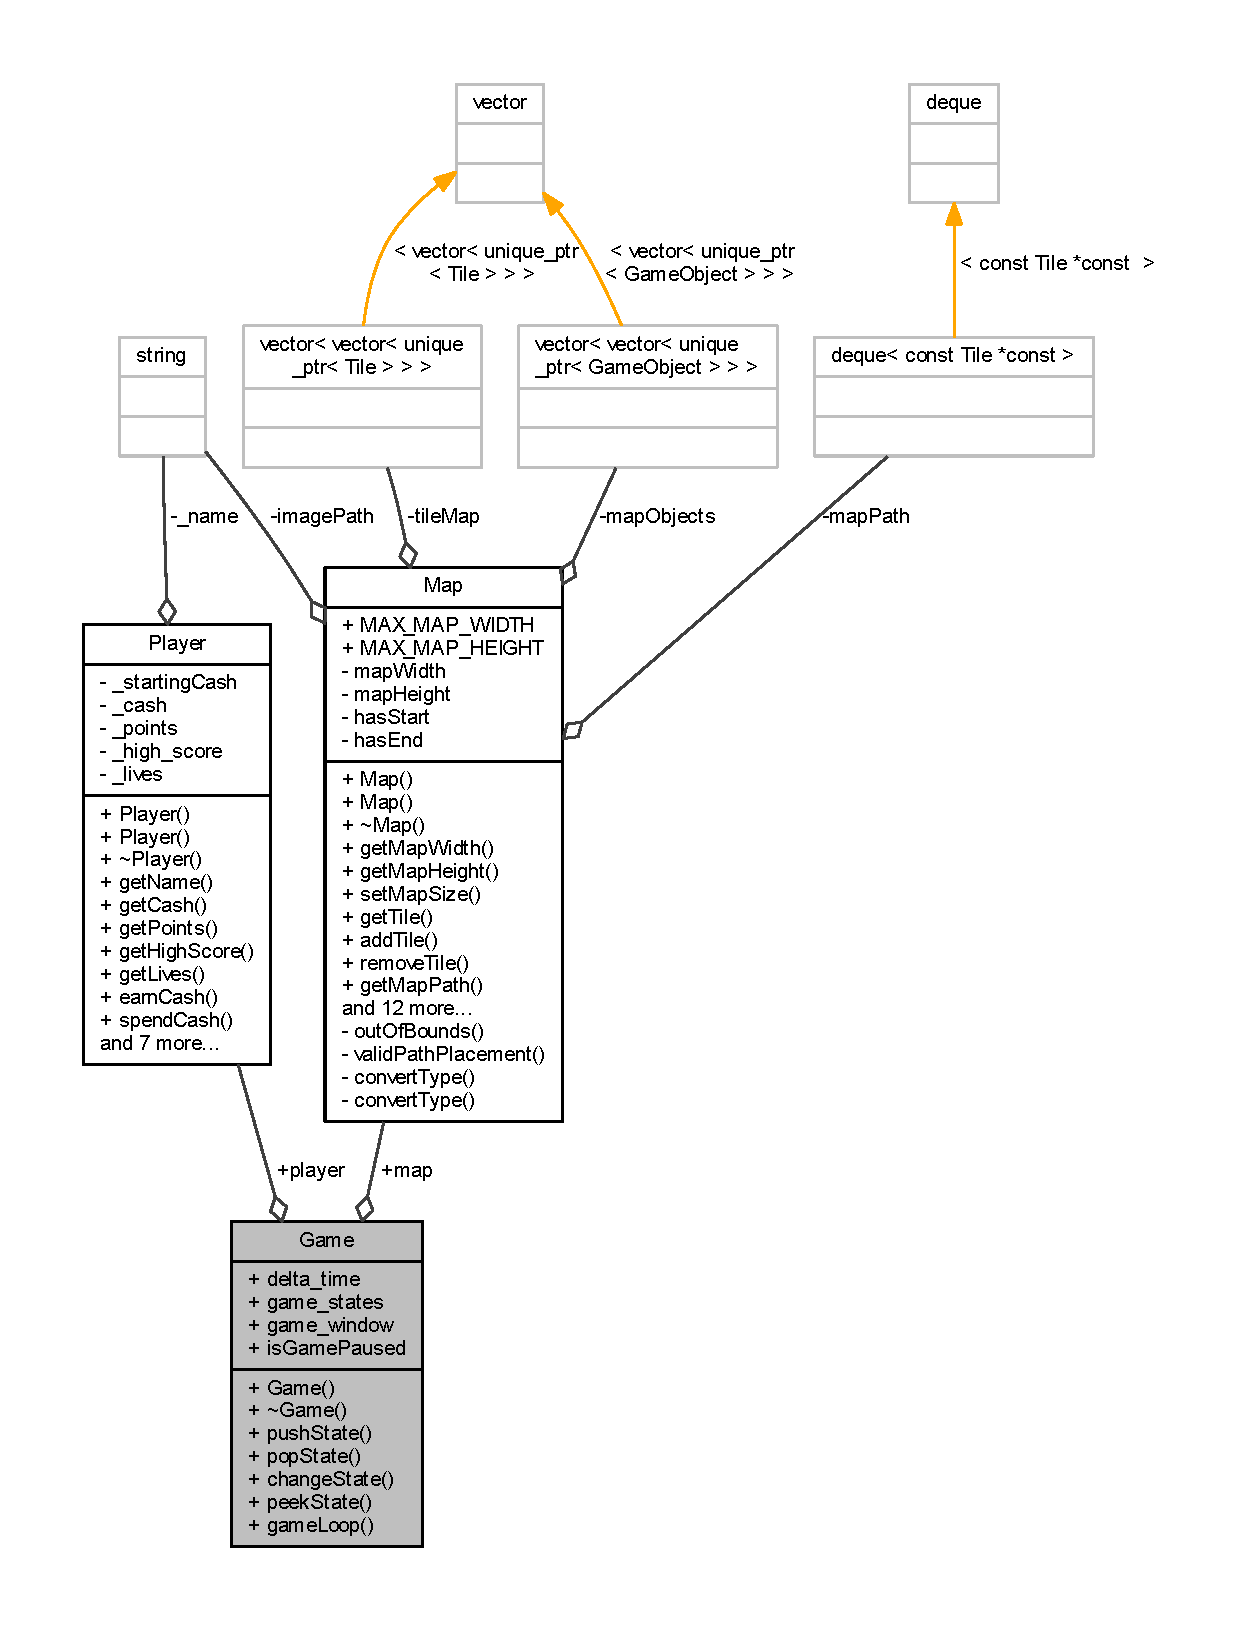
\includegraphics[width=166pt]{class_game__coll__graph}
\end{center}
\end{figure}
\subsection*{Public Member Functions}
\begin{DoxyCompactItemize}
\item 
\hyperlink{class_game_ad59df6562a58a614fda24622d3715b65}{Game} ()
\begin{DoxyCompactList}\small\item\em Constructor of \hyperlink{class_game}{Game} sets the game window properties and frame rate. \end{DoxyCompactList}\item 
\hyperlink{class_game_ae3d112ca6e0e55150d2fdbc704474530}{$\sim$\+Game} ()
\begin{DoxyCompactList}\small\item\em Destructor of \hyperlink{class_game}{Game} removes all Game\+States from game states stack. \end{DoxyCompactList}\item 
void \hyperlink{class_game_a5898f1edb6e3bc1700b2ffb1943bc609}{push\+State} (\hyperlink{class_game_state}{Game\+State} $\ast$state)
\begin{DoxyCompactList}\small\item\em Helper push function for \hyperlink{class_game_state}{Game\+State} stack. \end{DoxyCompactList}\item 
void \hyperlink{class_game_a4b33dd67adef59bebadba8a234282c88}{pop\+State} ()
\begin{DoxyCompactList}\small\item\em Helper pop function for \hyperlink{class_game_state}{Game\+State} stack. \end{DoxyCompactList}\item 
void \hyperlink{class_game_a8683b16995200bd11d95efc372e6722a}{change\+State} (\hyperlink{class_game_state}{Game\+State} $\ast$state)
\begin{DoxyCompactList}\small\item\em Helper function for \hyperlink{class_game_state}{Game\+State} stack to change previous state into given state. \end{DoxyCompactList}\item 
\hyperlink{class_game_state}{Game\+State} $\ast$ \hyperlink{class_game_a6cdc6cb374ab8e7d8ac9b280284b3793}{peek\+State} ()
\begin{DoxyCompactList}\small\item\em Helper peek function for \hyperlink{class_game_state}{Game\+State} stack. \end{DoxyCompactList}\item 
void \hyperlink{class_game_aede5f46c8c7bbbaf8459eeec397a11e7}{game\+Loop} ()
\begin{DoxyCompactList}\small\item\em Drives the game. \end{DoxyCompactList}\end{DoxyCompactItemize}
\subsection*{Public Attributes}
\begin{DoxyCompactItemize}
\item 
std\+::stack$<$ \hyperlink{class_game_state}{Game\+State} $\ast$ $>$ \hyperlink{class_game_a5ed7be8060ef5d384b62f384fb8662ed}{game\+\_\+states}
\begin{DoxyCompactList}\small\item\em Stack for storing the game states. \end{DoxyCompactList}\item 
sf\+::\+Render\+Window \hyperlink{class_game_ae19475408ec62b8ed6d4109b56d28b1d}{game\+\_\+window}
\begin{DoxyCompactList}\small\item\em Main window for game. \end{DoxyCompactList}\end{DoxyCompactItemize}


\subsection{Detailed Description}
Creates a \hyperlink{class_game}{Game}. \hyperlink{class_game}{Game} is a \hyperlink{class_game_state}{Game\+State} manager that handles the changing of the states and info storage in every game state. 

\subsection{Constructor \& Destructor Documentation}
\hypertarget{class_game_ad59df6562a58a614fda24622d3715b65}{\index{Game@{Game}!Game@{Game}}
\index{Game@{Game}!Game@{Game}}
\subsubsection[{Game}]{\setlength{\rightskip}{0pt plus 5cm}Game\+::\+Game (
\begin{DoxyParamCaption}
{}
\end{DoxyParamCaption}
)}}\label{class_game_ad59df6562a58a614fda24622d3715b65}


Constructor of \hyperlink{class_game}{Game} sets the game window properties and frame rate. 

\hypertarget{class_game_ae3d112ca6e0e55150d2fdbc704474530}{\index{Game@{Game}!````~Game@{$\sim$\+Game}}
\index{````~Game@{$\sim$\+Game}!Game@{Game}}
\subsubsection[{$\sim$\+Game}]{\setlength{\rightskip}{0pt plus 5cm}Game\+::$\sim$\+Game (
\begin{DoxyParamCaption}
{}
\end{DoxyParamCaption}
)}}\label{class_game_ae3d112ca6e0e55150d2fdbc704474530}


Destructor of \hyperlink{class_game}{Game} removes all Game\+States from game states stack. 



Here is the call graph for this function\+:
\nopagebreak
\begin{figure}[H]
\begin{center}
\leavevmode
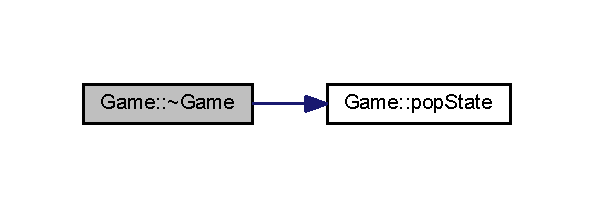
\includegraphics[width=285pt]{class_game_ae3d112ca6e0e55150d2fdbc704474530_cgraph}
\end{center}
\end{figure}




\subsection{Member Function Documentation}
\hypertarget{class_game_a8683b16995200bd11d95efc372e6722a}{\index{Game@{Game}!change\+State@{change\+State}}
\index{change\+State@{change\+State}!Game@{Game}}
\subsubsection[{change\+State}]{\setlength{\rightskip}{0pt plus 5cm}void Game\+::change\+State (
\begin{DoxyParamCaption}
\item[{{\bf Game\+State} $\ast$}]{state}
\end{DoxyParamCaption}
)}}\label{class_game_a8683b16995200bd11d95efc372e6722a}


Helper function for \hyperlink{class_game_state}{Game\+State} stack to change previous state into given state. 

\begin{DoxyReturn}{Returns}
Void. 
\end{DoxyReturn}


Here is the call graph for this function\+:
\nopagebreak
\begin{figure}[H]
\begin{center}
\leavevmode
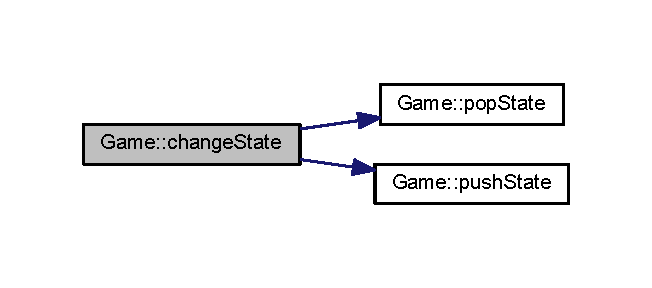
\includegraphics[width=313pt]{class_game_a8683b16995200bd11d95efc372e6722a_cgraph}
\end{center}
\end{figure}


\hypertarget{class_game_aede5f46c8c7bbbaf8459eeec397a11e7}{\index{Game@{Game}!game\+Loop@{game\+Loop}}
\index{game\+Loop@{game\+Loop}!Game@{Game}}
\subsubsection[{game\+Loop}]{\setlength{\rightskip}{0pt plus 5cm}void Game\+::game\+Loop (
\begin{DoxyParamCaption}
{}
\end{DoxyParamCaption}
)}}\label{class_game_aede5f46c8c7bbbaf8459eeec397a11e7}


Drives the game. 

\begin{DoxyReturn}{Returns}
Void.
\end{DoxyReturn}
This function controls the speed of the logic in the game and passes it to any function that needs it. since \hyperlink{class_game_aede5f46c8c7bbbaf8459eeec397a11e7}{game\+Loop()} is called every frame, this function starts the clock at the beginning of the frame, stops it at the end and calculates the elapsed time.

The functions from \hyperlink{class_game_state}{Game\+State} are then called to draw updates to the render window. Calculate elapsed time

Draw updates to render window 

Here is the call graph for this function\+:
\nopagebreak
\begin{figure}[H]
\begin{center}
\leavevmode
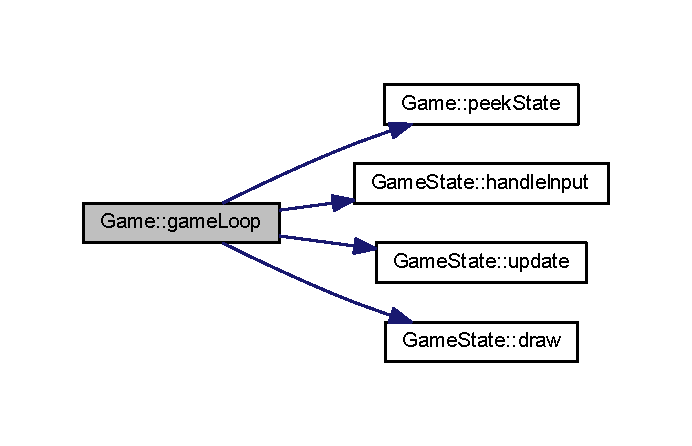
\includegraphics[width=332pt]{class_game_aede5f46c8c7bbbaf8459eeec397a11e7_cgraph}
\end{center}
\end{figure}




Here is the caller graph for this function\+:
\nopagebreak
\begin{figure}[H]
\begin{center}
\leavevmode
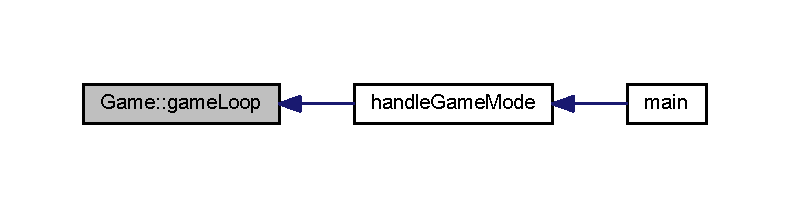
\includegraphics[width=248pt]{class_game_aede5f46c8c7bbbaf8459eeec397a11e7_icgraph}
\end{center}
\end{figure}


\hypertarget{class_game_a6cdc6cb374ab8e7d8ac9b280284b3793}{\index{Game@{Game}!peek\+State@{peek\+State}}
\index{peek\+State@{peek\+State}!Game@{Game}}
\subsubsection[{peek\+State}]{\setlength{\rightskip}{0pt plus 5cm}{\bf Game\+State} $\ast$ Game\+::peek\+State (
\begin{DoxyParamCaption}
{}
\end{DoxyParamCaption}
)}}\label{class_game_a6cdc6cb374ab8e7d8ac9b280284b3793}


Helper peek function for \hyperlink{class_game_state}{Game\+State} stack. 

\begin{DoxyReturn}{Returns}
Pointer to \hyperlink{class_game_state}{Game\+State} that's on top of the stack. 
\end{DoxyReturn}


Here is the caller graph for this function\+:
\nopagebreak
\begin{figure}[H]
\begin{center}
\leavevmode
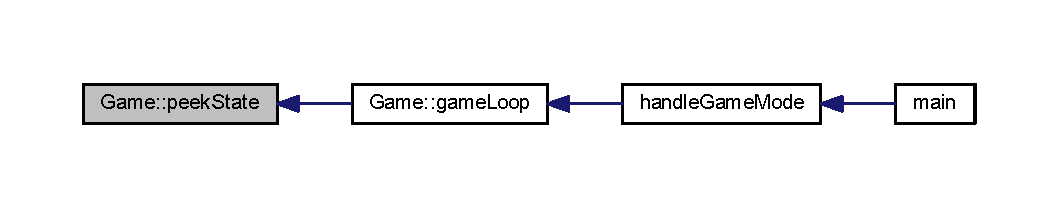
\includegraphics[width=350pt]{class_game_a6cdc6cb374ab8e7d8ac9b280284b3793_icgraph}
\end{center}
\end{figure}


\hypertarget{class_game_a4b33dd67adef59bebadba8a234282c88}{\index{Game@{Game}!pop\+State@{pop\+State}}
\index{pop\+State@{pop\+State}!Game@{Game}}
\subsubsection[{pop\+State}]{\setlength{\rightskip}{0pt plus 5cm}void Game\+::pop\+State (
\begin{DoxyParamCaption}
{}
\end{DoxyParamCaption}
)}}\label{class_game_a4b33dd67adef59bebadba8a234282c88}


Helper pop function for \hyperlink{class_game_state}{Game\+State} stack. 

\begin{DoxyReturn}{Returns}
Void. 
\end{DoxyReturn}


Here is the caller graph for this function\+:
\nopagebreak
\begin{figure}[H]
\begin{center}
\leavevmode
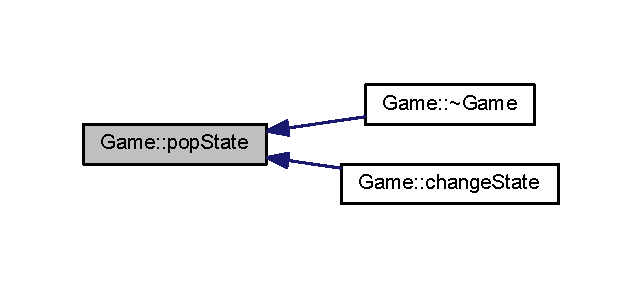
\includegraphics[width=308pt]{class_game_a4b33dd67adef59bebadba8a234282c88_icgraph}
\end{center}
\end{figure}


\hypertarget{class_game_a5898f1edb6e3bc1700b2ffb1943bc609}{\index{Game@{Game}!push\+State@{push\+State}}
\index{push\+State@{push\+State}!Game@{Game}}
\subsubsection[{push\+State}]{\setlength{\rightskip}{0pt plus 5cm}void Game\+::push\+State (
\begin{DoxyParamCaption}
\item[{{\bf Game\+State} $\ast$}]{state}
\end{DoxyParamCaption}
)}}\label{class_game_a5898f1edb6e3bc1700b2ffb1943bc609}


Helper push function for \hyperlink{class_game_state}{Game\+State} stack. 

\begin{DoxyReturn}{Returns}
Void. 
\end{DoxyReturn}


Here is the caller graph for this function\+:
\nopagebreak
\begin{figure}[H]
\begin{center}
\leavevmode
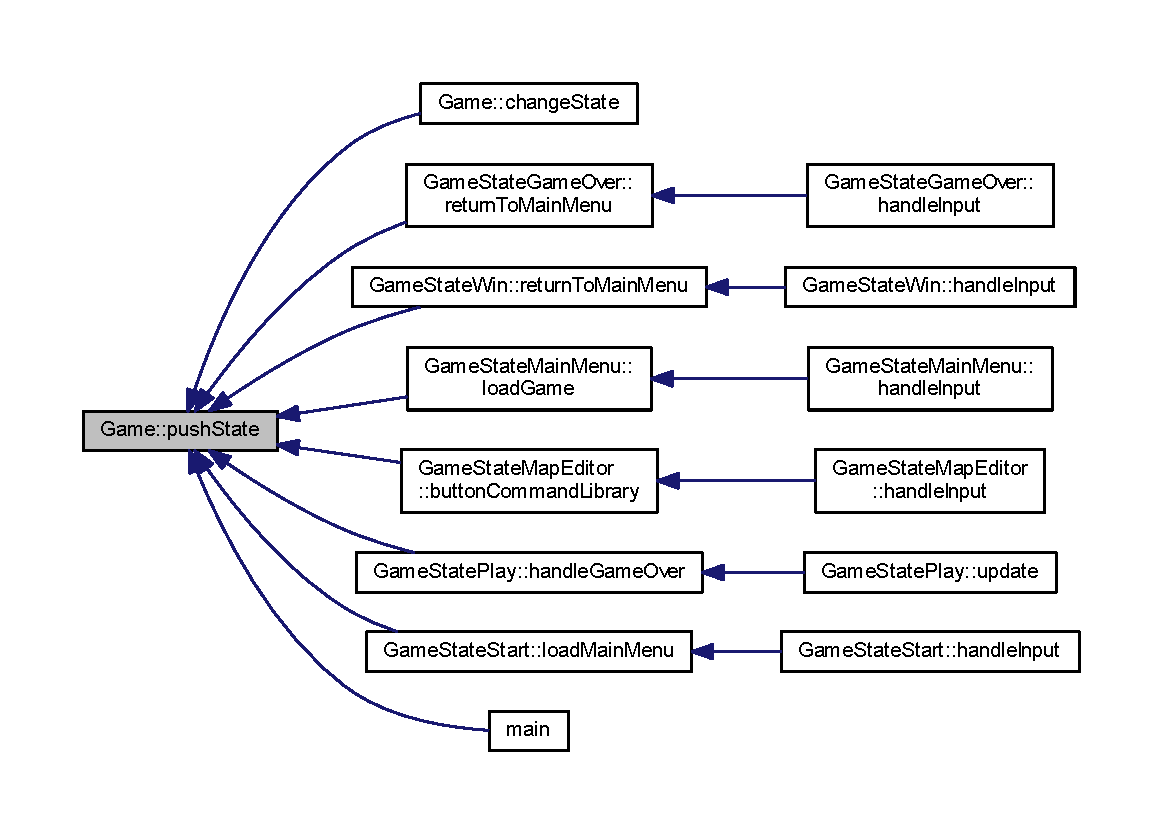
\includegraphics[width=350pt]{class_game_a5898f1edb6e3bc1700b2ffb1943bc609_icgraph}
\end{center}
\end{figure}




\subsection{Member Data Documentation}
\hypertarget{class_game_a5ed7be8060ef5d384b62f384fb8662ed}{\index{Game@{Game}!game\+\_\+states@{game\+\_\+states}}
\index{game\+\_\+states@{game\+\_\+states}!Game@{Game}}
\subsubsection[{game\+\_\+states}]{\setlength{\rightskip}{0pt plus 5cm}std\+::stack$<${\bf Game\+State}$\ast$$>$ Game\+::game\+\_\+states}}\label{class_game_a5ed7be8060ef5d384b62f384fb8662ed}


Stack for storing the game states. 

\hypertarget{class_game_ae19475408ec62b8ed6d4109b56d28b1d}{\index{Game@{Game}!game\+\_\+window@{game\+\_\+window}}
\index{game\+\_\+window@{game\+\_\+window}!Game@{Game}}
\subsubsection[{game\+\_\+window}]{\setlength{\rightskip}{0pt plus 5cm}sf\+::\+Render\+Window Game\+::game\+\_\+window}}\label{class_game_ae19475408ec62b8ed6d4109b56d28b1d}


Main window for game. 



The documentation for this class was generated from the following files\+:\begin{DoxyCompactItemize}
\item 
jamms/\+Tower\+Defense/\+Tower\+Defense/include/\hyperlink{_game_8h}{Game.\+h}\item 
jamms/\+Tower\+Defense/\+Tower\+Defense/src/\hyperlink{_game_8cpp}{Game.\+cpp}\end{DoxyCompactItemize}

\hypertarget{class_game_object}{\section{Game\+Object Class Reference}
\label{class_game_object}\index{Game\+Object@{Game\+Object}}
}


Creates a \hyperlink{class_game_object}{Game\+Object}. \hyperlink{class_game_object}{Game\+Object} is a class that creates all objects seen in the application. Each \hyperlink{class_game_object}{Game\+Object} instance creates a sprite at a specified position. Game\+Objects can then be drawn to the render window.  




{\ttfamily \#include $<$Game\+Object.\+h$>$}



Inheritance diagram for Game\+Object\+:
\nopagebreak
\begin{figure}[H]
\begin{center}
\leavevmode
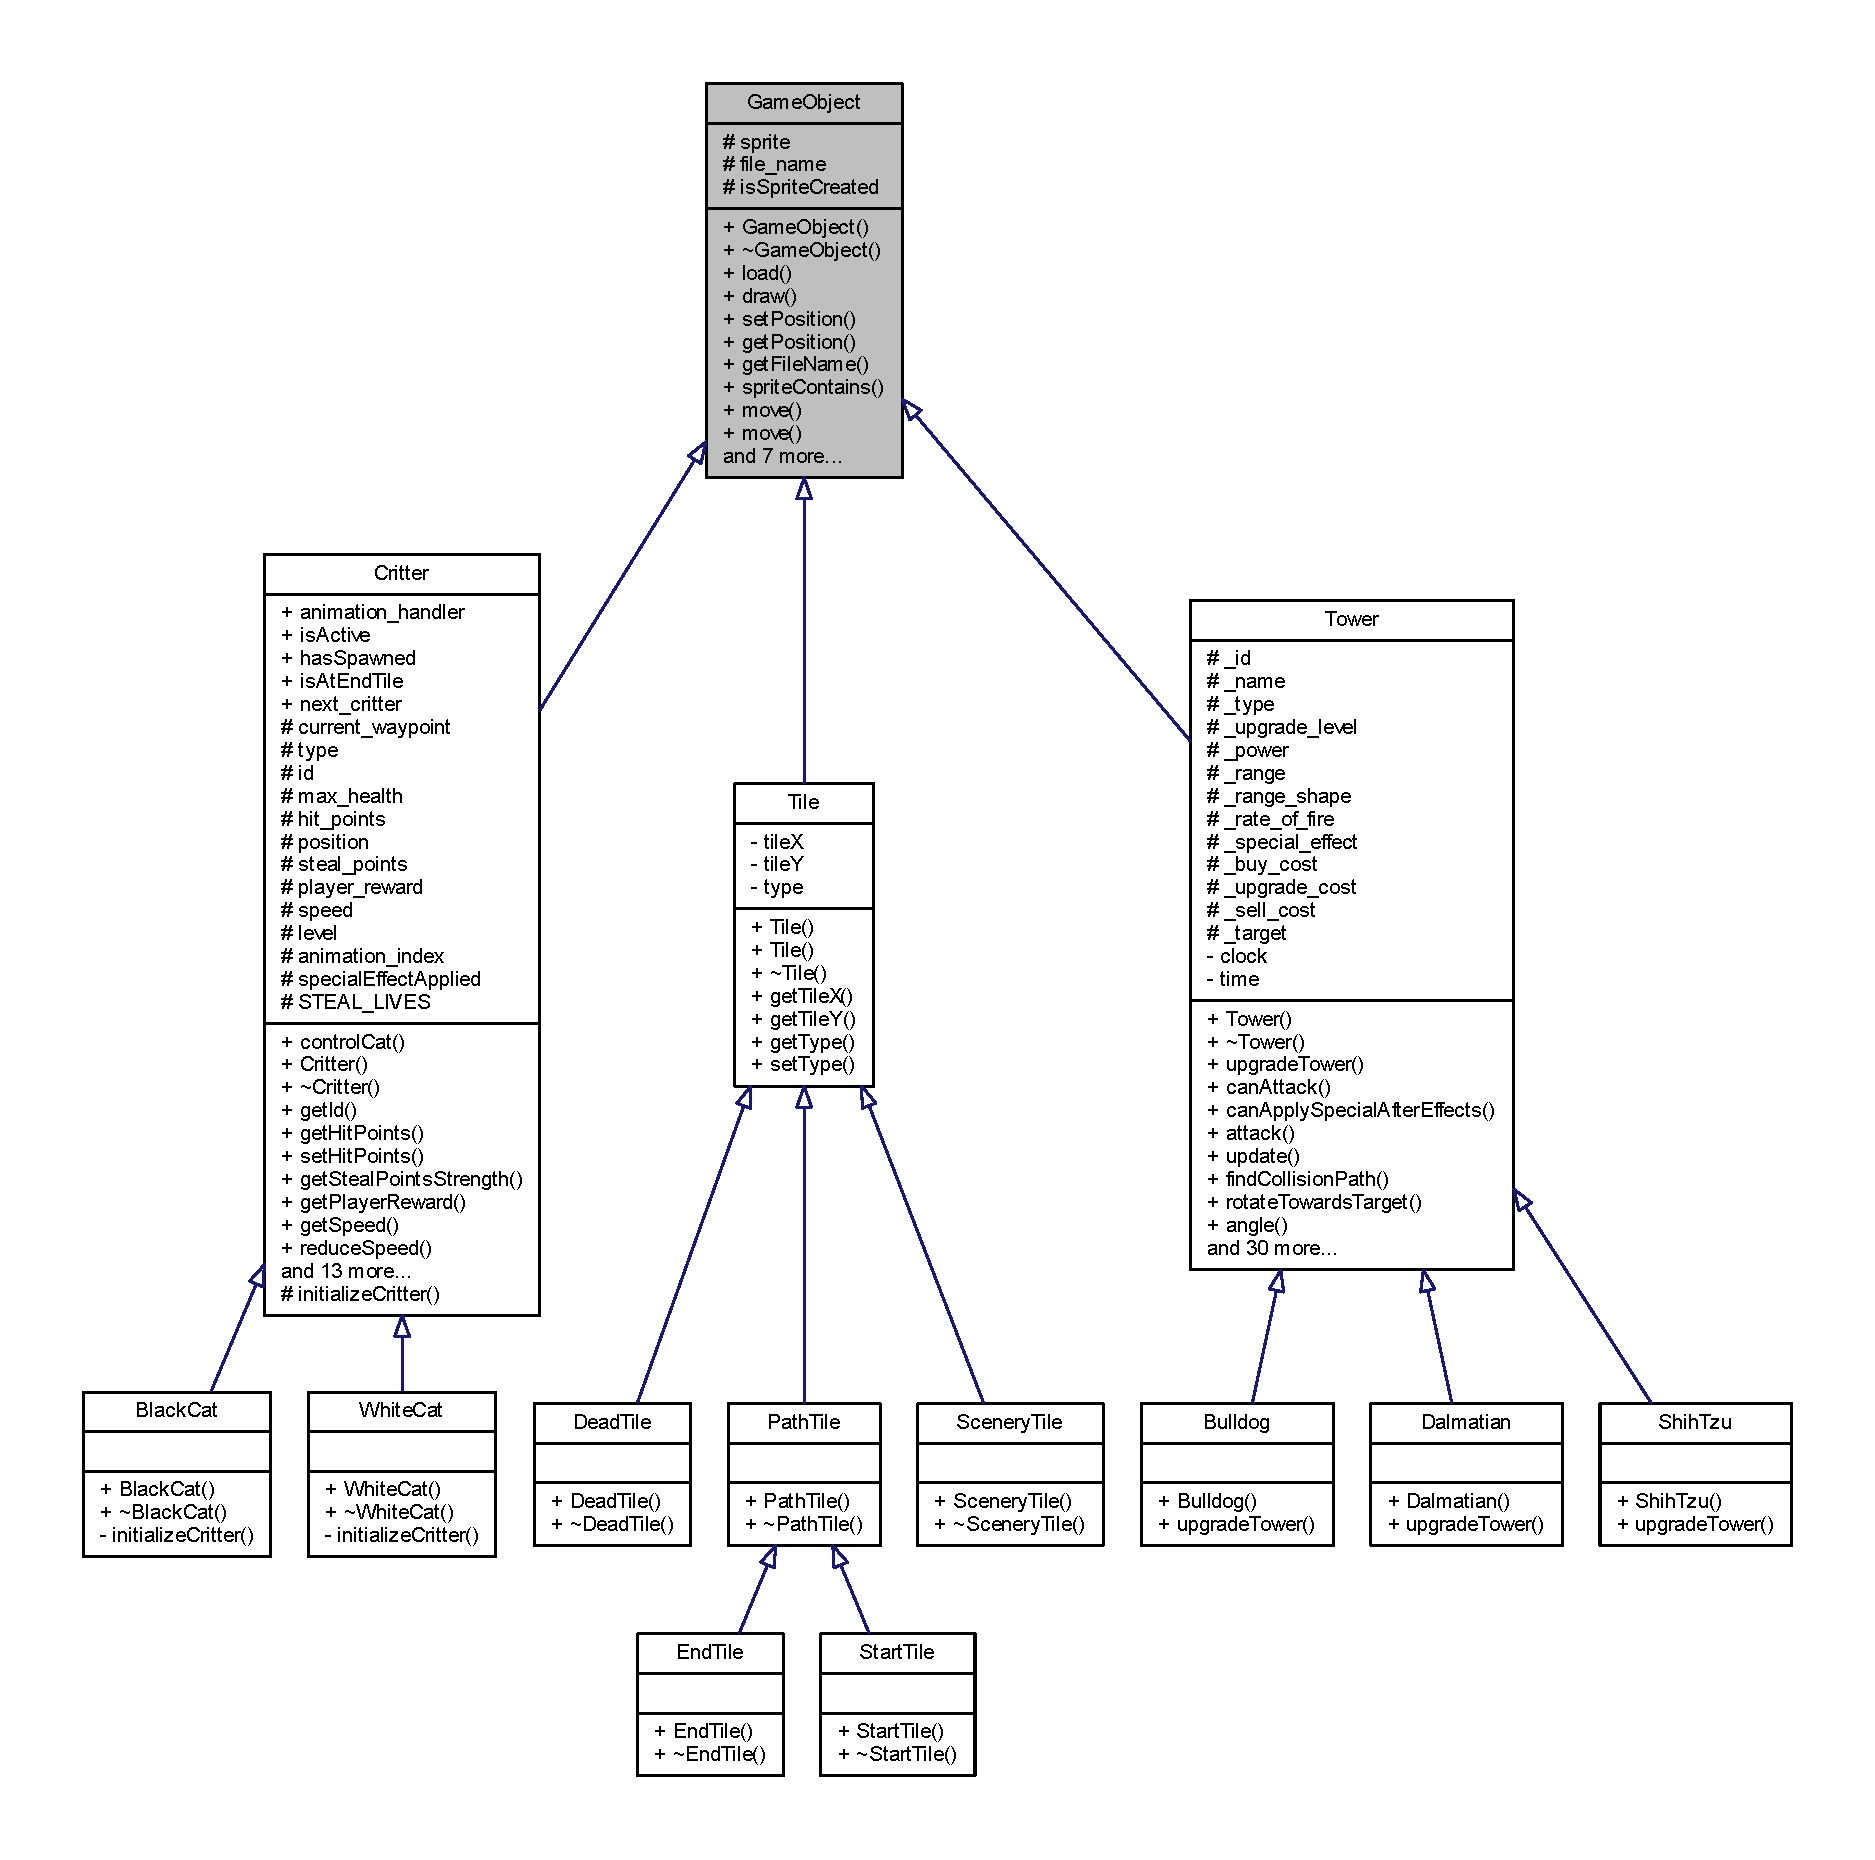
\includegraphics[width=350pt]{class_game_object__inherit__graph}
\end{center}
\end{figure}


Collaboration diagram for Game\+Object\+:
\nopagebreak
\begin{figure}[H]
\begin{center}
\leavevmode
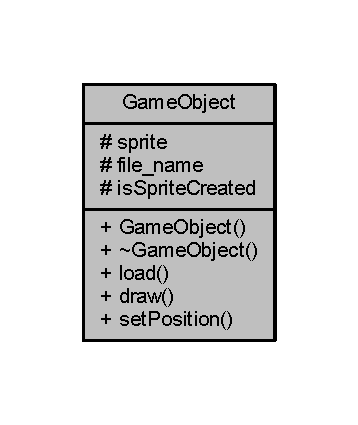
\includegraphics[width=177pt]{class_game_object__coll__graph}
\end{center}
\end{figure}
\subsection*{Public Member Functions}
\begin{DoxyCompactItemize}
\item 
\hyperlink{class_game_object_a0348e3ee2e83d56eafca7a3547f432c4}{Game\+Object} ()
\begin{DoxyCompactList}\small\item\em The \hyperlink{class_game_object}{Game\+Object} constructor. Default setup is the sprite has not been created. \end{DoxyCompactList}\item 
virtual \hyperlink{class_game_object_a224d4f6d9dd75c8a6f9d022eaf586fd9}{$\sim$\+Game\+Object} ()
\item 
virtual void \hyperlink{class_game_object_acc593e5b75a58c4a59ad59da654ce807}{load} (std\+::string \hyperlink{class_game_object_a1b725daa9c79833a7139469468dc770a}{file\+\_\+name})
\begin{DoxyCompactList}\small\item\em Loads a texture using the \hyperlink{class_texture_manager}{Texture\+Manager} class and creates a sprite. \end{DoxyCompactList}\item 
virtual void \hyperlink{class_game_object_abf4de46e52c8f23d18d51bc29744b136}{draw} (sf\+::\+Render\+Window \&window)
\begin{DoxyCompactList}\small\item\em Draws a sprite to the render window if the \hyperlink{class_game_object}{Game\+Object} instance has previously been loaded. \end{DoxyCompactList}\item 
virtual void \hyperlink{class_game_object_a180d6e9e7afa44b30ca678a95c6f4dad}{set\+Position} (float x, float y)
\begin{DoxyCompactList}\small\item\em Sets the initial draw position of a \hyperlink{class_game_object}{Game\+Object} instance. \end{DoxyCompactList}\item 
virtual std\+::pair$<$ float, float $>$ \hyperlink{class_game_object_ad568496dd9cee5b9edd9357d30a00dff}{get\+Position} () const 
\begin{DoxyCompactList}\small\item\em Converts and retrieves an pair$<$float, float$>$ object from a sf\+::vector2f. \end{DoxyCompactList}\item 
std\+::string \hyperlink{class_game_object_a387e235ced0f778e58d5f4a39f58a220}{get\+File\+Name} () const 
\item 
bool \hyperlink{class_game_object_adf7e04407f7c2a5bd487b459efe9fd79}{sprite\+Contains} (sf\+::\+Vector2i \hyperlink{class_game_object_a86e4253e3734436b4a5a0c503e0033b4}{position}) const 
\item 
virtual void \hyperlink{class_game_object_a6fa0d948eccbd0345cda6bdea5b5196a}{move} (float x, float y)
\item 
virtual void \hyperlink{class_game_object_a3ad77a6b8bc1adfb8ea463f12c022b1e}{move} (const sf\+::\+Vector2f \&offset)
\item 
virtual sf\+::\+Float\+Rect \hyperlink{class_game_object_a3a1df73c1ffc15d9bb616aebc3e477fd}{get\+Global\+Bounds} () const 
\begin{DoxyCompactList}\small\item\em Retrieves the floating recantle encompassing a sprite (after the result of transormations) \end{DoxyCompactList}\item 
virtual bool \hyperlink{class_game_object_a18a09c750e617f7e3188bda15a7d5fd7}{box\+To\+Box\+Intersection} (\hyperlink{class_game_object}{Game\+Object} $\ast$game\+\_\+object)
\begin{DoxyCompactList}\small\item\em Bouding box intersection between Game\+Objects. \end{DoxyCompactList}\item 
virtual bool \hyperlink{class_game_object_a3a9fd4ee6157fcf61fd8f7d7318598c5}{circle\+To\+Circle\+Intersection} (\hyperlink{class_game_object}{Game\+Object} $\ast$game\+\_\+object)
\begin{DoxyCompactList}\small\item\em Measures the distance between the centers of each object to each other and compare that with their radii. \end{DoxyCompactList}\item 
virtual std\+::pair$<$ float, float $>$ \hyperlink{class_game_object_ad6d60e0c273cb0074c91a19f3aed8708}{get\+Sprite\+Center} ()
\begin{DoxyCompactList}\small\item\em Gets the center of a sprite. \end{DoxyCompactList}\item 
virtual std\+::pair$<$ float, float $>$ \hyperlink{class_game_object_a3731c03ddcbdb904bd41af78e09d262a}{get\+Sprite\+Size} ()
\begin{DoxyCompactList}\small\item\em Gets the size of a sprite. \end{DoxyCompactList}\item 
virtual float \hyperlink{class_game_object_a8220201988f2aaea8a6f748872e188a9}{get\+Rectangle\+Sprite\+Radius} ()
\begin{DoxyCompactList}\small\item\em Measures the radius of the rectangle sprite. \end{DoxyCompactList}\item 
virtual void \hyperlink{class_game_object_a320a94559557834d53bffa538d8349c9}{set\+Rotation} (float angle)
\end{DoxyCompactItemize}
\subsection*{Protected Attributes}
\begin{DoxyCompactItemize}
\item 
sf\+::\+Vector2f \hyperlink{class_game_object_a86e4253e3734436b4a5a0c503e0033b4}{position}
\item 
sf\+::\+Sprite \hyperlink{class_game_object_abb3608f1c76edd590e023585c2216f02}{sprite}
\begin{DoxyCompactList}\small\item\em The Sprite instance of the \hyperlink{class_game_object}{Game\+Object}. \end{DoxyCompactList}\item 
std\+::string \hyperlink{class_game_object_a1b725daa9c79833a7139469468dc770a}{file\+\_\+name}
\begin{DoxyCompactList}\small\item\em The file name of the sprite's texture. \end{DoxyCompactList}\item 
bool \hyperlink{class_game_object_a677286bcb906871b6a3eb0c0b9342176}{is\+Sprite\+Created}
\begin{DoxyCompactList}\small\item\em Boolean indicating whether or not a sprite has been created. The purpose of this bool is to ensure that the sprite exists before the class attempts to draw the \hyperlink{class_game_object}{Game\+Object}. \end{DoxyCompactList}\end{DoxyCompactItemize}


\subsection{Detailed Description}
Creates a \hyperlink{class_game_object}{Game\+Object}. \hyperlink{class_game_object}{Game\+Object} is a class that creates all objects seen in the application. Each \hyperlink{class_game_object}{Game\+Object} instance creates a sprite at a specified position. Game\+Objects can then be drawn to the render window. 

\subsection{Constructor \& Destructor Documentation}
\hypertarget{class_game_object_a0348e3ee2e83d56eafca7a3547f432c4}{\index{Game\+Object@{Game\+Object}!Game\+Object@{Game\+Object}}
\index{Game\+Object@{Game\+Object}!Game\+Object@{Game\+Object}}
\subsubsection[{Game\+Object}]{\setlength{\rightskip}{0pt plus 5cm}Game\+Object\+::\+Game\+Object (
\begin{DoxyParamCaption}
{}
\end{DoxyParamCaption}
)}}\label{class_game_object_a0348e3ee2e83d56eafca7a3547f432c4}


The \hyperlink{class_game_object}{Game\+Object} constructor. Default setup is the sprite has not been created. 

\hypertarget{class_game_object_a224d4f6d9dd75c8a6f9d022eaf586fd9}{\index{Game\+Object@{Game\+Object}!````~Game\+Object@{$\sim$\+Game\+Object}}
\index{````~Game\+Object@{$\sim$\+Game\+Object}!Game\+Object@{Game\+Object}}
\subsubsection[{$\sim$\+Game\+Object}]{\setlength{\rightskip}{0pt plus 5cm}virtual Game\+Object\+::$\sim$\+Game\+Object (
\begin{DoxyParamCaption}
{}
\end{DoxyParamCaption}
)\hspace{0.3cm}{\ttfamily [inline]}, {\ttfamily [virtual]}}}\label{class_game_object_a224d4f6d9dd75c8a6f9d022eaf586fd9}


\subsection{Member Function Documentation}
\hypertarget{class_game_object_a18a09c750e617f7e3188bda15a7d5fd7}{\index{Game\+Object@{Game\+Object}!box\+To\+Box\+Intersection@{box\+To\+Box\+Intersection}}
\index{box\+To\+Box\+Intersection@{box\+To\+Box\+Intersection}!Game\+Object@{Game\+Object}}
\subsubsection[{box\+To\+Box\+Intersection}]{\setlength{\rightskip}{0pt plus 5cm}bool Game\+Object\+::box\+To\+Box\+Intersection (
\begin{DoxyParamCaption}
\item[{{\bf Game\+Object} $\ast$}]{game\+\_\+object}
\end{DoxyParamCaption}
)\hspace{0.3cm}{\ttfamily [virtual]}}}\label{class_game_object_a18a09c750e617f7e3188bda15a7d5fd7}


Bouding box intersection between Game\+Objects. 

\begin{DoxyReturn}{Returns}
bool 
\end{DoxyReturn}


Here is the call graph for this function\+:\nopagebreak
\begin{figure}[H]
\begin{center}
\leavevmode
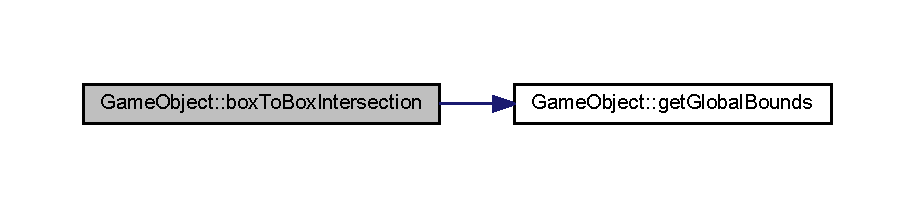
\includegraphics[width=350pt]{class_game_object_a18a09c750e617f7e3188bda15a7d5fd7_cgraph}
\end{center}
\end{figure}


\hypertarget{class_game_object_a3a9fd4ee6157fcf61fd8f7d7318598c5}{\index{Game\+Object@{Game\+Object}!circle\+To\+Circle\+Intersection@{circle\+To\+Circle\+Intersection}}
\index{circle\+To\+Circle\+Intersection@{circle\+To\+Circle\+Intersection}!Game\+Object@{Game\+Object}}
\subsubsection[{circle\+To\+Circle\+Intersection}]{\setlength{\rightskip}{0pt plus 5cm}bool Game\+Object\+::circle\+To\+Circle\+Intersection (
\begin{DoxyParamCaption}
\item[{{\bf Game\+Object} $\ast$}]{game\+\_\+object}
\end{DoxyParamCaption}
)\hspace{0.3cm}{\ttfamily [virtual]}}}\label{class_game_object_a3a9fd4ee6157fcf61fd8f7d7318598c5}


Measures the distance between the centers of each object to each other and compare that with their radii. 

\begin{DoxyReturn}{Returns}
bool 
\end{DoxyReturn}


Reimplemented in \hyperlink{class_tower_a518ff249dec05cdd026a830d845abfd2}{Tower}, and \hyperlink{class_tower_game_object_a824c0212a0c2958d9facfa97947c7332}{Tower\+Game\+Object}.



Here is the call graph for this function\+:
\nopagebreak
\begin{figure}[H]
\begin{center}
\leavevmode
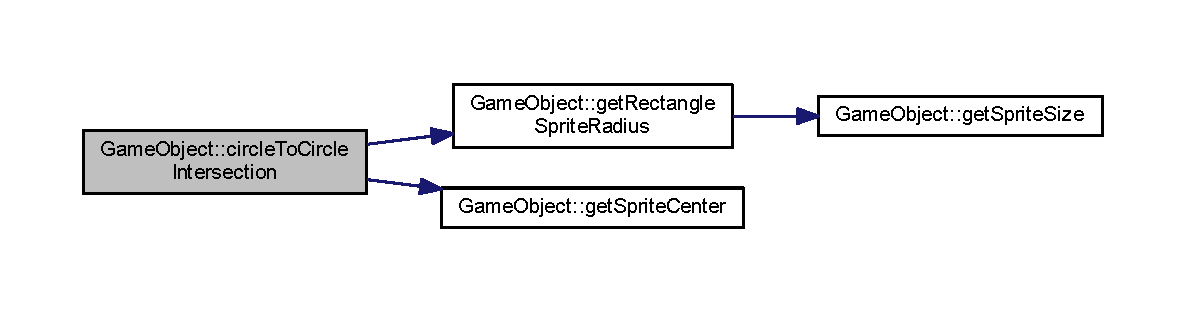
\includegraphics[width=350pt]{class_game_object_a3a9fd4ee6157fcf61fd8f7d7318598c5_cgraph}
\end{center}
\end{figure}


\hypertarget{class_game_object_abf4de46e52c8f23d18d51bc29744b136}{\index{Game\+Object@{Game\+Object}!draw@{draw}}
\index{draw@{draw}!Game\+Object@{Game\+Object}}
\subsubsection[{draw}]{\setlength{\rightskip}{0pt plus 5cm}void Game\+Object\+::draw (
\begin{DoxyParamCaption}
\item[{sf\+::\+Render\+Window \&}]{render\+\_\+window}
\end{DoxyParamCaption}
)\hspace{0.3cm}{\ttfamily [virtual]}}}\label{class_game_object_abf4de46e52c8f23d18d51bc29744b136}


Draws a sprite to the render window if the \hyperlink{class_game_object}{Game\+Object} instance has previously been loaded. 


\begin{DoxyParams}{Parameters}
{\em window} & A reference to the main render window of the application. \\
\hline
\end{DoxyParams}
\begin{DoxyReturn}{Returns}
Void.
\end{DoxyReturn}
\hyperlink{class_game_object_abf4de46e52c8f23d18d51bc29744b136}{draw()} takes in a reference to a rendering window and checks if sprite is created, if it has been, the sprite is drawn to the window. 

Here is the caller graph for this function\+:\nopagebreak
\begin{figure}[H]
\begin{center}
\leavevmode
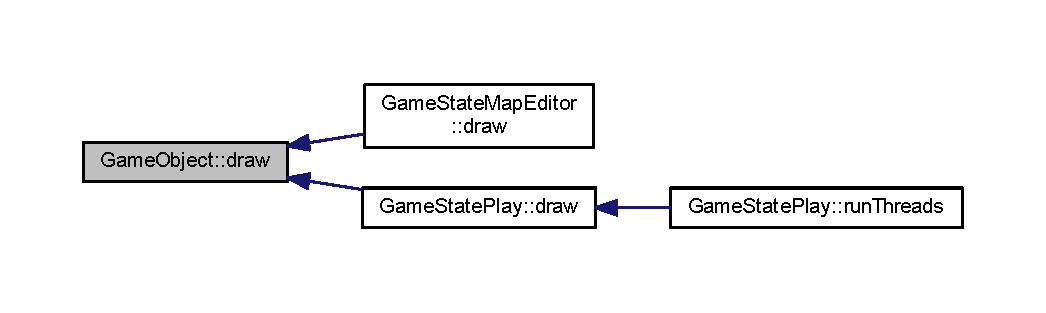
\includegraphics[width=350pt]{class_game_object_abf4de46e52c8f23d18d51bc29744b136_icgraph}
\end{center}
\end{figure}


\hypertarget{class_game_object_a387e235ced0f778e58d5f4a39f58a220}{\index{Game\+Object@{Game\+Object}!get\+File\+Name@{get\+File\+Name}}
\index{get\+File\+Name@{get\+File\+Name}!Game\+Object@{Game\+Object}}
\subsubsection[{get\+File\+Name}]{\setlength{\rightskip}{0pt plus 5cm}std\+::string Game\+Object\+::get\+File\+Name (
\begin{DoxyParamCaption}
{}
\end{DoxyParamCaption}
) const}}\label{class_game_object_a387e235ced0f778e58d5f4a39f58a220}
\hypertarget{class_game_object_a3a1df73c1ffc15d9bb616aebc3e477fd}{\index{Game\+Object@{Game\+Object}!get\+Global\+Bounds@{get\+Global\+Bounds}}
\index{get\+Global\+Bounds@{get\+Global\+Bounds}!Game\+Object@{Game\+Object}}
\subsubsection[{get\+Global\+Bounds}]{\setlength{\rightskip}{0pt plus 5cm}sf\+::\+Float\+Rect Game\+Object\+::get\+Global\+Bounds (
\begin{DoxyParamCaption}
{}
\end{DoxyParamCaption}
) const\hspace{0.3cm}{\ttfamily [virtual]}}}\label{class_game_object_a3a1df73c1ffc15d9bb616aebc3e477fd}


Retrieves the floating recantle encompassing a sprite (after the result of transormations) 

\begin{DoxyReturn}{Returns}
sf\+::\+Float\+Rect 
\end{DoxyReturn}


Here is the caller graph for this function\+:\nopagebreak
\begin{figure}[H]
\begin{center}
\leavevmode
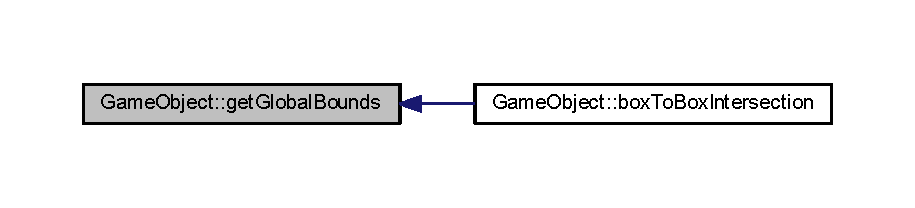
\includegraphics[width=350pt]{class_game_object_a3a1df73c1ffc15d9bb616aebc3e477fd_icgraph}
\end{center}
\end{figure}


\hypertarget{class_game_object_ad568496dd9cee5b9edd9357d30a00dff}{\index{Game\+Object@{Game\+Object}!get\+Position@{get\+Position}}
\index{get\+Position@{get\+Position}!Game\+Object@{Game\+Object}}
\subsubsection[{get\+Position}]{\setlength{\rightskip}{0pt plus 5cm}std\+::pair$<$ float, float $>$ Game\+Object\+::get\+Position (
\begin{DoxyParamCaption}
{}
\end{DoxyParamCaption}
) const\hspace{0.3cm}{\ttfamily [virtual]}}}\label{class_game_object_ad568496dd9cee5b9edd9357d30a00dff}


Converts and retrieves an pair$<$float, float$>$ object from a sf\+::vector2f. 

\begin{DoxyReturn}{Returns}
std\+::pair$<$float, float$>$ 
\end{DoxyReturn}


Here is the caller graph for this function\+:
\nopagebreak
\begin{figure}[H]
\begin{center}
\leavevmode
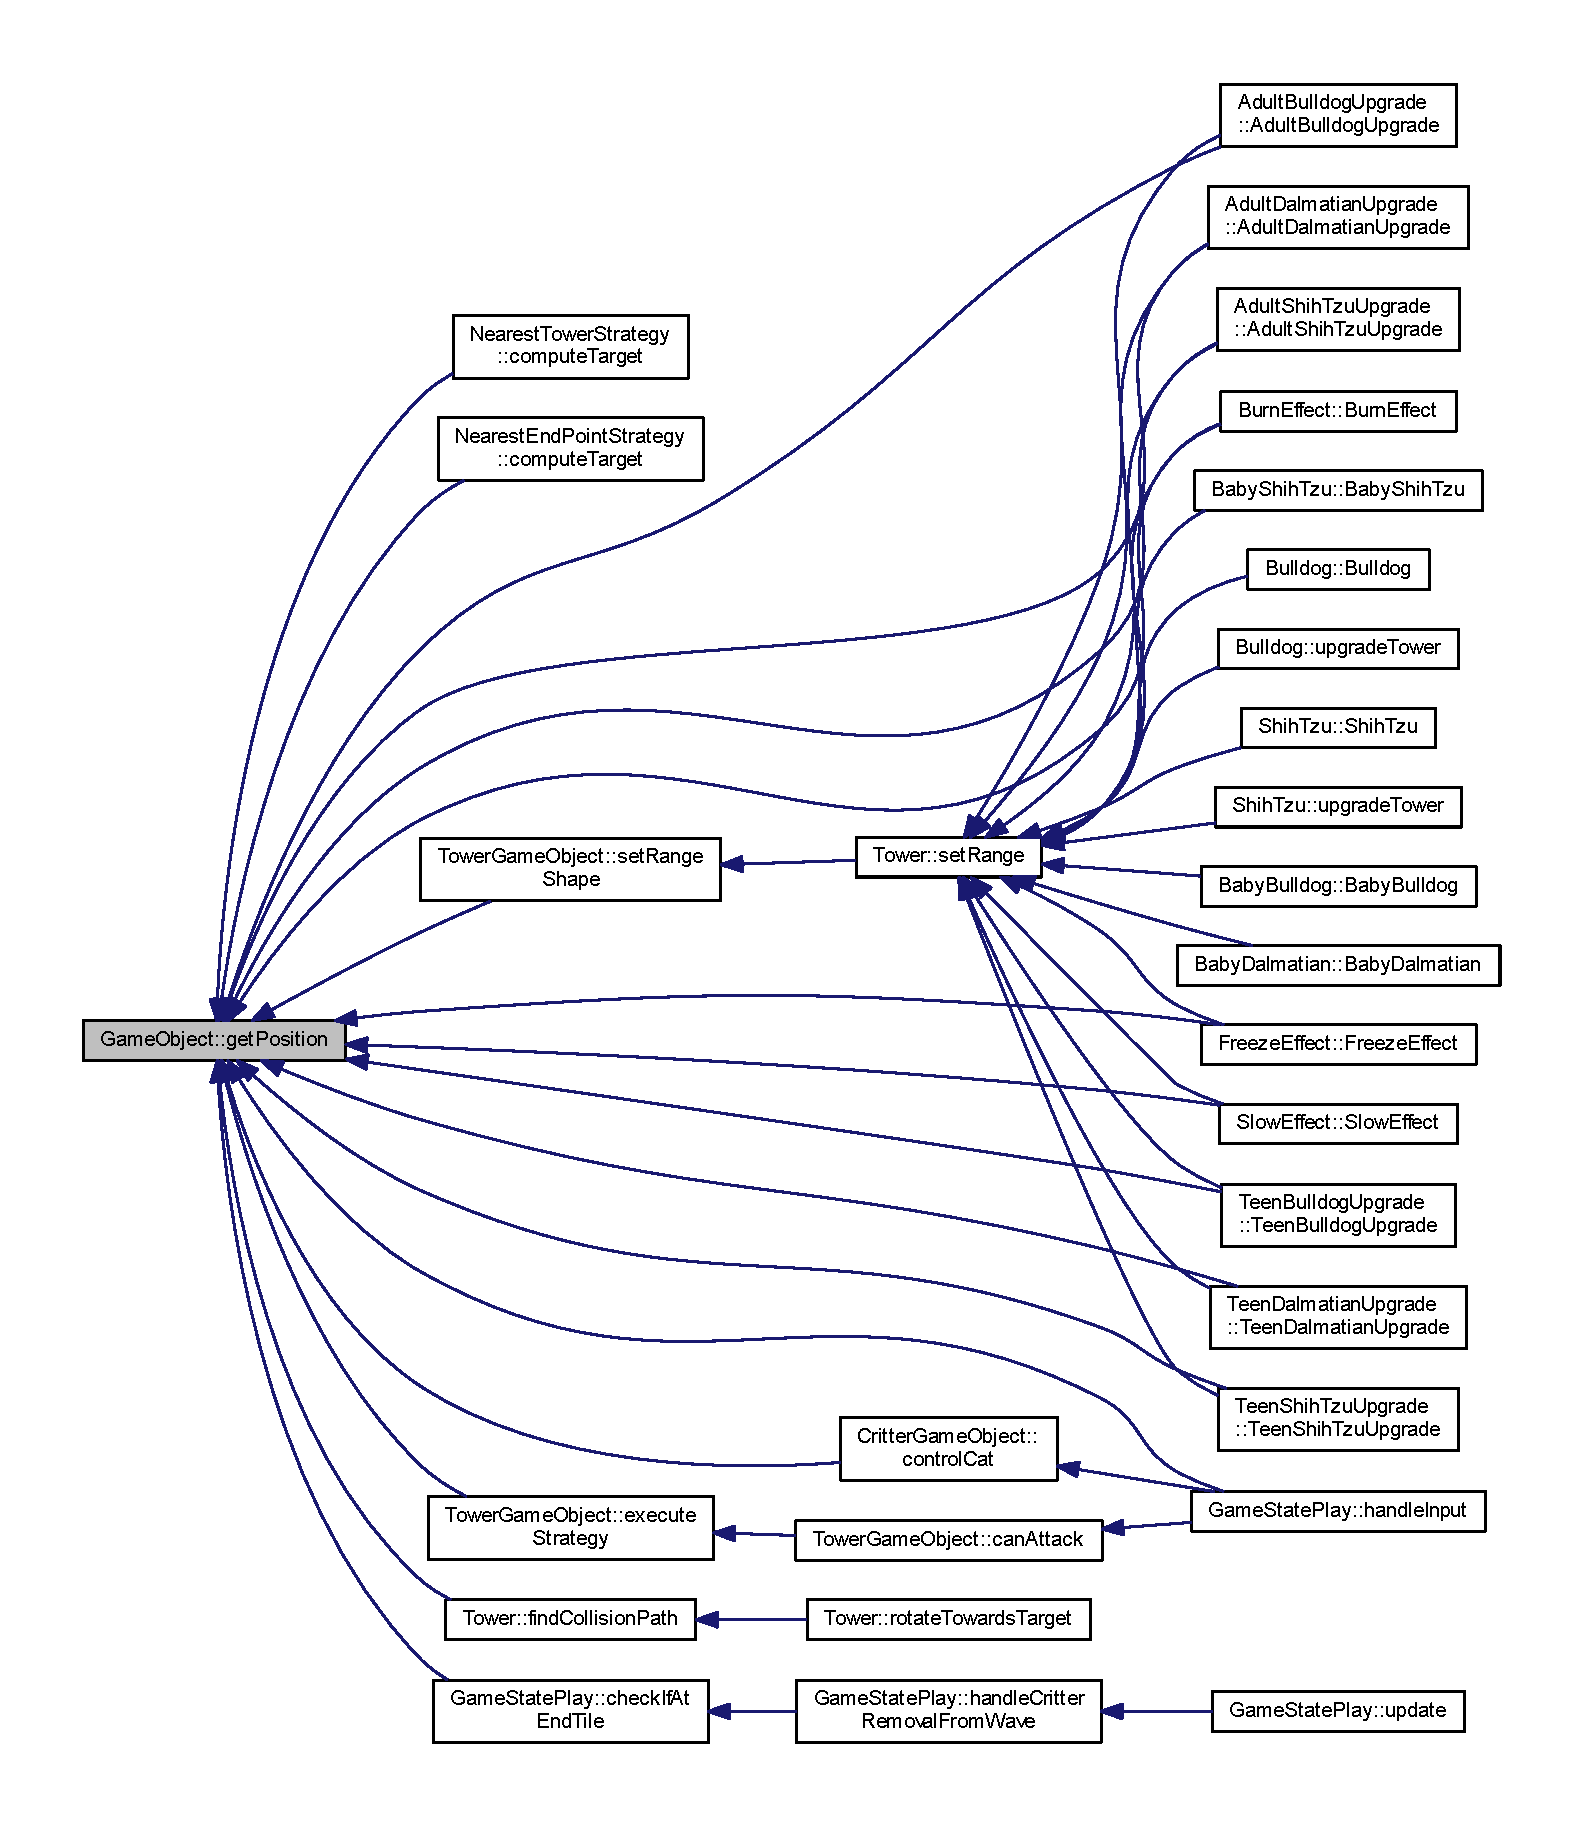
\includegraphics[width=350pt]{class_game_object_ad568496dd9cee5b9edd9357d30a00dff_icgraph}
\end{center}
\end{figure}


\hypertarget{class_game_object_a8220201988f2aaea8a6f748872e188a9}{\index{Game\+Object@{Game\+Object}!get\+Rectangle\+Sprite\+Radius@{get\+Rectangle\+Sprite\+Radius}}
\index{get\+Rectangle\+Sprite\+Radius@{get\+Rectangle\+Sprite\+Radius}!Game\+Object@{Game\+Object}}
\subsubsection[{get\+Rectangle\+Sprite\+Radius}]{\setlength{\rightskip}{0pt plus 5cm}float Game\+Object\+::get\+Rectangle\+Sprite\+Radius (
\begin{DoxyParamCaption}
{}
\end{DoxyParamCaption}
)\hspace{0.3cm}{\ttfamily [virtual]}}}\label{class_game_object_a8220201988f2aaea8a6f748872e188a9}


Measures the radius of the rectangle sprite. 

\begin{DoxyReturn}{Returns}
bool 
\end{DoxyReturn}


Here is the call graph for this function\+:
\nopagebreak
\begin{figure}[H]
\begin{center}
\leavevmode
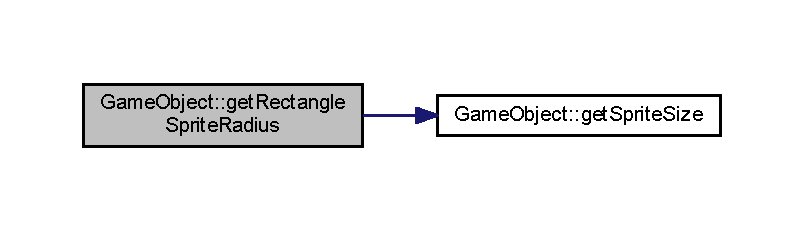
\includegraphics[width=350pt]{class_game_object_a8220201988f2aaea8a6f748872e188a9_cgraph}
\end{center}
\end{figure}




Here is the caller graph for this function\+:\nopagebreak
\begin{figure}[H]
\begin{center}
\leavevmode
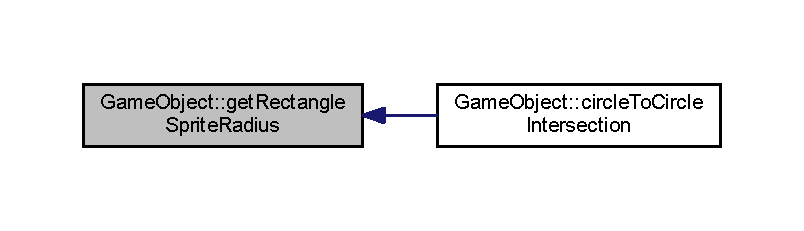
\includegraphics[width=350pt]{class_game_object_a8220201988f2aaea8a6f748872e188a9_icgraph}
\end{center}
\end{figure}


\hypertarget{class_game_object_ad6d60e0c273cb0074c91a19f3aed8708}{\index{Game\+Object@{Game\+Object}!get\+Sprite\+Center@{get\+Sprite\+Center}}
\index{get\+Sprite\+Center@{get\+Sprite\+Center}!Game\+Object@{Game\+Object}}
\subsubsection[{get\+Sprite\+Center}]{\setlength{\rightskip}{0pt plus 5cm}std\+::pair$<$ float, float $>$ Game\+Object\+::get\+Sprite\+Center (
\begin{DoxyParamCaption}
{}
\end{DoxyParamCaption}
)\hspace{0.3cm}{\ttfamily [virtual]}}}\label{class_game_object_ad6d60e0c273cb0074c91a19f3aed8708}


Gets the center of a sprite. 

\begin{DoxyReturn}{Returns}
std\+::pair$<$float, float$>$ 
\end{DoxyReturn}


Here is the caller graph for this function\+:
\nopagebreak
\begin{figure}[H]
\begin{center}
\leavevmode
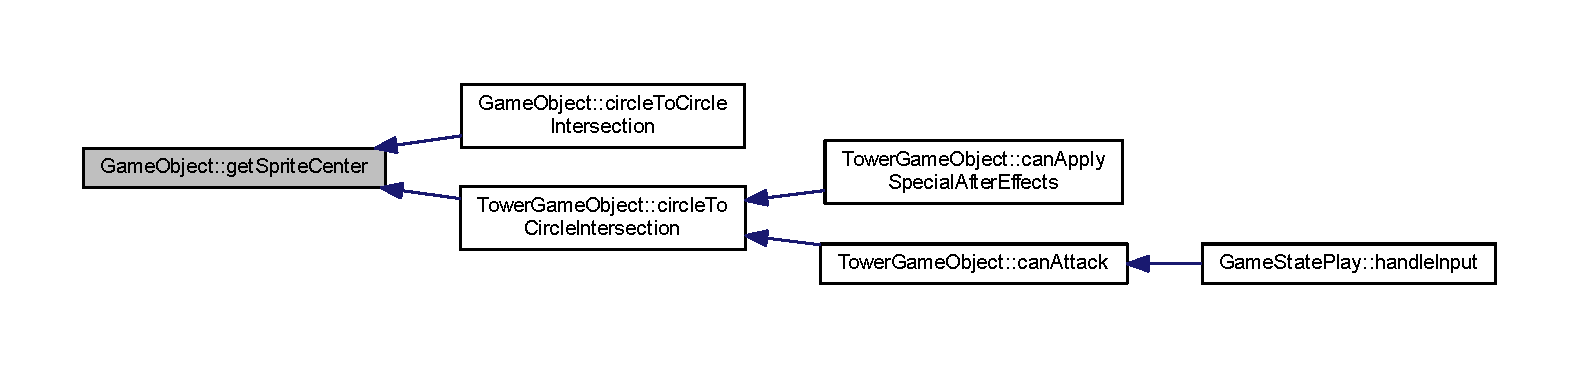
\includegraphics[width=350pt]{class_game_object_ad6d60e0c273cb0074c91a19f3aed8708_icgraph}
\end{center}
\end{figure}


\hypertarget{class_game_object_a3731c03ddcbdb904bd41af78e09d262a}{\index{Game\+Object@{Game\+Object}!get\+Sprite\+Size@{get\+Sprite\+Size}}
\index{get\+Sprite\+Size@{get\+Sprite\+Size}!Game\+Object@{Game\+Object}}
\subsubsection[{get\+Sprite\+Size}]{\setlength{\rightskip}{0pt plus 5cm}std\+::pair$<$ float, float $>$ Game\+Object\+::get\+Sprite\+Size (
\begin{DoxyParamCaption}
{}
\end{DoxyParamCaption}
)\hspace{0.3cm}{\ttfamily [virtual]}}}\label{class_game_object_a3731c03ddcbdb904bd41af78e09d262a}


Gets the size of a sprite. 

\begin{DoxyReturn}{Returns}
std\+::pair$<$float, float$>$ 
\end{DoxyReturn}


Here is the caller graph for this function\+:
\nopagebreak
\begin{figure}[H]
\begin{center}
\leavevmode
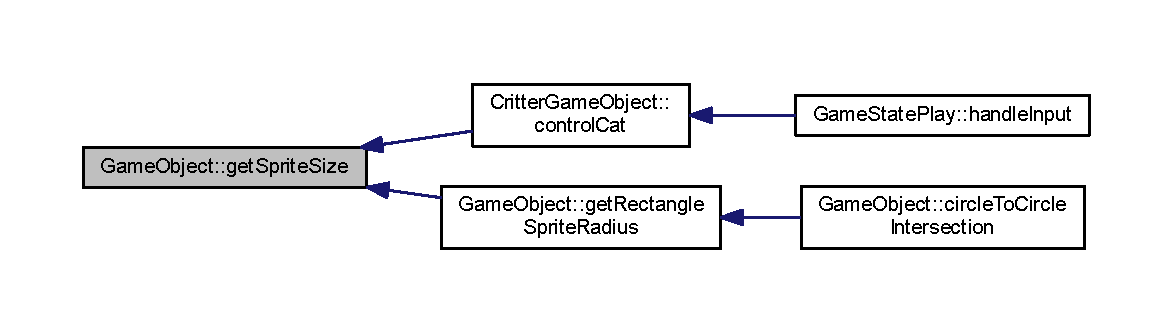
\includegraphics[width=350pt]{class_game_object_a3731c03ddcbdb904bd41af78e09d262a_icgraph}
\end{center}
\end{figure}


\hypertarget{class_game_object_acc593e5b75a58c4a59ad59da654ce807}{\index{Game\+Object@{Game\+Object}!load@{load}}
\index{load@{load}!Game\+Object@{Game\+Object}}
\subsubsection[{load}]{\setlength{\rightskip}{0pt plus 5cm}void Game\+Object\+::load (
\begin{DoxyParamCaption}
\item[{std\+::string}]{file\+\_\+name}
\end{DoxyParamCaption}
)\hspace{0.3cm}{\ttfamily [virtual]}}}\label{class_game_object_acc593e5b75a58c4a59ad59da654ce807}


Loads a texture using the \hyperlink{class_texture_manager}{Texture\+Manager} class and creates a sprite. 


\begin{DoxyParams}{Parameters}
{\em file\+\_\+name} & The file name of the texture that is being loaded. \\
\hline
\end{DoxyParams}
\begin{DoxyReturn}{Returns}
Void.
\end{DoxyReturn}
\hyperlink{class_game_object_acc593e5b75a58c4a59ad59da654ce807}{load()} gets a reference to the \hyperlink{class_texture_manager}{Texture\+Manager} instance, loads the texture based on the given file name, sets the texture for the \hyperlink{class_game_object}{Game\+Object} sprite, and indicates that the sprite creation is true. 

Here is the call graph for this function\+:\nopagebreak
\begin{figure}[H]
\begin{center}
\leavevmode
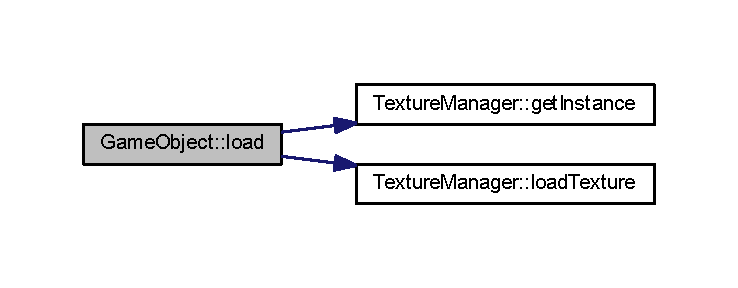
\includegraphics[width=350pt]{class_game_object_acc593e5b75a58c4a59ad59da654ce807_cgraph}
\end{center}
\end{figure}




Here is the caller graph for this function\+:
\nopagebreak
\begin{figure}[H]
\begin{center}
\leavevmode
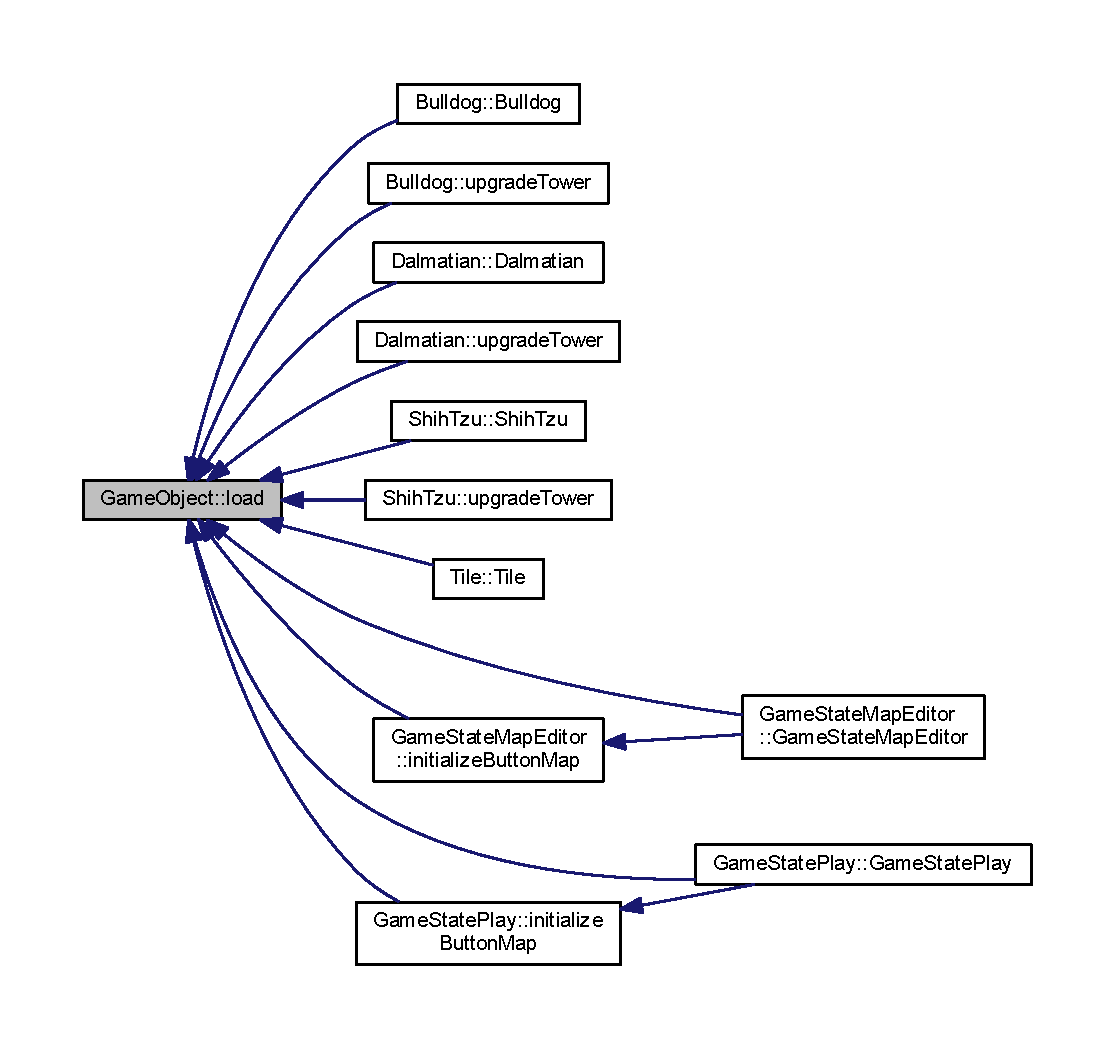
\includegraphics[height=550pt]{class_game_object_acc593e5b75a58c4a59ad59da654ce807_icgraph}
\end{center}
\end{figure}


\hypertarget{class_game_object_a6fa0d948eccbd0345cda6bdea5b5196a}{\index{Game\+Object@{Game\+Object}!move@{move}}
\index{move@{move}!Game\+Object@{Game\+Object}}
\subsubsection[{move}]{\setlength{\rightskip}{0pt plus 5cm}void Game\+Object\+::move (
\begin{DoxyParamCaption}
\item[{float}]{x, }
\item[{float}]{y}
\end{DoxyParamCaption}
)\hspace{0.3cm}{\ttfamily [virtual]}}}\label{class_game_object_a6fa0d948eccbd0345cda6bdea5b5196a}
\hypertarget{class_game_object_a3ad77a6b8bc1adfb8ea463f12c022b1e}{\index{Game\+Object@{Game\+Object}!move@{move}}
\index{move@{move}!Game\+Object@{Game\+Object}}
\subsubsection[{move}]{\setlength{\rightskip}{0pt plus 5cm}void Game\+Object\+::move (
\begin{DoxyParamCaption}
\item[{const sf\+::\+Vector2f \&}]{offset}
\end{DoxyParamCaption}
)\hspace{0.3cm}{\ttfamily [virtual]}}}\label{class_game_object_a3ad77a6b8bc1adfb8ea463f12c022b1e}
\hypertarget{class_game_object_a180d6e9e7afa44b30ca678a95c6f4dad}{\index{Game\+Object@{Game\+Object}!set\+Position@{set\+Position}}
\index{set\+Position@{set\+Position}!Game\+Object@{Game\+Object}}
\subsubsection[{set\+Position}]{\setlength{\rightskip}{0pt plus 5cm}void Game\+Object\+::set\+Position (
\begin{DoxyParamCaption}
\item[{float}]{x, }
\item[{float}]{y}
\end{DoxyParamCaption}
)\hspace{0.3cm}{\ttfamily [virtual]}}}\label{class_game_object_a180d6e9e7afa44b30ca678a95c6f4dad}


Sets the initial draw position of a \hyperlink{class_game_object}{Game\+Object} instance. 


\begin{DoxyParams}{Parameters}
{\em x} & X-\/coordinate of the position. \\
\hline
\end{DoxyParams}
\begin{DoxyReturn}{Returns}
Void.
\end{DoxyReturn}
\hyperlink{class_game_object_a180d6e9e7afa44b30ca678a95c6f4dad}{set\+Position()} sets x and y coordinates of the sprite if it has been created. 

Here is the caller graph for this function\+:
\nopagebreak
\begin{figure}[H]
\begin{center}
\leavevmode
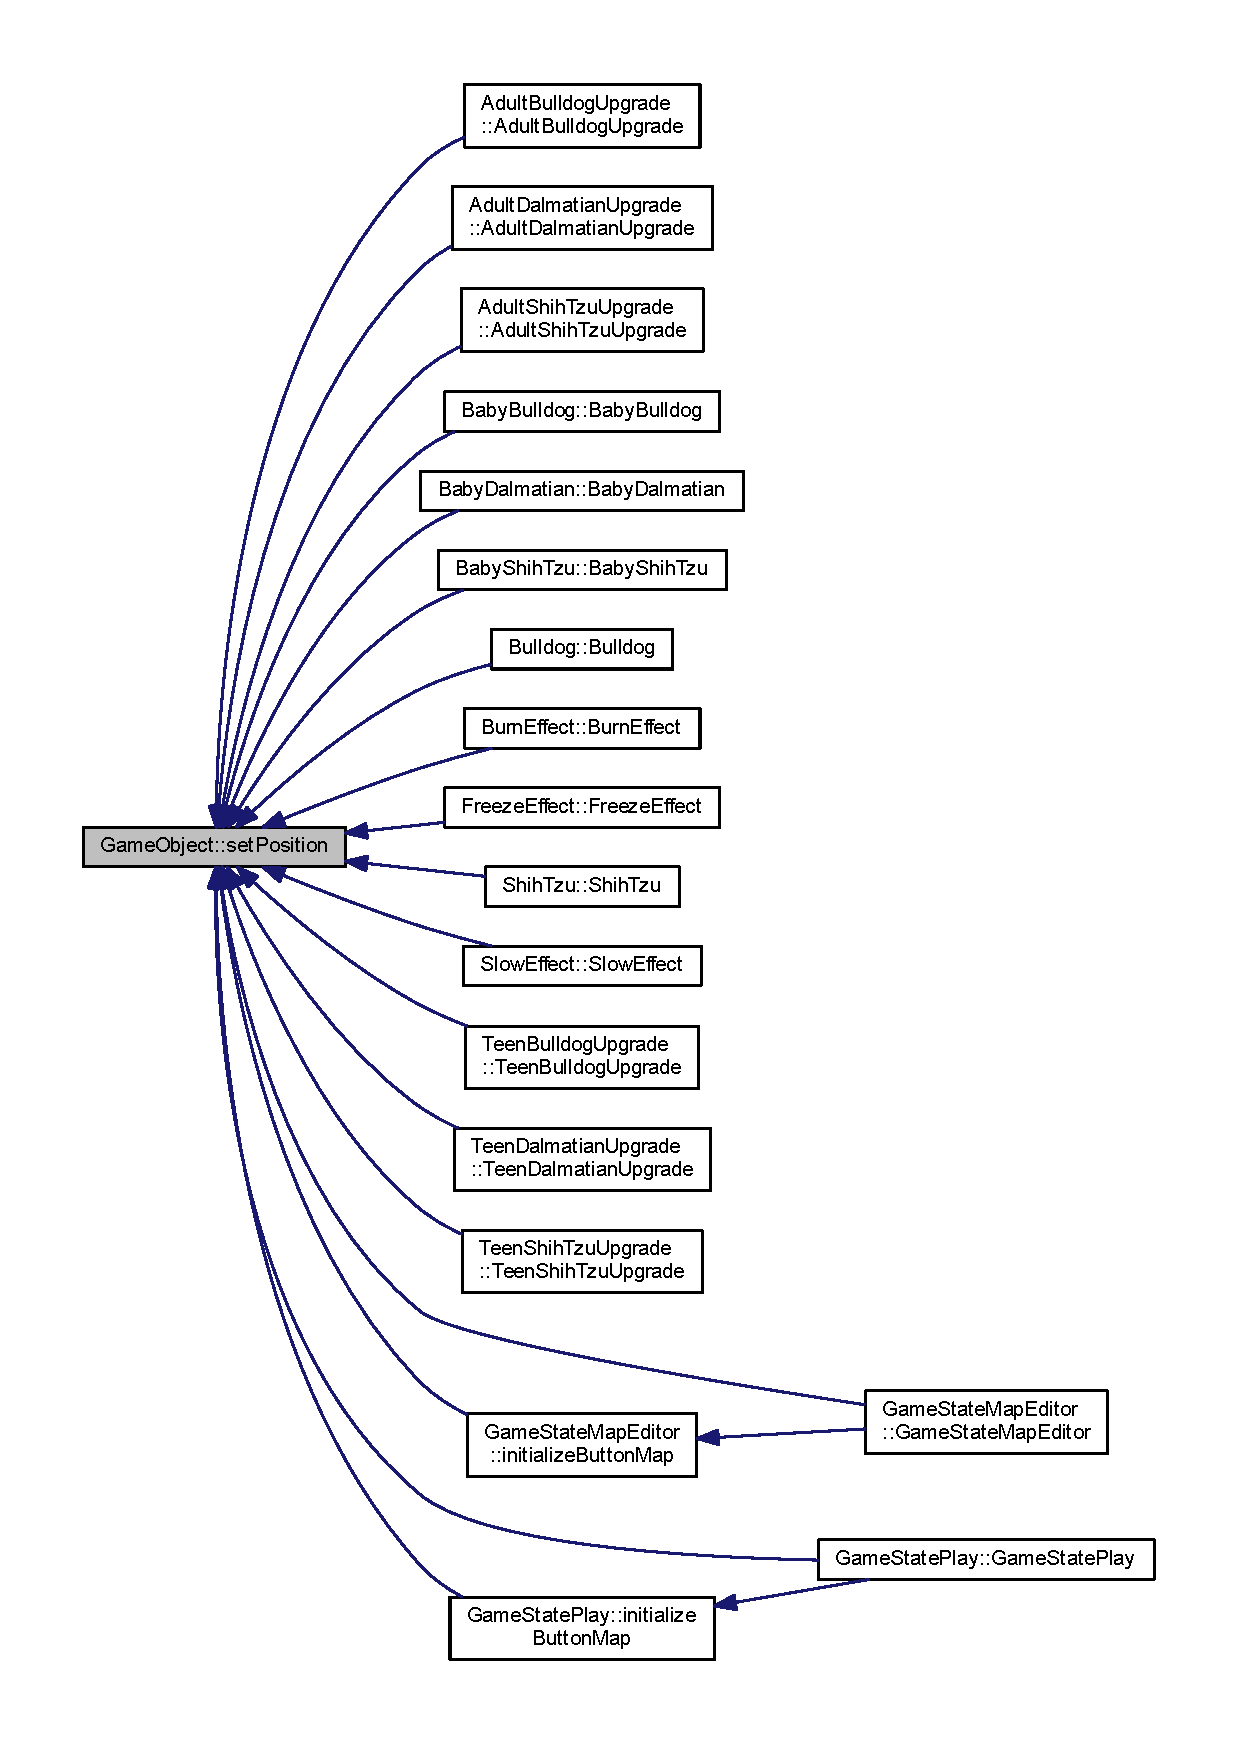
\includegraphics[width=350pt]{class_game_object_a180d6e9e7afa44b30ca678a95c6f4dad_icgraph}
\end{center}
\end{figure}


\hypertarget{class_game_object_a320a94559557834d53bffa538d8349c9}{\index{Game\+Object@{Game\+Object}!set\+Rotation@{set\+Rotation}}
\index{set\+Rotation@{set\+Rotation}!Game\+Object@{Game\+Object}}
\subsubsection[{set\+Rotation}]{\setlength{\rightskip}{0pt plus 5cm}void Game\+Object\+::set\+Rotation (
\begin{DoxyParamCaption}
\item[{float}]{angle}
\end{DoxyParamCaption}
)\hspace{0.3cm}{\ttfamily [virtual]}}}\label{class_game_object_a320a94559557834d53bffa538d8349c9}


Here is the caller graph for this function\+:\nopagebreak
\begin{figure}[H]
\begin{center}
\leavevmode
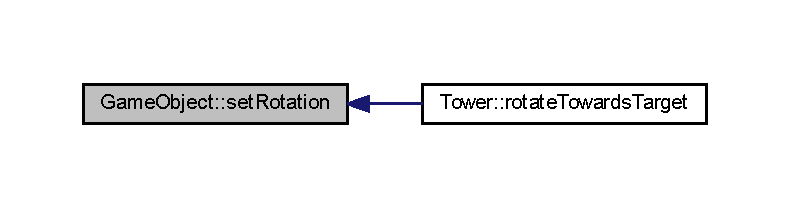
\includegraphics[width=350pt]{class_game_object_a320a94559557834d53bffa538d8349c9_icgraph}
\end{center}
\end{figure}


\hypertarget{class_game_object_adf7e04407f7c2a5bd487b459efe9fd79}{\index{Game\+Object@{Game\+Object}!sprite\+Contains@{sprite\+Contains}}
\index{sprite\+Contains@{sprite\+Contains}!Game\+Object@{Game\+Object}}
\subsubsection[{sprite\+Contains}]{\setlength{\rightskip}{0pt plus 5cm}bool Game\+Object\+::sprite\+Contains (
\begin{DoxyParamCaption}
\item[{sf\+::\+Vector2i}]{position}
\end{DoxyParamCaption}
) const}}\label{class_game_object_adf7e04407f7c2a5bd487b459efe9fd79}


Here is the caller graph for this function\+:\nopagebreak
\begin{figure}[H]
\begin{center}
\leavevmode
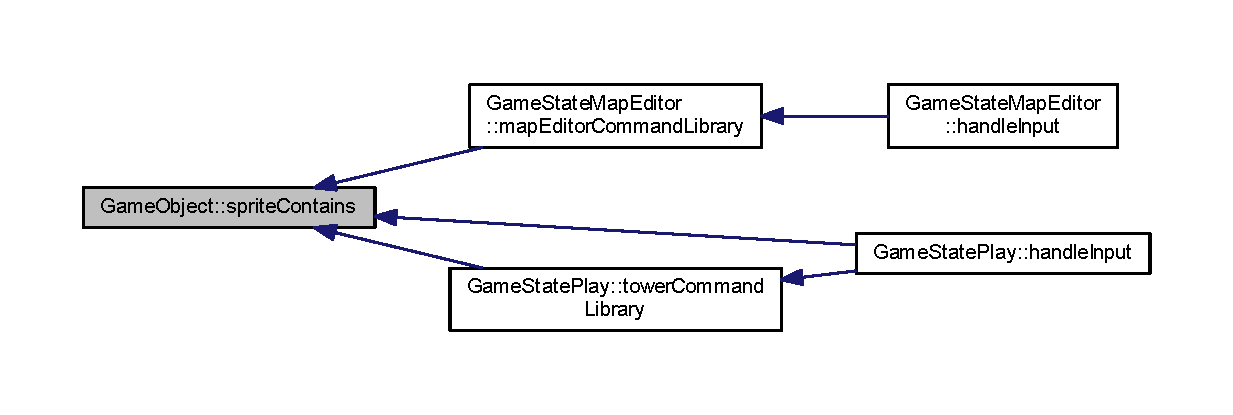
\includegraphics[width=350pt]{class_game_object_adf7e04407f7c2a5bd487b459efe9fd79_icgraph}
\end{center}
\end{figure}




\subsection{Member Data Documentation}
\hypertarget{class_game_object_a1b725daa9c79833a7139469468dc770a}{\index{Game\+Object@{Game\+Object}!file\+\_\+name@{file\+\_\+name}}
\index{file\+\_\+name@{file\+\_\+name}!Game\+Object@{Game\+Object}}
\subsubsection[{file\+\_\+name}]{\setlength{\rightskip}{0pt plus 5cm}std\+::string Game\+Object\+::file\+\_\+name\hspace{0.3cm}{\ttfamily [protected]}}}\label{class_game_object_a1b725daa9c79833a7139469468dc770a}


The file name of the sprite's texture. 

\hypertarget{class_game_object_a677286bcb906871b6a3eb0c0b9342176}{\index{Game\+Object@{Game\+Object}!is\+Sprite\+Created@{is\+Sprite\+Created}}
\index{is\+Sprite\+Created@{is\+Sprite\+Created}!Game\+Object@{Game\+Object}}
\subsubsection[{is\+Sprite\+Created}]{\setlength{\rightskip}{0pt plus 5cm}bool Game\+Object\+::is\+Sprite\+Created\hspace{0.3cm}{\ttfamily [protected]}}}\label{class_game_object_a677286bcb906871b6a3eb0c0b9342176}


Boolean indicating whether or not a sprite has been created. The purpose of this bool is to ensure that the sprite exists before the class attempts to draw the \hyperlink{class_game_object}{Game\+Object}. 

\hypertarget{class_game_object_a86e4253e3734436b4a5a0c503e0033b4}{\index{Game\+Object@{Game\+Object}!position@{position}}
\index{position@{position}!Game\+Object@{Game\+Object}}
\subsubsection[{position}]{\setlength{\rightskip}{0pt plus 5cm}sf\+::\+Vector2f Game\+Object\+::position\hspace{0.3cm}{\ttfamily [protected]}}}\label{class_game_object_a86e4253e3734436b4a5a0c503e0033b4}
\hypertarget{class_game_object_abb3608f1c76edd590e023585c2216f02}{\index{Game\+Object@{Game\+Object}!sprite@{sprite}}
\index{sprite@{sprite}!Game\+Object@{Game\+Object}}
\subsubsection[{sprite}]{\setlength{\rightskip}{0pt plus 5cm}sf\+::\+Sprite Game\+Object\+::sprite\hspace{0.3cm}{\ttfamily [protected]}}}\label{class_game_object_abb3608f1c76edd590e023585c2216f02}


The Sprite instance of the \hyperlink{class_game_object}{Game\+Object}. 



The documentation for this class was generated from the following files\+:\begin{DoxyCompactItemize}
\item 
jamms/\+Tower\+Defense/\+Tower\+Defense/include/game\+Objects/\hyperlink{_game_object_8h}{Game\+Object.\+h}\item 
jamms/\+Tower\+Defense/\+Tower\+Defense/src/game\+Objects/\hyperlink{_game_object_8cpp}{Game\+Object.\+cpp}\end{DoxyCompactItemize}

\hypertarget{struct_game_object_manager_1_1_game_object_deallocator}{\section{Game\+Object\+Manager\+:\+:Game\+Object\+Deallocator Struct Reference}
\label{struct_game_object_manager_1_1_game_object_deallocator}\index{Game\+Object\+Manager\+::\+Game\+Object\+Deallocator@{Game\+Object\+Manager\+::\+Game\+Object\+Deallocator}}
}


Collaboration diagram for Game\+Object\+Manager\+:\+:Game\+Object\+Deallocator\+:\nopagebreak
\begin{figure}[H]
\begin{center}
\leavevmode
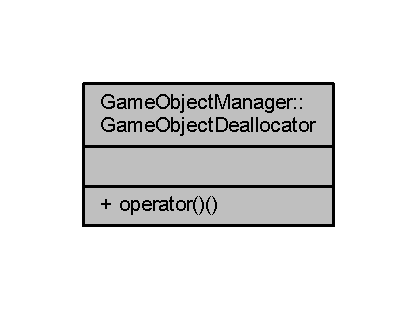
\includegraphics[width=200pt]{struct_game_object_manager_1_1_game_object_deallocator__coll__graph}
\end{center}
\end{figure}
\subsection*{Public Member Functions}
\begin{DoxyCompactItemize}
\item 
void \hyperlink{struct_game_object_manager_1_1_game_object_deallocator_a7fe3b540a7ac235e0d5b95c9f865db36}{operator()} (const std\+::pair$<$ std\+::string, \hyperlink{class_game_object}{Game\+Object} $\ast$ $>$ \&p) const 
\end{DoxyCompactItemize}


\subsection{Member Function Documentation}
\hypertarget{struct_game_object_manager_1_1_game_object_deallocator_a7fe3b540a7ac235e0d5b95c9f865db36}{\index{Game\+Object\+Manager\+::\+Game\+Object\+Deallocator@{Game\+Object\+Manager\+::\+Game\+Object\+Deallocator}!operator()@{operator()}}
\index{operator()@{operator()}!Game\+Object\+Manager\+::\+Game\+Object\+Deallocator@{Game\+Object\+Manager\+::\+Game\+Object\+Deallocator}}
\subsubsection[{operator()}]{\setlength{\rightskip}{0pt plus 5cm}void Game\+Object\+Manager\+::\+Game\+Object\+Deallocator\+::operator() (
\begin{DoxyParamCaption}
\item[{const std\+::pair$<$ std\+::string, {\bf Game\+Object} $\ast$ $>$ \&}]{p}
\end{DoxyParamCaption}
) const\hspace{0.3cm}{\ttfamily [inline]}}}\label{struct_game_object_manager_1_1_game_object_deallocator_a7fe3b540a7ac235e0d5b95c9f865db36}


The documentation for this struct was generated from the following file\+:\begin{DoxyCompactItemize}
\item 
jamms/\+Tower\+Defense/\+Tower\+Defense/include/managers/\hyperlink{_game_object_manager_8h}{Game\+Object\+Manager.\+h}\end{DoxyCompactItemize}

\hypertarget{class_game_object_manager}{\section{Game\+Object\+Manager Class Reference}
\label{class_game_object_manager}\index{Game\+Object\+Manager@{Game\+Object\+Manager}}
}


{\ttfamily \#include $<$Game\+Object\+Manager.\+h$>$}



Collaboration diagram for Game\+Object\+Manager\+:
\nopagebreak
\begin{figure}[H]
\begin{center}
\leavevmode
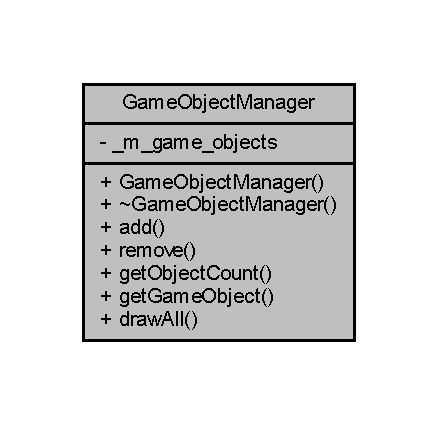
\includegraphics[width=210pt]{class_game_object_manager__coll__graph}
\end{center}
\end{figure}
\subsection*{Classes}
\begin{DoxyCompactItemize}
\item 
struct \hyperlink{struct_game_object_manager_1_1_game_object_deallocator}{Game\+Object\+Deallocator}
\end{DoxyCompactItemize}
\subsection*{Public Member Functions}
\begin{DoxyCompactItemize}
\item 
\hyperlink{class_game_object_manager_a58cbaec4182cda7c6d48eef7b14885e8}{Game\+Object\+Manager} ()
\item 
\hyperlink{class_game_object_manager_a91d57baff47ce5090e5e4590f531051d}{$\sim$\+Game\+Object\+Manager} ()
\item 
void \hyperlink{class_game_object_manager_abd5bf89a1a767486dbcb0ef1a600d0b2}{add} (std\+::string name, \hyperlink{class_game_object}{Game\+Object} $\ast$game\+\_\+object)
\item 
void \hyperlink{class_game_object_manager_a0469ca3148149a6cfa0214a0f4f4b102}{remove} (std\+::string name)
\item 
int \hyperlink{class_game_object_manager_aea3ab827dd015aae7a8e8d53fdd6d2b5}{get\+Object\+Count} () const 
\item 
\hyperlink{class_game_object}{Game\+Object} $\ast$ \hyperlink{class_game_object_manager_a9711a8874ef5581db4832fc28dc0e87c}{get\+Game\+Object} (std\+::string name) const 
\item 
void \hyperlink{class_game_object_manager_a7ab22ae52c51eba926aa461028c00fb3}{draw\+All} (sf\+::\+Render\+Window \&render\+\_\+window)
\end{DoxyCompactItemize}
\subsection*{Private Attributes}
\begin{DoxyCompactItemize}
\item 
std\+::map$<$ std\+::string, \\*
\hyperlink{class_game_object}{Game\+Object} $\ast$ $>$ \hyperlink{class_game_object_manager_a8e5f1dadc41529ca112ff4aa23d92048}{\+\_\+m\+\_\+game\+\_\+objects}
\end{DoxyCompactItemize}


\subsection{Constructor \& Destructor Documentation}
\hypertarget{class_game_object_manager_a58cbaec4182cda7c6d48eef7b14885e8}{\index{Game\+Object\+Manager@{Game\+Object\+Manager}!Game\+Object\+Manager@{Game\+Object\+Manager}}
\index{Game\+Object\+Manager@{Game\+Object\+Manager}!Game\+Object\+Manager@{Game\+Object\+Manager}}
\subsubsection[{Game\+Object\+Manager}]{\setlength{\rightskip}{0pt plus 5cm}Game\+Object\+Manager\+::\+Game\+Object\+Manager (
\begin{DoxyParamCaption}
{}
\end{DoxyParamCaption}
)\hspace{0.3cm}{\ttfamily [inline]}}}\label{class_game_object_manager_a58cbaec4182cda7c6d48eef7b14885e8}
\hypertarget{class_game_object_manager_a91d57baff47ce5090e5e4590f531051d}{\index{Game\+Object\+Manager@{Game\+Object\+Manager}!````~Game\+Object\+Manager@{$\sim$\+Game\+Object\+Manager}}
\index{````~Game\+Object\+Manager@{$\sim$\+Game\+Object\+Manager}!Game\+Object\+Manager@{Game\+Object\+Manager}}
\subsubsection[{$\sim$\+Game\+Object\+Manager}]{\setlength{\rightskip}{0pt plus 5cm}Game\+Object\+Manager\+::$\sim$\+Game\+Object\+Manager (
\begin{DoxyParamCaption}
{}
\end{DoxyParamCaption}
)}}\label{class_game_object_manager_a91d57baff47ce5090e5e4590f531051d}


\subsection{Member Function Documentation}
\hypertarget{class_game_object_manager_abd5bf89a1a767486dbcb0ef1a600d0b2}{\index{Game\+Object\+Manager@{Game\+Object\+Manager}!add@{add}}
\index{add@{add}!Game\+Object\+Manager@{Game\+Object\+Manager}}
\subsubsection[{add}]{\setlength{\rightskip}{0pt plus 5cm}void Game\+Object\+Manager\+::add (
\begin{DoxyParamCaption}
\item[{std\+::string}]{name, }
\item[{{\bf Game\+Object} $\ast$}]{game\+\_\+object}
\end{DoxyParamCaption}
)}}\label{class_game_object_manager_abd5bf89a1a767486dbcb0ef1a600d0b2}
\hypertarget{class_game_object_manager_a7ab22ae52c51eba926aa461028c00fb3}{\index{Game\+Object\+Manager@{Game\+Object\+Manager}!draw\+All@{draw\+All}}
\index{draw\+All@{draw\+All}!Game\+Object\+Manager@{Game\+Object\+Manager}}
\subsubsection[{draw\+All}]{\setlength{\rightskip}{0pt plus 5cm}void Game\+Object\+Manager\+::draw\+All (
\begin{DoxyParamCaption}
\item[{sf\+::\+Render\+Window \&}]{render\+\_\+window}
\end{DoxyParamCaption}
)}}\label{class_game_object_manager_a7ab22ae52c51eba926aa461028c00fb3}
\hypertarget{class_game_object_manager_a9711a8874ef5581db4832fc28dc0e87c}{\index{Game\+Object\+Manager@{Game\+Object\+Manager}!get\+Game\+Object@{get\+Game\+Object}}
\index{get\+Game\+Object@{get\+Game\+Object}!Game\+Object\+Manager@{Game\+Object\+Manager}}
\subsubsection[{get\+Game\+Object}]{\setlength{\rightskip}{0pt plus 5cm}{\bf Game\+Object} $\ast$ Game\+Object\+Manager\+::get\+Game\+Object (
\begin{DoxyParamCaption}
\item[{std\+::string}]{name}
\end{DoxyParamCaption}
) const}}\label{class_game_object_manager_a9711a8874ef5581db4832fc28dc0e87c}
\hypertarget{class_game_object_manager_aea3ab827dd015aae7a8e8d53fdd6d2b5}{\index{Game\+Object\+Manager@{Game\+Object\+Manager}!get\+Object\+Count@{get\+Object\+Count}}
\index{get\+Object\+Count@{get\+Object\+Count}!Game\+Object\+Manager@{Game\+Object\+Manager}}
\subsubsection[{get\+Object\+Count}]{\setlength{\rightskip}{0pt plus 5cm}int Game\+Object\+Manager\+::get\+Object\+Count (
\begin{DoxyParamCaption}
{}
\end{DoxyParamCaption}
) const}}\label{class_game_object_manager_aea3ab827dd015aae7a8e8d53fdd6d2b5}
\hypertarget{class_game_object_manager_a0469ca3148149a6cfa0214a0f4f4b102}{\index{Game\+Object\+Manager@{Game\+Object\+Manager}!remove@{remove}}
\index{remove@{remove}!Game\+Object\+Manager@{Game\+Object\+Manager}}
\subsubsection[{remove}]{\setlength{\rightskip}{0pt plus 5cm}void Game\+Object\+Manager\+::remove (
\begin{DoxyParamCaption}
\item[{std\+::string}]{name}
\end{DoxyParamCaption}
)}}\label{class_game_object_manager_a0469ca3148149a6cfa0214a0f4f4b102}


\subsection{Member Data Documentation}
\hypertarget{class_game_object_manager_a8e5f1dadc41529ca112ff4aa23d92048}{\index{Game\+Object\+Manager@{Game\+Object\+Manager}!\+\_\+m\+\_\+game\+\_\+objects@{\+\_\+m\+\_\+game\+\_\+objects}}
\index{\+\_\+m\+\_\+game\+\_\+objects@{\+\_\+m\+\_\+game\+\_\+objects}!Game\+Object\+Manager@{Game\+Object\+Manager}}
\subsubsection[{\+\_\+m\+\_\+game\+\_\+objects}]{\setlength{\rightskip}{0pt plus 5cm}std\+::map$<$std\+::string, {\bf Game\+Object}$\ast$$>$ Game\+Object\+Manager\+::\+\_\+m\+\_\+game\+\_\+objects\hspace{0.3cm}{\ttfamily [private]}}}\label{class_game_object_manager_a8e5f1dadc41529ca112ff4aa23d92048}


The documentation for this class was generated from the following files\+:\begin{DoxyCompactItemize}
\item 
jamms/\+Tower\+Defense/\+Tower\+Defense/include/managers/\hyperlink{_game_object_manager_8h}{Game\+Object\+Manager.\+h}\item 
jamms/\+Tower\+Defense/\+Tower\+Defense/src/managers/\hyperlink{_game_object_manager_8cpp}{Game\+Object\+Manager.\+cpp}\end{DoxyCompactItemize}

\hypertarget{class_game_state}{\section{Game\+State Class Reference}
\label{class_game_state}\index{Game\+State@{Game\+State}}
}


\hyperlink{class_game_state}{Game\+State} virtual base class. \hyperlink{class_game_state}{Game\+State} is an interface for states within the game.  




{\ttfamily \#include $<$Game\+State.\+h$>$}



Inheritance diagram for Game\+State\+:
\nopagebreak
\begin{figure}[H]
\begin{center}
\leavevmode
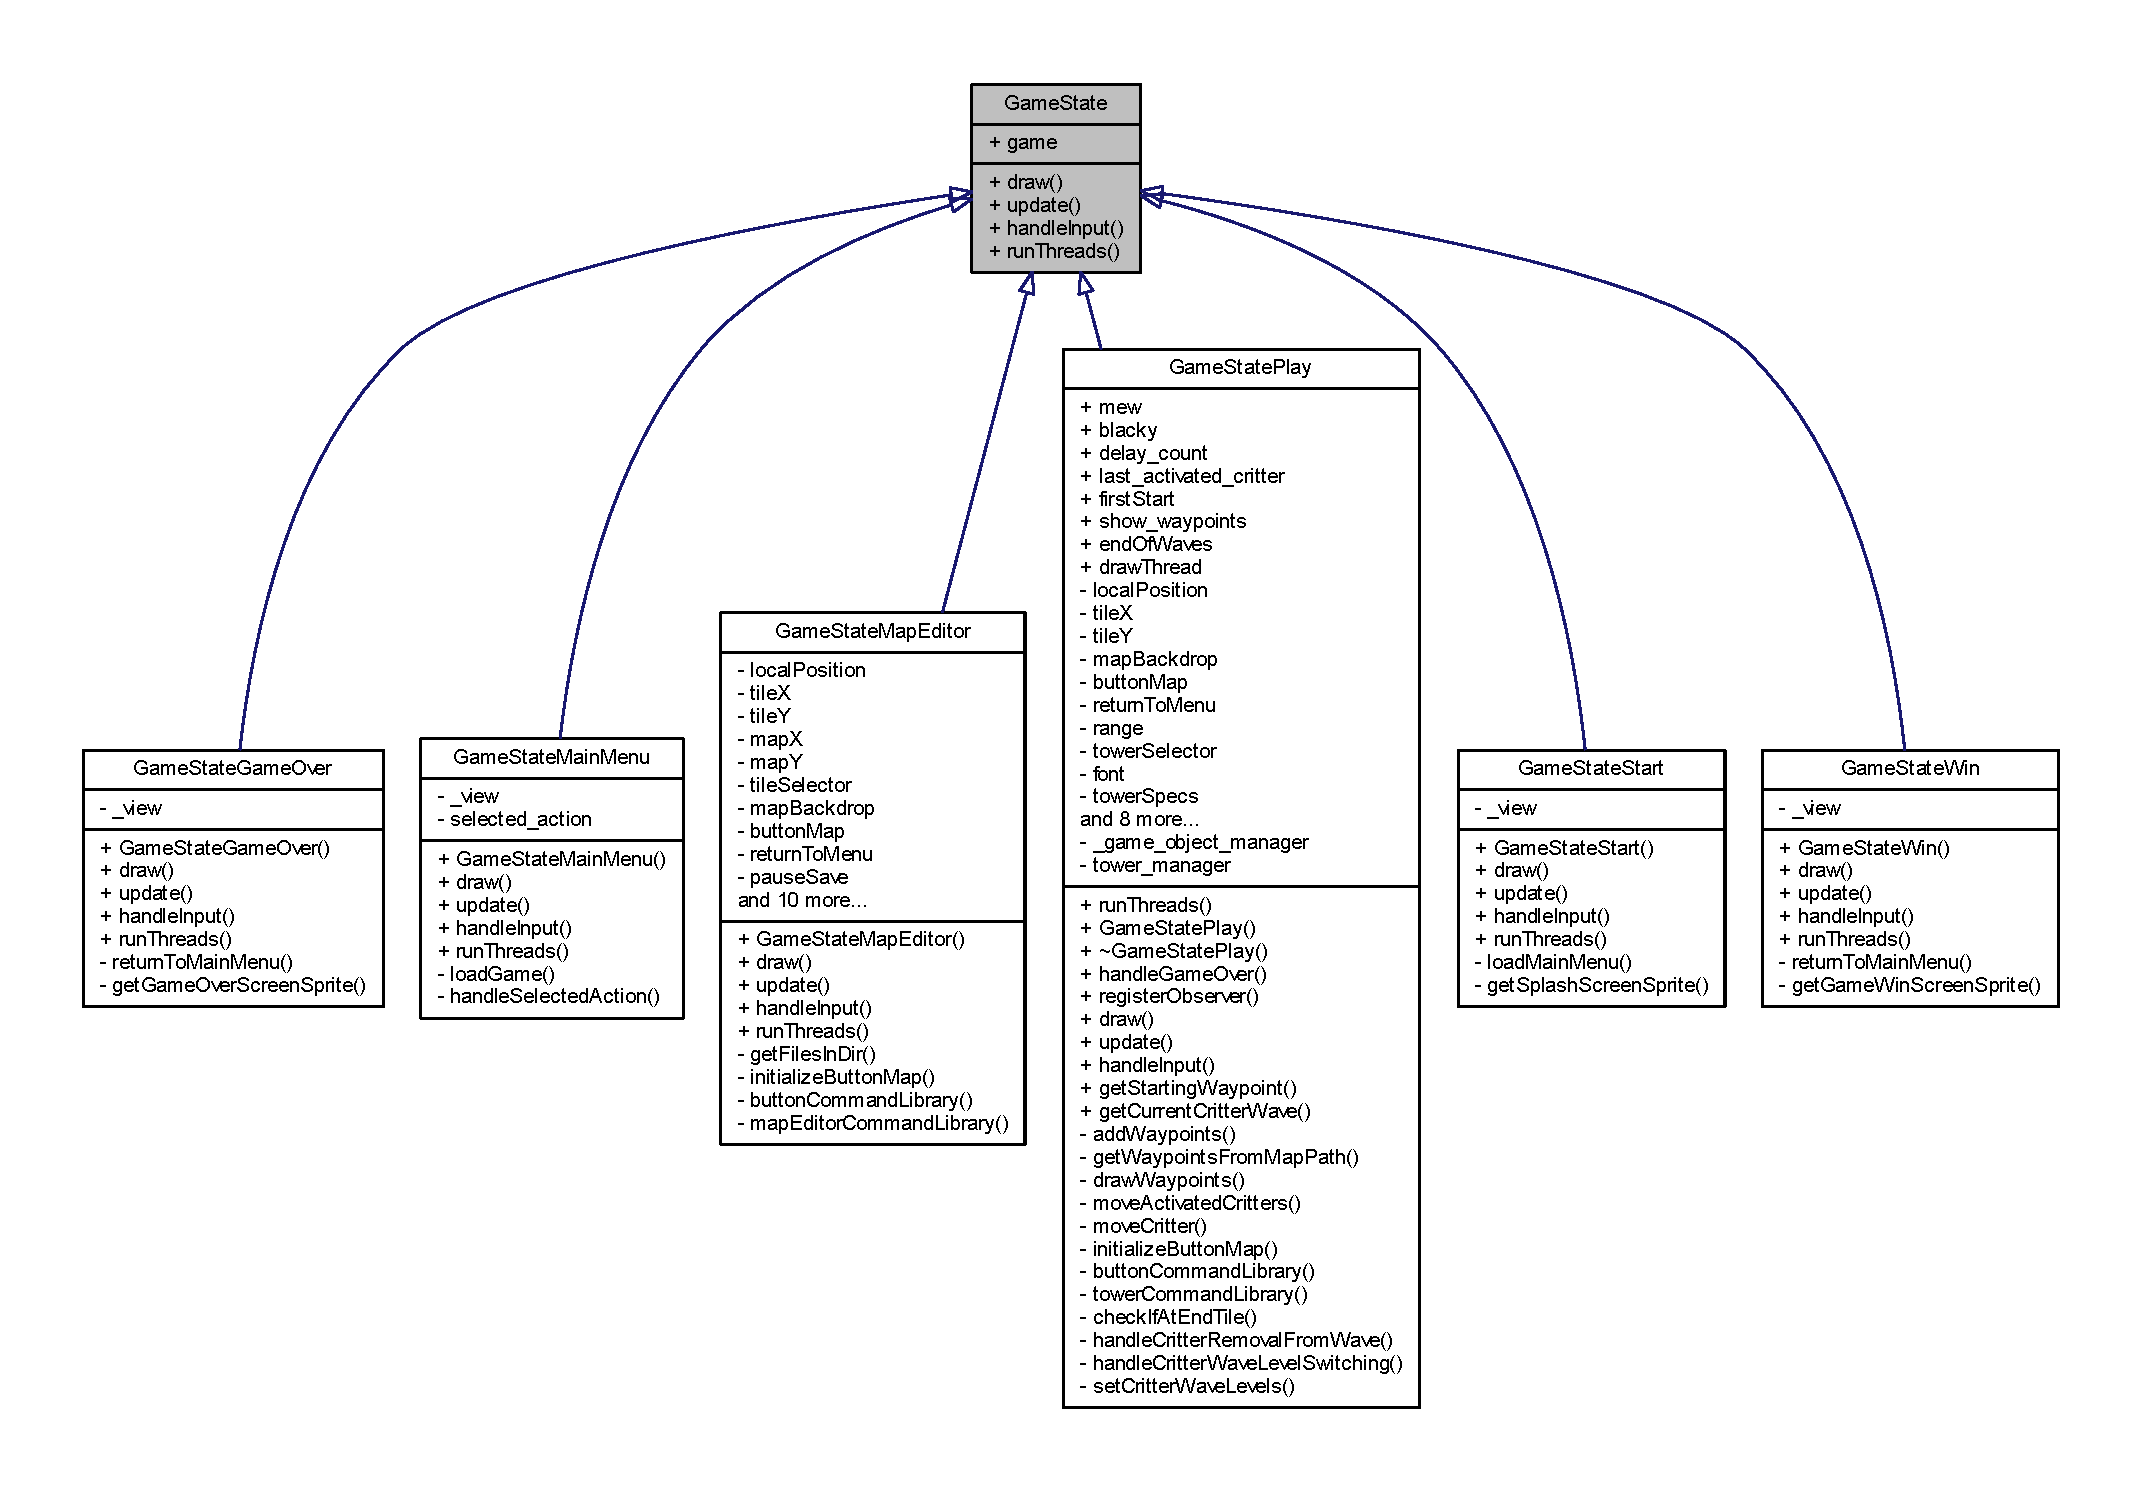
\includegraphics[width=350pt]{class_game_state__inherit__graph}
\end{center}
\end{figure}


Collaboration diagram for Game\+State\+:
\nopagebreak
\begin{figure}[H]
\begin{center}
\leavevmode
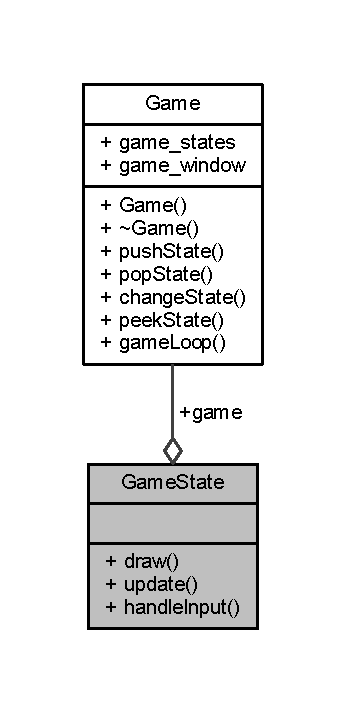
\includegraphics[width=350pt]{class_game_state__coll__graph}
\end{center}
\end{figure}
\subsection*{Public Member Functions}
\begin{DoxyCompactItemize}
\item 
virtual void \hyperlink{class_game_state_a55a6a68aabdf7054ea0e6ddbf24902df}{draw} (const float delta\+\_\+time)=0
\item 
virtual void \hyperlink{class_game_state_ad331d02d3989271b8cbc88fcb1448959}{update} (const float delta\+\_\+time)=0
\item 
virtual void \hyperlink{class_game_state_a970b55edd5a1da31ea0f7113e2c1f85a}{handle\+Input} ()=0
\item 
virtual void \hyperlink{class_game_state_a98cd49f1d8fd9fc3e79d607a238ba518}{run\+Threads} ()=0
\end{DoxyCompactItemize}
\subsection*{Public Attributes}
\begin{DoxyCompactItemize}
\item 
\hyperlink{class_game}{Game} $\ast$ \hyperlink{class_game_state_a355a79415b9ef63c2aec1448a99f6e71}{game}
\begin{DoxyCompactList}\small\item\em Pointer to \hyperlink{class_game}{Game} instance that handles the changing. of the states and store the info in every game state. \end{DoxyCompactList}\end{DoxyCompactItemize}


\subsection{Detailed Description}
\hyperlink{class_game_state}{Game\+State} virtual base class. \hyperlink{class_game_state}{Game\+State} is an interface for states within the game. 

\subsection{Member Function Documentation}
\hypertarget{class_game_state_a55a6a68aabdf7054ea0e6ddbf24902df}{\index{Game\+State@{Game\+State}!draw@{draw}}
\index{draw@{draw}!Game\+State@{Game\+State}}
\subsubsection[{draw}]{\setlength{\rightskip}{0pt plus 5cm}virtual void Game\+State\+::draw (
\begin{DoxyParamCaption}
\item[{const float}]{delta\+\_\+time}
\end{DoxyParamCaption}
)\hspace{0.3cm}{\ttfamily [pure virtual]}}}\label{class_game_state_a55a6a68aabdf7054ea0e6ddbf24902df}


Implemented in \hyperlink{class_game_state_play_a63a3ba0c891afd8ec126806bab4f315a}{Game\+State\+Play}, \hyperlink{class_game_state_map_editor_a37c87643309459ac32d0b5f608bc93b0}{Game\+State\+Map\+Editor}, \hyperlink{class_game_state_main_menu_ad34efc1ade7193ce765d00ac60f019ed}{Game\+State\+Main\+Menu}, \hyperlink{class_game_state_game_over_a1e88ff4cbd7d608858604efdb16e2adc}{Game\+State\+Game\+Over}, \hyperlink{class_game_state_start_a0969e5227b6f2eaabd53ee69f32a37e7}{Game\+State\+Start}, and \hyperlink{class_game_state_win_aa5d3bc751d492439016f8d42fce2110a}{Game\+State\+Win}.



Here is the caller graph for this function\+:
\nopagebreak
\begin{figure}[H]
\begin{center}
\leavevmode
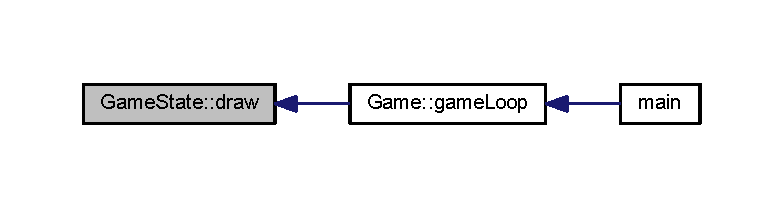
\includegraphics[width=350pt]{class_game_state_a55a6a68aabdf7054ea0e6ddbf24902df_icgraph}
\end{center}
\end{figure}


\hypertarget{class_game_state_a970b55edd5a1da31ea0f7113e2c1f85a}{\index{Game\+State@{Game\+State}!handle\+Input@{handle\+Input}}
\index{handle\+Input@{handle\+Input}!Game\+State@{Game\+State}}
\subsubsection[{handle\+Input}]{\setlength{\rightskip}{0pt plus 5cm}virtual void Game\+State\+::handle\+Input (
\begin{DoxyParamCaption}
{}
\end{DoxyParamCaption}
)\hspace{0.3cm}{\ttfamily [pure virtual]}}}\label{class_game_state_a970b55edd5a1da31ea0f7113e2c1f85a}


Implemented in \hyperlink{class_game_state_play_ae9acc781e1fdbc931784ba3892c469ce}{Game\+State\+Play}, \hyperlink{class_game_state_map_editor_ad8bd50d8a9823c26a57d315a6b303b88}{Game\+State\+Map\+Editor}, \hyperlink{class_game_state_main_menu_a91ca3c60e107d135ab67c5f9e05e8aa6}{Game\+State\+Main\+Menu}, \hyperlink{class_game_state_game_over_a10777cb963bba4f1c80edd6112888585}{Game\+State\+Game\+Over}, \hyperlink{class_game_state_start_afa9da08e1a51b4914ee436e7f1c4f6e6}{Game\+State\+Start}, and \hyperlink{class_game_state_win_a6a40673e81af38639e4191c0ec2f4048}{Game\+State\+Win}.



Here is the caller graph for this function\+:
\nopagebreak
\begin{figure}[H]
\begin{center}
\leavevmode
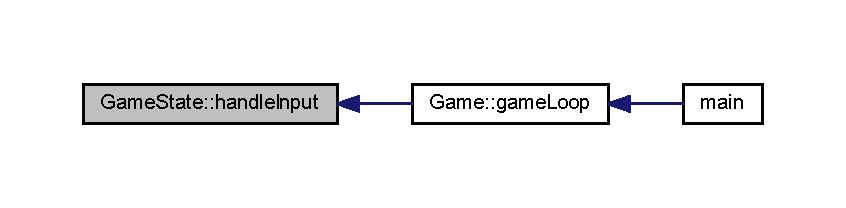
\includegraphics[width=350pt]{class_game_state_a970b55edd5a1da31ea0f7113e2c1f85a_icgraph}
\end{center}
\end{figure}


\hypertarget{class_game_state_a98cd49f1d8fd9fc3e79d607a238ba518}{\index{Game\+State@{Game\+State}!run\+Threads@{run\+Threads}}
\index{run\+Threads@{run\+Threads}!Game\+State@{Game\+State}}
\subsubsection[{run\+Threads}]{\setlength{\rightskip}{0pt plus 5cm}virtual void Game\+State\+::run\+Threads (
\begin{DoxyParamCaption}
{}
\end{DoxyParamCaption}
)\hspace{0.3cm}{\ttfamily [pure virtual]}}}\label{class_game_state_a98cd49f1d8fd9fc3e79d607a238ba518}


Implemented in \hyperlink{class_game_state_map_editor_a82ca3024c962b254ebdedcaa6ce5c1a8}{Game\+State\+Map\+Editor}, \hyperlink{class_game_state_main_menu_a2ba60c5da8bcb0c20988165a69f238a9}{Game\+State\+Main\+Menu}, \hyperlink{class_game_state_game_over_a7a9b37edd4132ee9b500a05aecfe57fb}{Game\+State\+Game\+Over}, \hyperlink{class_game_state_start_ac9514695cbd6366c721e9057aca970fe}{Game\+State\+Start}, \hyperlink{class_game_state_win_a83539ca4b809a5635d30500fa5813d1e}{Game\+State\+Win}, and \hyperlink{class_game_state_play_ab41594c10b04429a3126d4a8085de82d}{Game\+State\+Play}.

\hypertarget{class_game_state_ad331d02d3989271b8cbc88fcb1448959}{\index{Game\+State@{Game\+State}!update@{update}}
\index{update@{update}!Game\+State@{Game\+State}}
\subsubsection[{update}]{\setlength{\rightskip}{0pt plus 5cm}virtual void Game\+State\+::update (
\begin{DoxyParamCaption}
\item[{const float}]{delta\+\_\+time}
\end{DoxyParamCaption}
)\hspace{0.3cm}{\ttfamily [pure virtual]}}}\label{class_game_state_ad331d02d3989271b8cbc88fcb1448959}


Implemented in \hyperlink{class_game_state_play_a2faf041a447ddf86726658455560abb8}{Game\+State\+Play}, \hyperlink{class_game_state_map_editor_afc6fb92c082c138e86f295b99aad2ddf}{Game\+State\+Map\+Editor}, \hyperlink{class_game_state_main_menu_a796234ad5719f191b1e44affaa48026f}{Game\+State\+Main\+Menu}, \hyperlink{class_game_state_game_over_a11d874c60455411c70a9ebaab2db6a17}{Game\+State\+Game\+Over}, \hyperlink{class_game_state_start_a6a57f1c6f34ea789cb9ebf8935350627}{Game\+State\+Start}, and \hyperlink{class_game_state_win_ae8f665d71817f632afc55a665573ca8e}{Game\+State\+Win}.



Here is the caller graph for this function\+:
\nopagebreak
\begin{figure}[H]
\begin{center}
\leavevmode
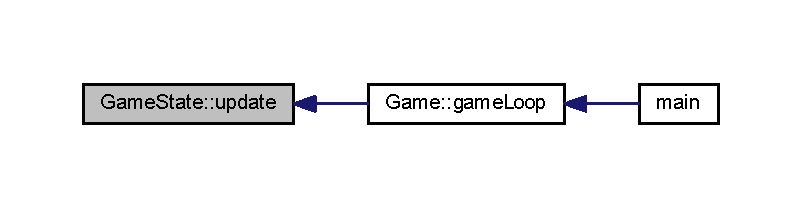
\includegraphics[width=350pt]{class_game_state_ad331d02d3989271b8cbc88fcb1448959_icgraph}
\end{center}
\end{figure}




\subsection{Member Data Documentation}
\hypertarget{class_game_state_a355a79415b9ef63c2aec1448a99f6e71}{\index{Game\+State@{Game\+State}!game@{game}}
\index{game@{game}!Game\+State@{Game\+State}}
\subsubsection[{game}]{\setlength{\rightskip}{0pt plus 5cm}{\bf Game}$\ast$ Game\+State\+::game}}\label{class_game_state_a355a79415b9ef63c2aec1448a99f6e71}


Pointer to \hyperlink{class_game}{Game} instance that handles the changing. of the states and store the info in every game state. 



The documentation for this class was generated from the following file\+:\begin{DoxyCompactItemize}
\item 
jamms/\+Tower\+Defense/\+Tower\+Defense/include/game\+States/\hyperlink{_game_state_8h}{Game\+State.\+h}\end{DoxyCompactItemize}

\hypertarget{class_game_state_main_menu}{\section{Game\+State\+Main\+Menu Class Reference}
\label{class_game_state_main_menu}\index{Game\+State\+Main\+Menu@{Game\+State\+Main\+Menu}}
}


\hyperlink{class_game}{Game} state that represents the game start, including the main game menu.  




{\ttfamily \#include $<$Game\+State\+Main\+Menu.\+h$>$}



Inheritance diagram for Game\+State\+Main\+Menu\+:\nopagebreak
\begin{figure}[H]
\begin{center}
\leavevmode
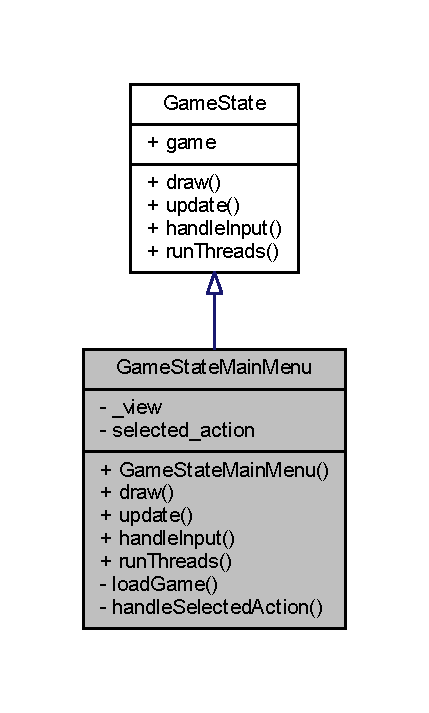
\includegraphics[width=206pt]{class_game_state_main_menu__inherit__graph}
\end{center}
\end{figure}


Collaboration diagram for Game\+State\+Main\+Menu\+:\nopagebreak
\begin{figure}[H]
\begin{center}
\leavevmode
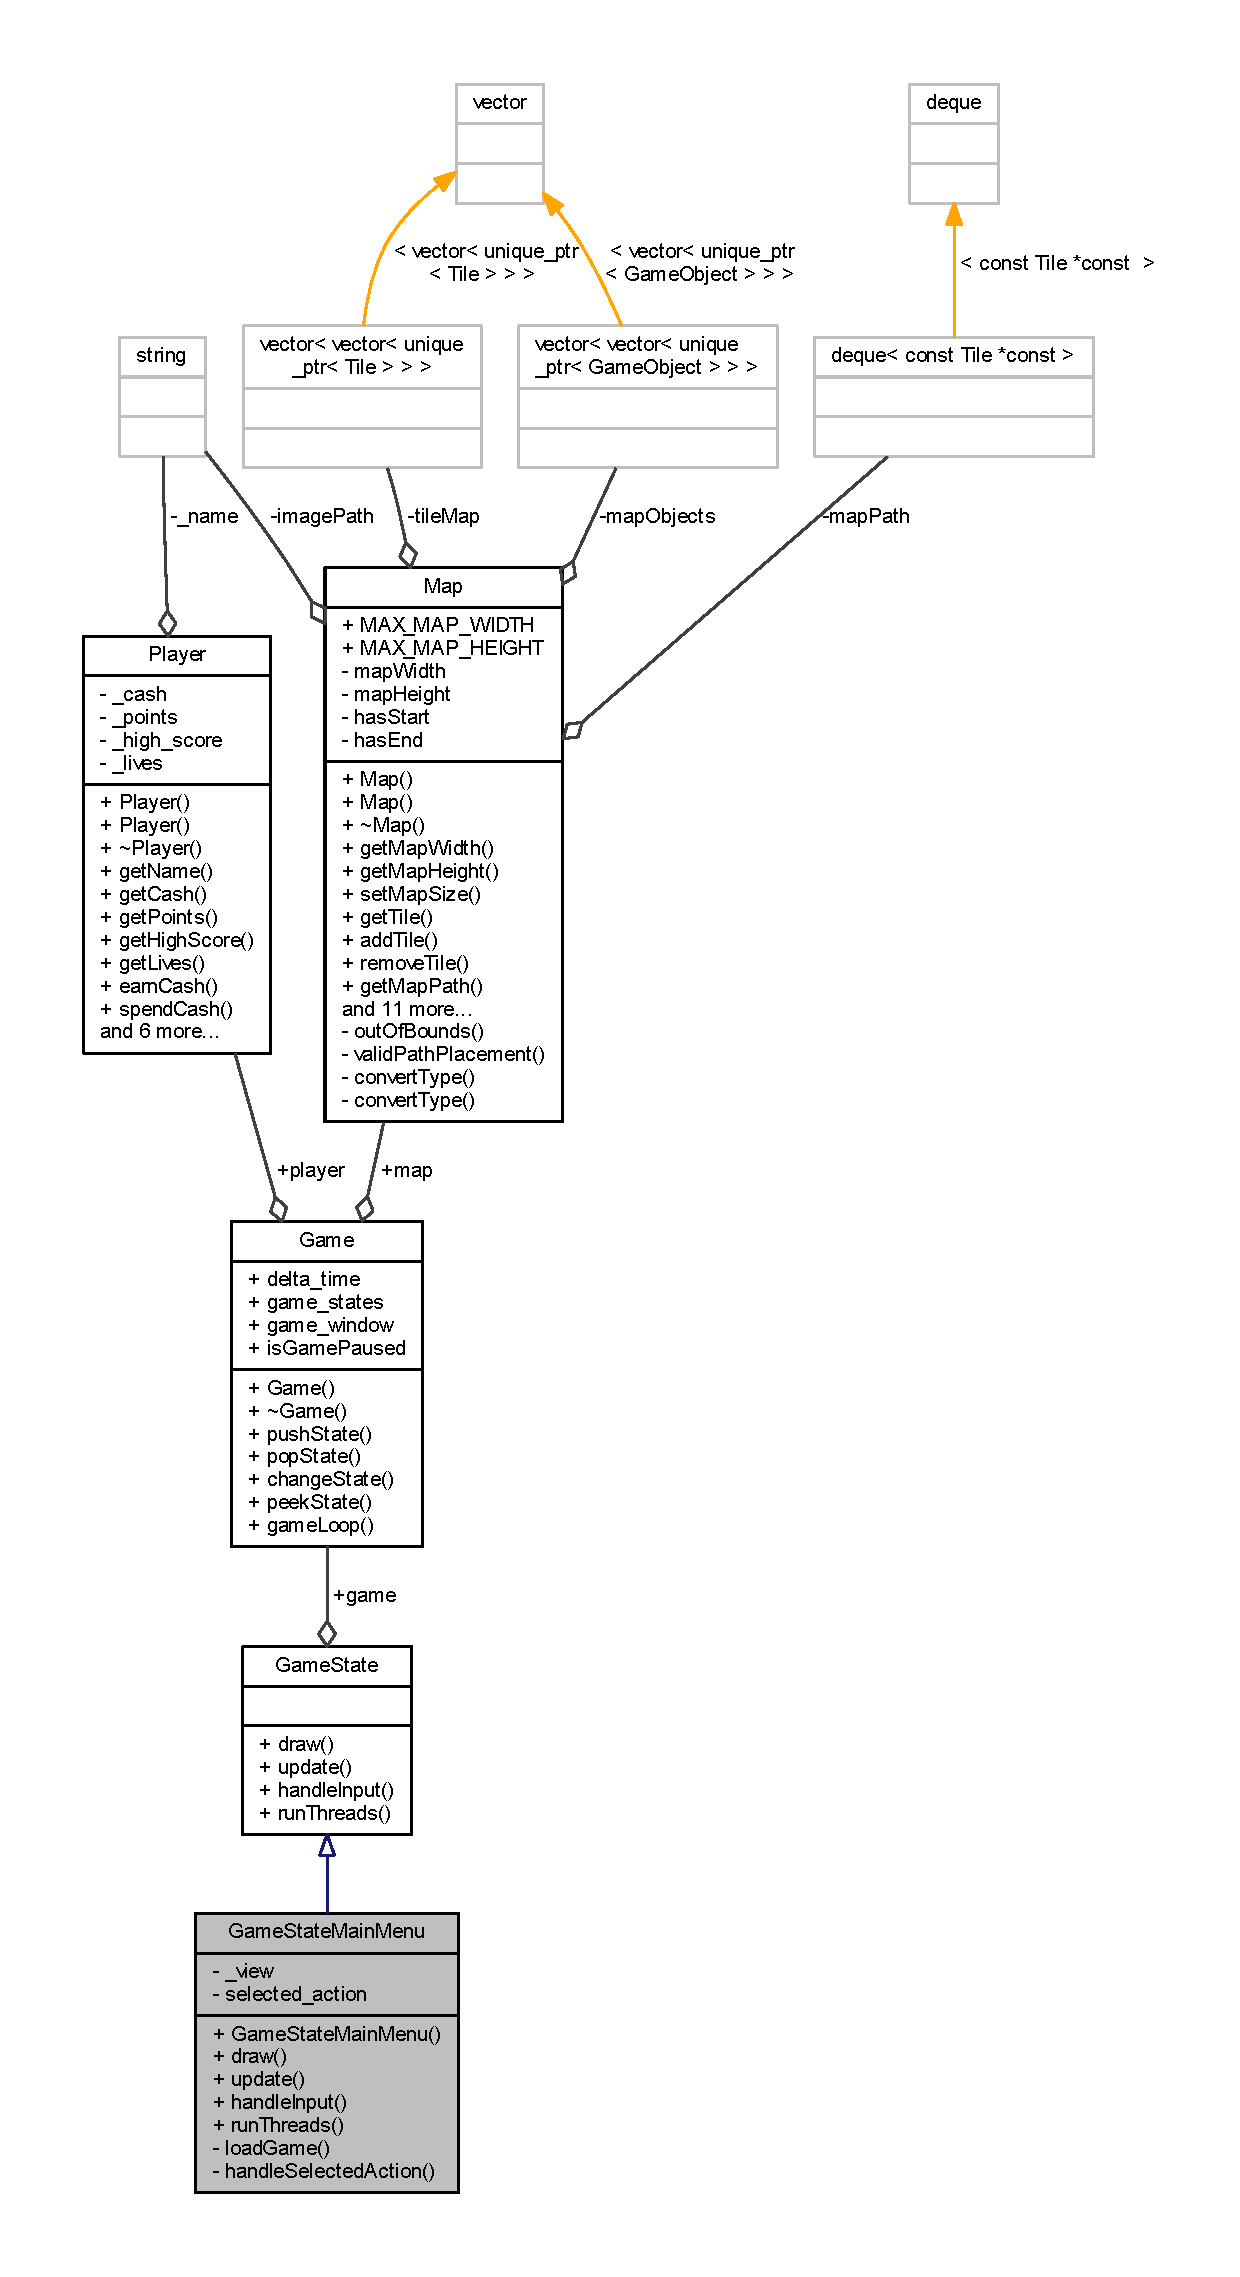
\includegraphics[height=550pt]{class_game_state_main_menu__coll__graph}
\end{center}
\end{figure}
\subsection*{Public Member Functions}
\begin{DoxyCompactItemize}
\item 
\hyperlink{class_game_state_main_menu_a7d7b3f28e70701ec9af22098b4220ec1}{Game\+State\+Main\+Menu} (\hyperlink{class_game}{Game} $\ast$\hyperlink{class_game_state_a355a79415b9ef63c2aec1448a99f6e71}{game})
\begin{DoxyCompactList}\small\item\em Constructor that takes in a pointer to the \hyperlink{class_game}{Game} that created them. \end{DoxyCompactList}\item 
virtual void \hyperlink{class_game_state_main_menu_ad34efc1ade7193ce765d00ac60f019ed}{draw} (const float delta\+\_\+time)
\begin{DoxyCompactList}\small\item\em Draws game to the render window. \end{DoxyCompactList}\item 
virtual void \hyperlink{class_game_state_main_menu_a796234ad5719f191b1e44affaa48026f}{update} (const float delta\+\_\+time)
\begin{DoxyCompactList}\small\item\em Updates game changes. \end{DoxyCompactList}\item 
virtual void \hyperlink{class_game_state_main_menu_a91ca3c60e107d135ab67c5f9e05e8aa6}{handle\+Input} ()
\begin{DoxyCompactList}\small\item\em Handles player input. \end{DoxyCompactList}\item 
virtual void \hyperlink{class_game_state_main_menu_a2ba60c5da8bcb0c20988165a69f238a9}{run\+Threads} ()
\end{DoxyCompactItemize}
\subsection*{Private Member Functions}
\begin{DoxyCompactItemize}
\item 
void \hyperlink{class_game_state_main_menu_a76d18652314696ffa6369713ef5be3ed}{load\+Game} ()
\begin{DoxyCompactList}\small\item\em Function that transitions to the \hyperlink{class_game_state_play}{Game\+State\+Play} state. \end{DoxyCompactList}\item 
void \hyperlink{class_game_state_main_menu_a85d646b336e1bb6372d851f4f654e6f1}{handle\+Selected\+Action} ()
\begin{DoxyCompactList}\small\item\em Perform the correct action given the user's selection. \end{DoxyCompactList}\end{DoxyCompactItemize}
\subsection*{Private Attributes}
\begin{DoxyCompactItemize}
\item 
sf\+::\+View \hyperlink{class_game_state_main_menu_a0c21a143cf8c10490b03da6657a81232}{\+\_\+view}
\begin{DoxyCompactList}\small\item\em Camera view for the \hyperlink{class_game_state}{Game\+State} displayed to the window. \end{DoxyCompactList}\item 
\hyperlink{class_menu_a2d708ce8df47ab5feaea1ba559a938d3}{Menu\+::\+Menu\+Action} \hyperlink{class_game_state_main_menu_ae63addaca64e4099cd1afff642e0307d}{selected\+\_\+action}
\begin{DoxyCompactList}\small\item\em The user selected action on the menu. \end{DoxyCompactList}\end{DoxyCompactItemize}
\subsection*{Additional Inherited Members}


\subsection{Detailed Description}
\hyperlink{class_game}{Game} state that represents the game start, including the main game menu. 

\subsection{Constructor \& Destructor Documentation}
\hypertarget{class_game_state_main_menu_a7d7b3f28e70701ec9af22098b4220ec1}{\index{Game\+State\+Main\+Menu@{Game\+State\+Main\+Menu}!Game\+State\+Main\+Menu@{Game\+State\+Main\+Menu}}
\index{Game\+State\+Main\+Menu@{Game\+State\+Main\+Menu}!Game\+State\+Main\+Menu@{Game\+State\+Main\+Menu}}
\subsubsection[{Game\+State\+Main\+Menu}]{\setlength{\rightskip}{0pt plus 5cm}Game\+State\+Main\+Menu\+::\+Game\+State\+Main\+Menu (
\begin{DoxyParamCaption}
\item[{{\bf Game} $\ast$}]{game}
\end{DoxyParamCaption}
)}}\label{class_game_state_main_menu_a7d7b3f28e70701ec9af22098b4220ec1}


Constructor that takes in a pointer to the \hyperlink{class_game}{Game} that created them. 


\begin{DoxyParams}{Parameters}
{\em game} & Pointer to game.\\
\hline
\end{DoxyParams}
The constructor sets the view to the size of the window and centers the view on the center of the window. 

\subsection{Member Function Documentation}
\hypertarget{class_game_state_main_menu_ad34efc1ade7193ce765d00ac60f019ed}{\index{Game\+State\+Main\+Menu@{Game\+State\+Main\+Menu}!draw@{draw}}
\index{draw@{draw}!Game\+State\+Main\+Menu@{Game\+State\+Main\+Menu}}
\subsubsection[{draw}]{\setlength{\rightskip}{0pt plus 5cm}void Game\+State\+Main\+Menu\+::draw (
\begin{DoxyParamCaption}
\item[{const float}]{delta\+\_\+time}
\end{DoxyParamCaption}
)\hspace{0.3cm}{\ttfamily [virtual]}}}\label{class_game_state_main_menu_ad34efc1ade7193ce765d00ac60f019ed}


Draws game to the render window. 


\begin{DoxyParams}{Parameters}
{\em delta\+\_\+time} & Elapsed time during the game. \\
\hline
\end{DoxyParams}
\begin{DoxyReturn}{Returns}
Void.
\end{DoxyReturn}
This function sets the view to be drawn to the window and also calls a function to draw the splash screen. 

Implements \hyperlink{class_game_state_a55a6a68aabdf7054ea0e6ddbf24902df}{Game\+State}.



Here is the call graph for this function\+:\nopagebreak
\begin{figure}[H]
\begin{center}
\leavevmode
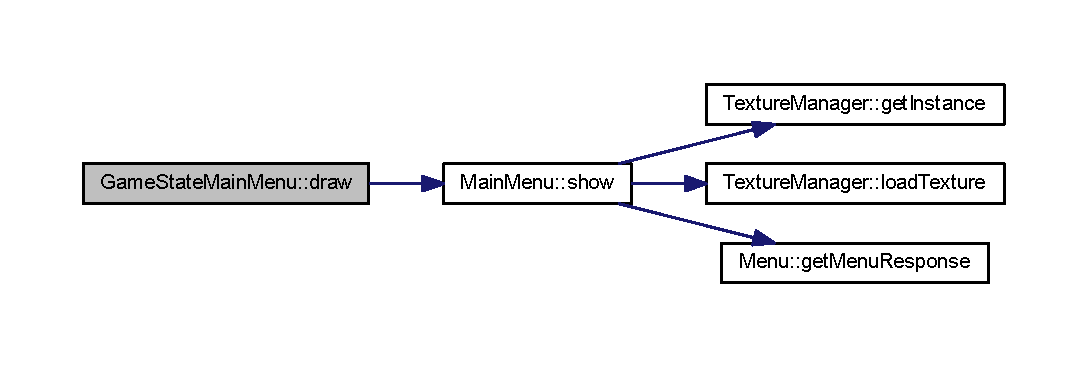
\includegraphics[width=350pt]{class_game_state_main_menu_ad34efc1ade7193ce765d00ac60f019ed_cgraph}
\end{center}
\end{figure}


\hypertarget{class_game_state_main_menu_a91ca3c60e107d135ab67c5f9e05e8aa6}{\index{Game\+State\+Main\+Menu@{Game\+State\+Main\+Menu}!handle\+Input@{handle\+Input}}
\index{handle\+Input@{handle\+Input}!Game\+State\+Main\+Menu@{Game\+State\+Main\+Menu}}
\subsubsection[{handle\+Input}]{\setlength{\rightskip}{0pt plus 5cm}void Game\+State\+Main\+Menu\+::handle\+Input (
\begin{DoxyParamCaption}
{}
\end{DoxyParamCaption}
)\hspace{0.3cm}{\ttfamily [virtual]}}}\label{class_game_state_main_menu_a91ca3c60e107d135ab67c5f9e05e8aa6}


Handles player input. 

\begin{DoxyReturn}{Returns}
Void. 
\end{DoxyReturn}


Implements \hyperlink{class_game_state_a970b55edd5a1da31ea0f7113e2c1f85a}{Game\+State}.



Here is the call graph for this function\+:\nopagebreak
\begin{figure}[H]
\begin{center}
\leavevmode
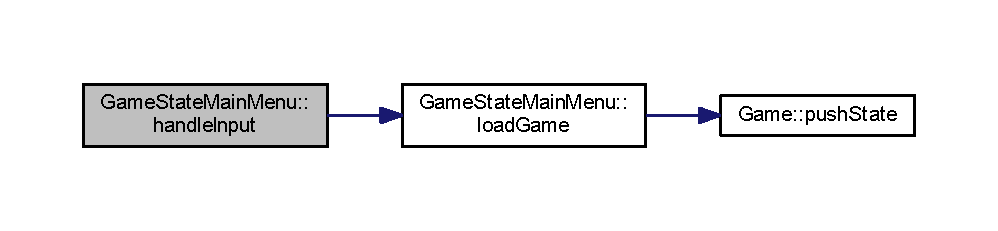
\includegraphics[width=350pt]{class_game_state_main_menu_a91ca3c60e107d135ab67c5f9e05e8aa6_cgraph}
\end{center}
\end{figure}


\hypertarget{class_game_state_main_menu_a85d646b336e1bb6372d851f4f654e6f1}{\index{Game\+State\+Main\+Menu@{Game\+State\+Main\+Menu}!handle\+Selected\+Action@{handle\+Selected\+Action}}
\index{handle\+Selected\+Action@{handle\+Selected\+Action}!Game\+State\+Main\+Menu@{Game\+State\+Main\+Menu}}
\subsubsection[{handle\+Selected\+Action}]{\setlength{\rightskip}{0pt plus 5cm}void Game\+State\+Main\+Menu\+::handle\+Selected\+Action (
\begin{DoxyParamCaption}
{}
\end{DoxyParamCaption}
)\hspace{0.3cm}{\ttfamily [private]}}}\label{class_game_state_main_menu_a85d646b336e1bb6372d851f4f654e6f1}


Perform the correct action given the user's selection. 

\begin{DoxyReturn}{Returns}
Void. 
\end{DoxyReturn}
\hypertarget{class_game_state_main_menu_a76d18652314696ffa6369713ef5be3ed}{\index{Game\+State\+Main\+Menu@{Game\+State\+Main\+Menu}!load\+Game@{load\+Game}}
\index{load\+Game@{load\+Game}!Game\+State\+Main\+Menu@{Game\+State\+Main\+Menu}}
\subsubsection[{load\+Game}]{\setlength{\rightskip}{0pt plus 5cm}void Game\+State\+Main\+Menu\+::load\+Game (
\begin{DoxyParamCaption}
{}
\end{DoxyParamCaption}
)\hspace{0.3cm}{\ttfamily [private]}}}\label{class_game_state_main_menu_a76d18652314696ffa6369713ef5be3ed}


Function that transitions to the \hyperlink{class_game_state_play}{Game\+State\+Play} state. 

\begin{DoxyReturn}{Returns}
Void.
\end{DoxyReturn}
Add the \hyperlink{class_game_state_play}{Game\+State\+Play} state to the game 

Here is the call graph for this function\+:\nopagebreak
\begin{figure}[H]
\begin{center}
\leavevmode
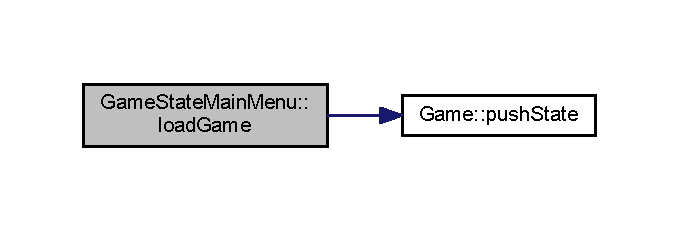
\includegraphics[width=326pt]{class_game_state_main_menu_a76d18652314696ffa6369713ef5be3ed_cgraph}
\end{center}
\end{figure}




Here is the caller graph for this function\+:\nopagebreak
\begin{figure}[H]
\begin{center}
\leavevmode
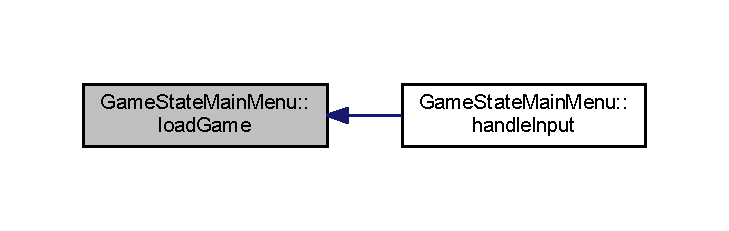
\includegraphics[width=350pt]{class_game_state_main_menu_a76d18652314696ffa6369713ef5be3ed_icgraph}
\end{center}
\end{figure}


\hypertarget{class_game_state_main_menu_a2ba60c5da8bcb0c20988165a69f238a9}{\index{Game\+State\+Main\+Menu@{Game\+State\+Main\+Menu}!run\+Threads@{run\+Threads}}
\index{run\+Threads@{run\+Threads}!Game\+State\+Main\+Menu@{Game\+State\+Main\+Menu}}
\subsubsection[{run\+Threads}]{\setlength{\rightskip}{0pt plus 5cm}virtual void Game\+State\+Main\+Menu\+::run\+Threads (
\begin{DoxyParamCaption}
{}
\end{DoxyParamCaption}
)\hspace{0.3cm}{\ttfamily [inline]}, {\ttfamily [virtual]}}}\label{class_game_state_main_menu_a2ba60c5da8bcb0c20988165a69f238a9}


Implements \hyperlink{class_game_state_a98cd49f1d8fd9fc3e79d607a238ba518}{Game\+State}.

\hypertarget{class_game_state_main_menu_a796234ad5719f191b1e44affaa48026f}{\index{Game\+State\+Main\+Menu@{Game\+State\+Main\+Menu}!update@{update}}
\index{update@{update}!Game\+State\+Main\+Menu@{Game\+State\+Main\+Menu}}
\subsubsection[{update}]{\setlength{\rightskip}{0pt plus 5cm}virtual void Game\+State\+Main\+Menu\+::update (
\begin{DoxyParamCaption}
\item[{const float}]{delta\+\_\+time}
\end{DoxyParamCaption}
)\hspace{0.3cm}{\ttfamily [inline]}, {\ttfamily [virtual]}}}\label{class_game_state_main_menu_a796234ad5719f191b1e44affaa48026f}


Updates game changes. 


\begin{DoxyParams}{Parameters}
{\em delta\+\_\+time} & Elapsed time during the game. \\
\hline
\end{DoxyParams}
\begin{DoxyReturn}{Returns}
Void. 
\end{DoxyReturn}


Implements \hyperlink{class_game_state_ad331d02d3989271b8cbc88fcb1448959}{Game\+State}.



\subsection{Member Data Documentation}
\hypertarget{class_game_state_main_menu_a0c21a143cf8c10490b03da6657a81232}{\index{Game\+State\+Main\+Menu@{Game\+State\+Main\+Menu}!\+\_\+view@{\+\_\+view}}
\index{\+\_\+view@{\+\_\+view}!Game\+State\+Main\+Menu@{Game\+State\+Main\+Menu}}
\subsubsection[{\+\_\+view}]{\setlength{\rightskip}{0pt plus 5cm}sf\+::\+View Game\+State\+Main\+Menu\+::\+\_\+view\hspace{0.3cm}{\ttfamily [private]}}}\label{class_game_state_main_menu_a0c21a143cf8c10490b03da6657a81232}


Camera view for the \hyperlink{class_game_state}{Game\+State} displayed to the window. 

\hypertarget{class_game_state_main_menu_ae63addaca64e4099cd1afff642e0307d}{\index{Game\+State\+Main\+Menu@{Game\+State\+Main\+Menu}!selected\+\_\+action@{selected\+\_\+action}}
\index{selected\+\_\+action@{selected\+\_\+action}!Game\+State\+Main\+Menu@{Game\+State\+Main\+Menu}}
\subsubsection[{selected\+\_\+action}]{\setlength{\rightskip}{0pt plus 5cm}{\bf Menu\+::\+Menu\+Action} Game\+State\+Main\+Menu\+::selected\+\_\+action\hspace{0.3cm}{\ttfamily [private]}}}\label{class_game_state_main_menu_ae63addaca64e4099cd1afff642e0307d}


The user selected action on the menu. 



The documentation for this class was generated from the following files\+:\begin{DoxyCompactItemize}
\item 
jamms/\+Tower\+Defense/\+Tower\+Defense/include/game\+States/\hyperlink{_game_state_main_menu_8h}{Game\+State\+Main\+Menu.\+h}\item 
jamms/\+Tower\+Defense/\+Tower\+Defense/src/game\+States/\hyperlink{_game_state_main_menu_8cpp}{Game\+State\+Main\+Menu.\+cpp}\end{DoxyCompactItemize}

\hypertarget{class_game_state_play}{\section{Game\+State\+Play Class Reference}
\label{class_game_state_play}\index{Game\+State\+Play@{Game\+State\+Play}}
}


\hyperlink{class_game}{Game} state that represents the gameplay.  




{\ttfamily \#include $<$Game\+State\+Play.\+h$>$}



Inheritance diagram for Game\+State\+Play\+:
\nopagebreak
\begin{figure}[H]
\begin{center}
\leavevmode
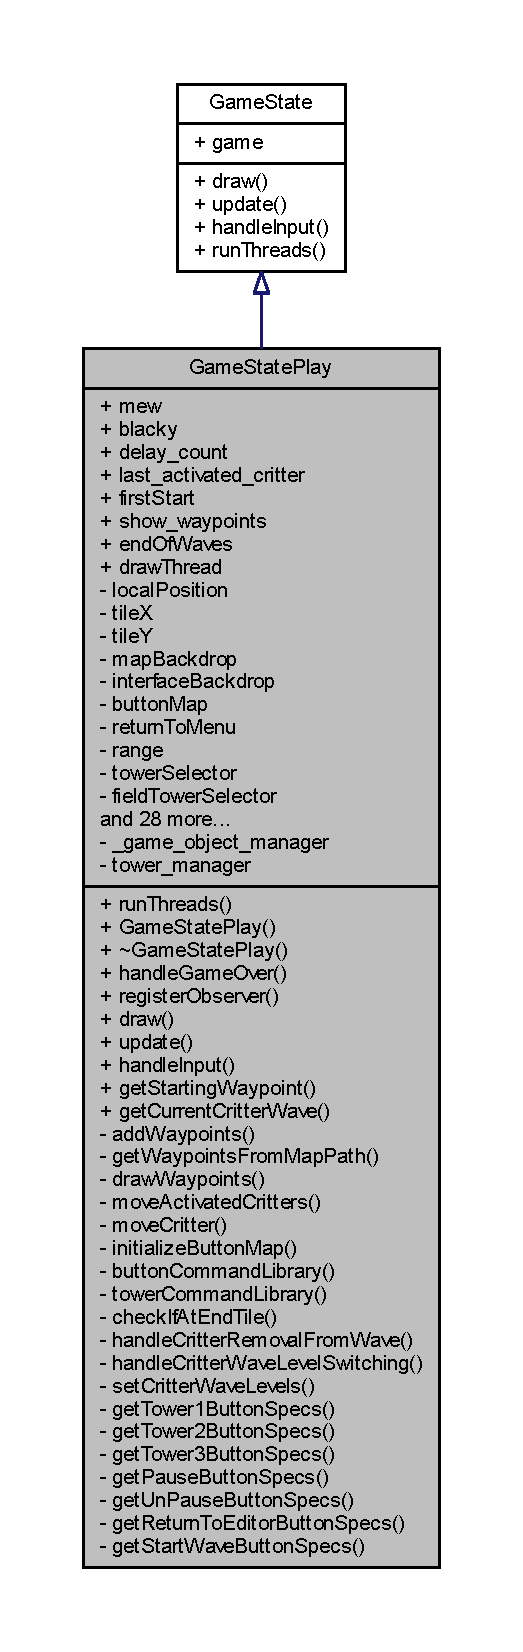
\includegraphics[height=550pt]{class_game_state_play__inherit__graph}
\end{center}
\end{figure}


Collaboration diagram for Game\+State\+Play\+:
\nopagebreak
\begin{figure}[H]
\begin{center}
\leavevmode
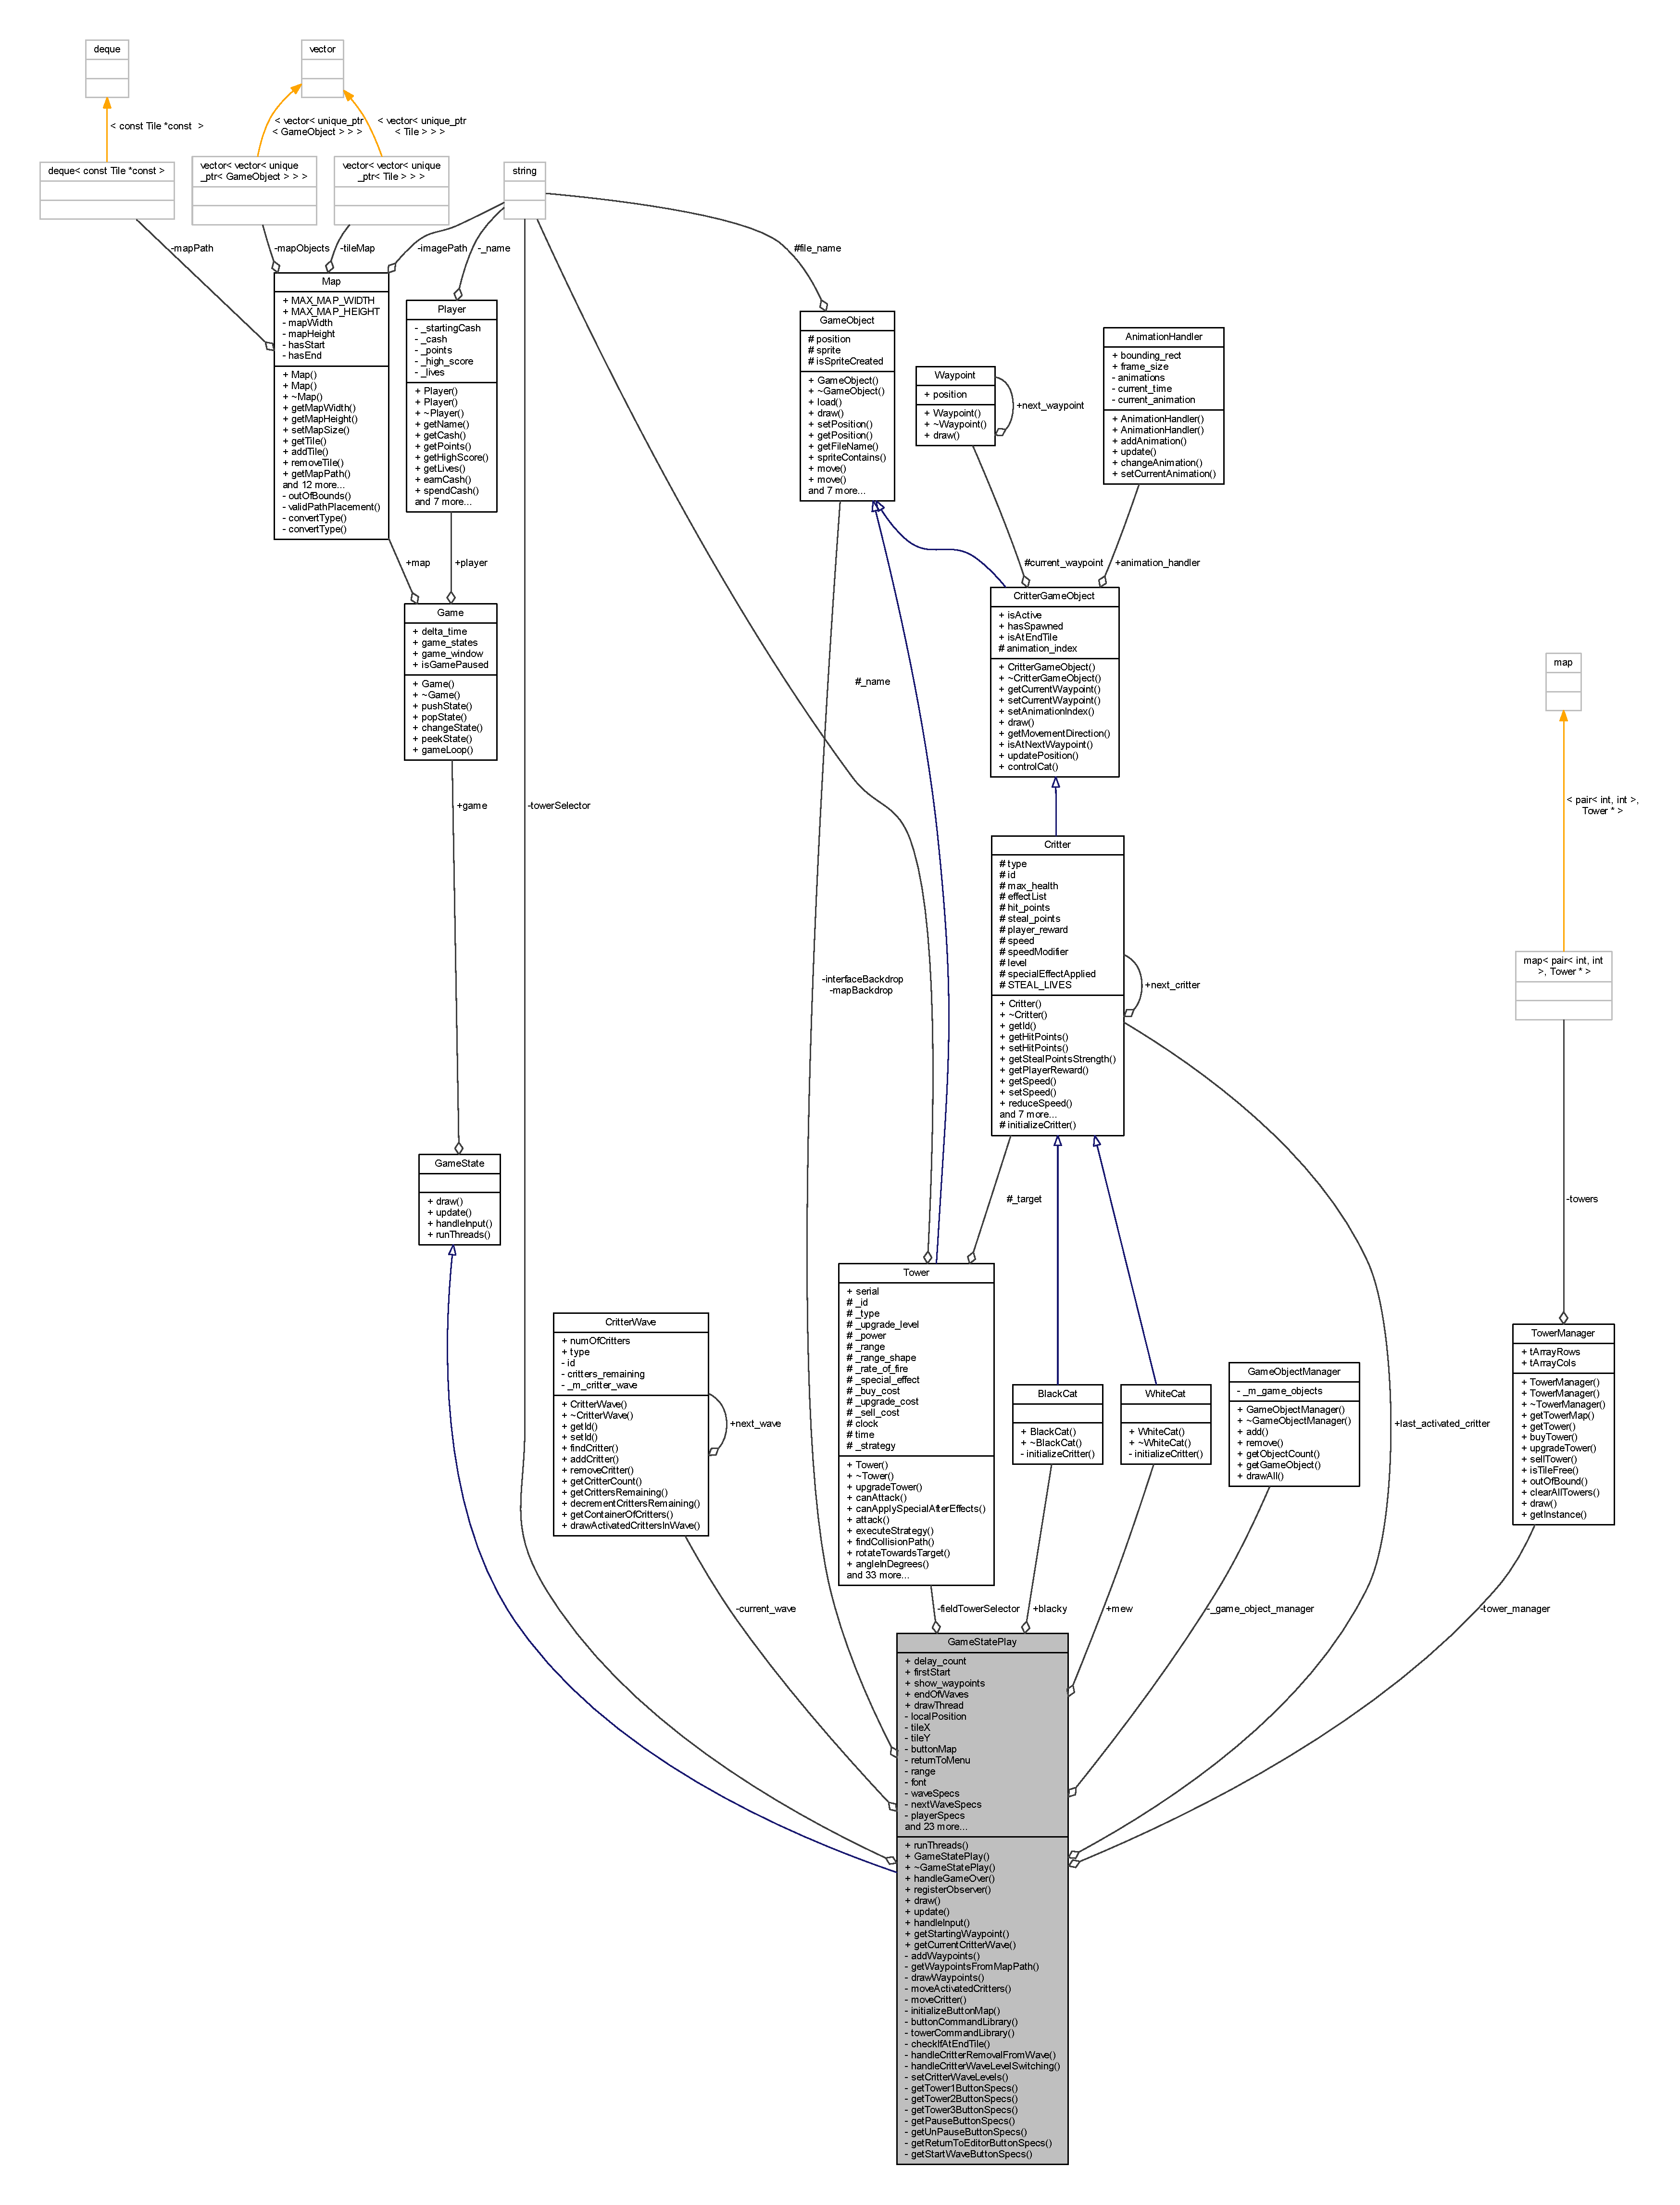
\includegraphics[width=350pt]{class_game_state_play__coll__graph}
\end{center}
\end{figure}
\subsection*{Public Member Functions}
\begin{DoxyCompactItemize}
\item 
virtual void \hyperlink{class_game_state_play_ab41594c10b04429a3126d4a8085de82d}{run\+Threads} ()
\item 
\hyperlink{class_game_state_play_a705c09eac3d2b27757e5b4cc048b22d5}{Game\+State\+Play} (\hyperlink{class_game}{Game} $\ast$\hyperlink{class_game_state_a355a79415b9ef63c2aec1448a99f6e71}{game})
\begin{DoxyCompactList}\small\item\em Constructor that takes in a pointer to the \hyperlink{class_game}{Game} that created them. \end{DoxyCompactList}\item 
\hyperlink{class_game_state_play_ae4f10dc83f16da01f425d09f9fbb4ef6}{$\sim$\+Game\+State\+Play} ()
\item 
void \hyperlink{class_game_state_play_aec5f72cea0e80d1d83b9cbe155a65ce9}{handle\+Game\+Over} ()
\item 
void \hyperlink{class_game_state_play_a5076f9d4d81b1b9dc4e71c627f40a9d2}{register\+Observer} (\hyperlink{class_tower}{Tower} $\ast$tower)
\item 
virtual void \hyperlink{class_game_state_play_a63a3ba0c891afd8ec126806bab4f315a}{draw} (const float delta\+\_\+time)
\begin{DoxyCompactList}\small\item\em Draws game to the render window. \end{DoxyCompactList}\item 
virtual void \hyperlink{class_game_state_play_a2faf041a447ddf86726658455560abb8}{update} (const float delta\+\_\+time)
\begin{DoxyCompactList}\small\item\em Updates game changes. \end{DoxyCompactList}\item 
virtual void \hyperlink{class_game_state_play_ae9acc781e1fdbc931784ba3892c469ce}{handle\+Input} ()
\begin{DoxyCompactList}\small\item\em Handles player input. \end{DoxyCompactList}\item 
\hyperlink{class_waypoint}{Waypoint} $\ast$ \hyperlink{class_game_state_play_a6ebd21112217871afe2e0160f6eb0753}{get\+Starting\+Waypoint} ()
\begin{DoxyCompactList}\small\item\em Get starting waypoint. \end{DoxyCompactList}\item 
\hyperlink{class_critter_wave}{Critter\+Wave} $\ast$ \hyperlink{class_game_state_play_a36f7d1ee2a500290e224a50f679ba3ff}{get\+Current\+Critter\+Wave} ()
\end{DoxyCompactItemize}
\subsection*{Public Attributes}
\begin{DoxyCompactItemize}
\item 
\hyperlink{class_white_cat}{White\+Cat} $\ast$ \hyperlink{class_game_state_play_a90934640484bd6417007e112d8034a50}{mew}
\item 
\hyperlink{class_black_cat}{Black\+Cat} $\ast$ \hyperlink{class_game_state_play_ace195ef46750d243d3bbaf2abaaf6e2e}{blacky}
\item 
int \hyperlink{class_game_state_play_aa0948c192d3ef1adb6eaaeade8521733}{delay\+\_\+count}
\item 
\hyperlink{class_critter}{Critter} $\ast$ \hyperlink{class_game_state_play_ad6c5af538edc9f5b2fd3ba0c0f95e89d}{last\+\_\+activated\+\_\+critter}
\item 
bool \hyperlink{class_game_state_play_a59cc893637827eb0d9ee902262548980}{first\+Start}
\item 
bool \hyperlink{class_game_state_play_a406124f1525e8555fb264c743298d7b9}{show\+\_\+waypoints}
\item 
bool \hyperlink{class_game_state_play_a0e613be489b2c61857676303a15ce3cc}{end\+Of\+Waves}
\item 
std\+::thread \hyperlink{class_game_state_play_aac5b1d9de4ab0ad2445d97a588cb3168}{draw\+Thread}
\end{DoxyCompactItemize}
\subsection*{Private Member Functions}
\begin{DoxyCompactItemize}
\item 
std\+::vector$<$ \hyperlink{class_waypoint}{Waypoint} $>$ \hyperlink{class_game_state_play_aee1a80f02dd69d8f06c041020eb4447e}{add\+Waypoints} (std\+::vector$<$ sf\+::\+Vector2f $>$ path\+\_\+points)
\begin{DoxyCompactList}\small\item\em Add waypoints. \end{DoxyCompactList}\item 
std\+::vector$<$ sf\+::\+Vector2f $>$ \hyperlink{class_game_state_play_aae84ae33a68caa8bf05a4a2a49a2b41d}{get\+Waypoints\+From\+Map\+Path} ()
\begin{DoxyCompactList}\small\item\em Create waypoint vector from the map's path. \end{DoxyCompactList}\item 
void \hyperlink{class_game_state_play_a28fee46c0b9d0248ed319976be94494a}{draw\+Waypoints} (std\+::vector$<$ \hyperlink{class_waypoint}{Waypoint} $>$ waypoints, sf\+::\+Render\+Window \&game\+\_\+window)
\begin{DoxyCompactList}\small\item\em Draw all waypoints. \end{DoxyCompactList}\item 
void \hyperlink{class_game_state_play_ae812a7447027abe5fcc2f79bf3e35ad8}{move\+Activated\+Critters} (const float delta\+\_\+time)
\item 
void \hyperlink{class_game_state_play_a0d6ff2e65992c5fb29f180c6b1eb9435}{move\+Critter} (\hyperlink{class_critter}{Critter} $\ast$critter, const float delta\+\_\+time)
\item 
void \hyperlink{class_game_state_play_a3a6947bfe8be3d1974094acb8362eda9}{initialize\+Button\+Map} ()
\item 
void \hyperlink{class_game_state_play_a79237473ceeb26b94f641d0bf66c1ec0}{button\+Command\+Library} ()
\item 
void \hyperlink{class_game_state_play_ab33de76aa28534d14aa1d79bed43aa17}{tower\+Command\+Library} (const int \hyperlink{class_game_state_play_a6c82bd77433f30b20a88e19ab37a7f96}{tile\+X}, const int \hyperlink{class_game_state_play_ae34c6aa315832bd457df59720345534e}{tile\+Y})
\item 
bool \hyperlink{class_game_state_play_ac82134049ed6dd0aaa929e200f7185d5}{check\+If\+At\+End\+Tile} (\hyperlink{class_critter}{Critter} $\ast$critter)
\item 
void \hyperlink{class_game_state_play_a2278751d53b50beb97c809db26f1b9b6}{handle\+Critter\+Removal\+From\+Wave} ()
\item 
void \hyperlink{class_game_state_play_a2eda31c4d98a8440c6eba38604aa2a79}{handle\+Critter\+Wave\+Level\+Switching} ()
\item 
void \hyperlink{class_game_state_play_a6047cbdce7daa2092d95bf786db5267a}{set\+Critter\+Wave\+Levels} (\hyperlink{class_waypoint}{Waypoint} $\ast$starting\+\_\+waypoint)
\end{DoxyCompactItemize}
\subsection*{Static Private Member Functions}
\begin{DoxyCompactItemize}
\item 
static std\+::string \hyperlink{class_game_state_play_a11c1d1976d85631c84a8db18b1458637}{get\+Tower1\+Button\+Specs} ()
\item 
static std\+::string \hyperlink{class_game_state_play_a0b9e886dc6a80b52f559441c7a3455d8}{get\+Tower2\+Button\+Specs} ()
\item 
static std\+::string \hyperlink{class_game_state_play_a0c79cb57b169ec8c0dc08c49451ebfc1}{get\+Tower3\+Button\+Specs} ()
\item 
static std\+::string \hyperlink{class_game_state_play_a84292b8af5919f8da3b54c1d1dba5cfd}{get\+Pause\+Button\+Specs} ()
\item 
static std\+::string \hyperlink{class_game_state_play_a93771d14333ebc475f2428d3c1a3c3d3}{get\+Un\+Pause\+Button\+Specs} ()
\item 
static std\+::string \hyperlink{class_game_state_play_aed4df6e7af126ba32ac06eb5dd79694d}{get\+Return\+To\+Editor\+Button\+Specs} ()
\item 
static std\+::string \hyperlink{class_game_state_play_ace72b0eb76edd4a7e02ab12454f9f5b7}{get\+Start\+Wave\+Button\+Specs} ()
\end{DoxyCompactItemize}
\subsection*{Private Attributes}
\begin{DoxyCompactItemize}
\item 
sf\+::\+Vector2i \hyperlink{class_game_state_play_aef4648e9978d2b031365686fa5221038}{local\+Position}
\item 
int \hyperlink{class_game_state_play_a6c82bd77433f30b20a88e19ab37a7f96}{tile\+X}
\item 
int \hyperlink{class_game_state_play_ae34c6aa315832bd457df59720345534e}{tile\+Y}
\item 
\hyperlink{class_game_object}{Game\+Object} \hyperlink{class_game_state_play_a1114fc8f3e15f5f46ab4361dad37ad0b}{map\+Backdrop}
\item 
\hyperlink{class_game_object}{Game\+Object} \hyperlink{class_game_state_play_a153cd0b94e19f3c0fab378c716678f60}{interface\+Backdrop}
\item 
std\+::map$<$ string, \hyperlink{class_game_object}{Game\+Object} $>$ \hyperlink{class_game_state_play_ab0755d9a7eb5708a840d82bbdc7eb9f2}{button\+Map}
\item 
bool \hyperlink{class_game_state_play_a6f5a18b6d0597c0f6c4d26b4df873ee6}{return\+To\+Menu}
\item 
sf\+::\+Circle\+Shape \hyperlink{class_game_state_play_a4ac9c1b314dfbfe0082728eacfc401fc}{range}
\item 
std\+::string \hyperlink{class_game_state_play_acfd6271509da5b9cec7ed2904b3ad33a}{tower\+Selector}
\item 
\hyperlink{class_tower}{Tower} $\ast$ \hyperlink{class_game_state_play_af37399cc10da66842740622a891489e0}{field\+Tower\+Selector}
\item 
sf\+::\+Font \hyperlink{class_game_state_play_a333494e6c4a8ae4a285635776c3b486e}{font}
\item 
sf\+::\+Text \hyperlink{class_game_state_play_a61669dc94331d0302f3a0f5792304049}{wave\+Specs}
\item 
sf\+::\+Text \hyperlink{class_game_state_play_afee193abc64a41d61a08db7d6d5b507d}{next\+Wave\+Specs}
\item 
sf\+::\+Text \hyperlink{class_game_state_play_a5e7f3929ab226b4ad0fb627d3c779f84}{player\+Specs}
\item 
sf\+::\+Text \hyperlink{class_game_state_play_add98cf58c2cc6af809cade72be6c6c0a}{tower\+Specs}
\item 
sf\+::\+Text \hyperlink{class_game_state_play_a1667ea17be43ded7176a9dc28d99a8e1}{critter\+Specs}
\item 
sf\+::\+Text \hyperlink{class_game_state_play_a65d1a4d74f886ce3de872c1ffbb63d57}{button\+Specs}
\item 
sf\+::\+Text \hyperlink{class_game_state_play_ac8809caa817213fe1b78749b3b19ad6f}{selected\+Tower\+Specs}
\item 
sf\+::\+Text \hyperlink{class_game_state_play_ae1ee7931ef89e141f54ad6588759ea6f}{nearest\+Tower}
\item 
sf\+::\+Text \hyperlink{class_game_state_play_a4ca301f18fc6be19a8465721a6c3bb1f}{nearest\+End}
\item 
sf\+::\+Text \hyperlink{class_game_state_play_a19bbd6c5ddab619c2fed65c1a368395d}{strongest}
\item 
sf\+::\+Text \hyperlink{class_game_state_play_aa528568bfe4f5fcc79605557c6d0d12d}{weakest}
\item 
sf\+::\+Text \hyperlink{class_game_state_play_a1ff2a6f5c9983a5240afa2aa94c3d034}{most\+H}
\item 
sf\+::\+Text \hyperlink{class_game_state_play_a68ba25d35cbc05415be9173aac2ce4c1}{least\+H}
\item 
sf\+::\+Text \hyperlink{class_game_state_play_aa5a191ff7adb99b88d5c967f44880264}{slowest}
\item 
sf\+::\+Text \hyperlink{class_game_state_play_a6b8fba9f1816c183dc546ccbe8fc04cc}{fastest}
\item 
sf\+::\+Text \hyperlink{class_game_state_play_a2d77b920db04a5a69e86625200631dd7}{most\+Coins}
\item 
std\+::map$<$ int, sf\+::\+Text $>$ \hyperlink{class_game_state_play_a7ca10b4aceefc0e2732ec427c5b5b5c5}{critter\+Health}
\item 
std\+::map$<$ int, sf\+::\+Clock $>$ \hyperlink{class_game_state_play_af65d40be0eb5748b1d80186cefd3cc71}{health\+Clock}
\item 
sf\+::\+Time \hyperlink{class_game_state_play_a4a2fd0f59504ad64f5d8b871cbf3cd35}{health\+Time}
\item 
std\+::map$<$ int, sf\+::\+Text $>$ \hyperlink{class_game_state_play_a2c0118859e607a1ef2aa008f1b94b7f8}{effect\+Damage}
\item 
std\+::map$<$ int, sf\+::\+Clock $>$ \hyperlink{class_game_state_play_a672216db210bc2dca82196badc7c20e9}{effect\+Damage\+Clock}
\item 
sf\+::\+Time \hyperlink{class_game_state_play_a9d324dec79041681951cf84349507e7f}{effect\+Damage\+Time}
\item 
sf\+::\+View \hyperlink{class_game_state_play_a9513cfeac2178d83e23ba6f9291fba8c}{\+\_\+game\+View}
\begin{DoxyCompactList}\small\item\em Camera view for the gameplay displayed to the window. \end{DoxyCompactList}\item 
sf\+::\+View \hyperlink{class_game_state_play_affee804e287fd1968fe8c5b0a303b05d}{\+\_\+gui\+View}
\begin{DoxyCompactList}\small\item\em Camera view for the H\+U\+D displayed to the window. \end{DoxyCompactList}\item 
\hyperlink{class_critter_wave}{Critter\+Wave} $\ast$ \hyperlink{class_game_state_play_a64cd6841a6f7139ff7e3747e4159654c}{current\+\_\+wave}
\item 
std\+::vector$<$ \hyperlink{class_critter_wave}{Critter\+Wave} $\ast$ $>$ \hyperlink{class_game_state_play_a97b5c39127688b4c5ddb147572f77290}{wave\+\_\+levels}
\item 
std\+::vector$<$ \hyperlink{class_waypoint}{Waypoint} $>$ \hyperlink{class_game_state_play_a14914e609fd8b83324b3fc47343ec19a}{current\+\_\+waypoints}
\end{DoxyCompactItemize}
\subsection*{Static Private Attributes}
\begin{DoxyCompactItemize}
\item 
static \hyperlink{class_game_object_manager}{Game\+Object\+Manager} \hyperlink{class_game_state_play_a3f05ff560a8dbeb5a1922e23c6bbff72}{\+\_\+game\+\_\+object\+\_\+manager}
\item 
static \hyperlink{class_tower_manager}{Tower\+Manager} \& \hyperlink{class_game_state_play_a951af277d5a8a7fca23fe3240be847c9}{tower\+\_\+manager} = \hyperlink{class_tower_manager_ad23044e56ca84962064cfcb9bee3adaf}{Tower\+Manager\+::get\+Instance}()
\end{DoxyCompactItemize}


\subsection{Detailed Description}
\hyperlink{class_game}{Game} state that represents the gameplay. 

\subsection{Constructor \& Destructor Documentation}
\hypertarget{class_game_state_play_a705c09eac3d2b27757e5b4cc048b22d5}{\index{Game\+State\+Play@{Game\+State\+Play}!Game\+State\+Play@{Game\+State\+Play}}
\index{Game\+State\+Play@{Game\+State\+Play}!Game\+State\+Play@{Game\+State\+Play}}
\subsubsection[{Game\+State\+Play}]{\setlength{\rightskip}{0pt plus 5cm}Game\+State\+Play\+::\+Game\+State\+Play (
\begin{DoxyParamCaption}
\item[{{\bf Game} $\ast$}]{game}
\end{DoxyParamCaption}
)}}\label{class_game_state_play_a705c09eac3d2b27757e5b4cc048b22d5}


Constructor that takes in a pointer to the \hyperlink{class_game}{Game} that created them. 


\begin{DoxyParams}{Parameters}
{\em game} & Pointer to game.\\
\hline
\end{DoxyParams}
The constructor sets the view to the size of the window and centers the view on the center of the window. 

Here is the call graph for this function\+:\nopagebreak
\begin{figure}[H]
\begin{center}
\leavevmode
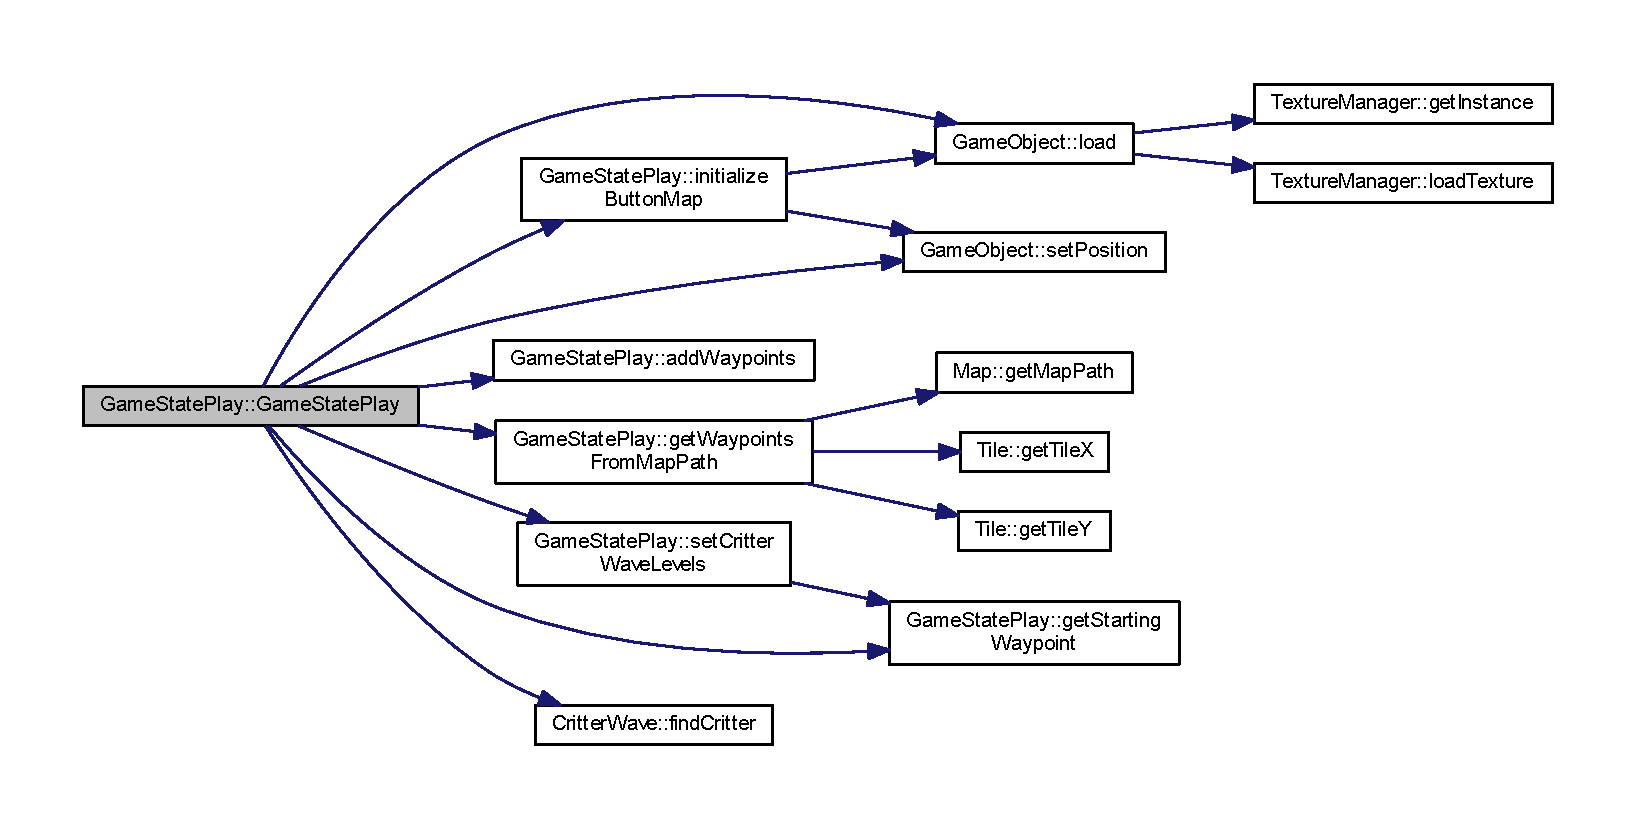
\includegraphics[width=350pt]{class_game_state_play_a705c09eac3d2b27757e5b4cc048b22d5_cgraph}
\end{center}
\end{figure}


\hypertarget{class_game_state_play_ae4f10dc83f16da01f425d09f9fbb4ef6}{\index{Game\+State\+Play@{Game\+State\+Play}!````~Game\+State\+Play@{$\sim$\+Game\+State\+Play}}
\index{````~Game\+State\+Play@{$\sim$\+Game\+State\+Play}!Game\+State\+Play@{Game\+State\+Play}}
\subsubsection[{$\sim$\+Game\+State\+Play}]{\setlength{\rightskip}{0pt plus 5cm}Game\+State\+Play\+::$\sim$\+Game\+State\+Play (
\begin{DoxyParamCaption}
{}
\end{DoxyParamCaption}
)\hspace{0.3cm}{\ttfamily [inline]}}}\label{class_game_state_play_ae4f10dc83f16da01f425d09f9fbb4ef6}


\subsection{Member Function Documentation}
\hypertarget{class_game_state_play_aee1a80f02dd69d8f06c041020eb4447e}{\index{Game\+State\+Play@{Game\+State\+Play}!add\+Waypoints@{add\+Waypoints}}
\index{add\+Waypoints@{add\+Waypoints}!Game\+State\+Play@{Game\+State\+Play}}
\subsubsection[{add\+Waypoints}]{\setlength{\rightskip}{0pt plus 5cm}std\+::vector$<$ {\bf Waypoint} $>$ Game\+State\+Play\+::add\+Waypoints (
\begin{DoxyParamCaption}
\item[{std\+::vector$<$ sf\+::\+Vector2f $>$}]{path\+\_\+points}
\end{DoxyParamCaption}
)\hspace{0.3cm}{\ttfamily [private]}}}\label{class_game_state_play_aee1a80f02dd69d8f06c041020eb4447e}


Add waypoints. 

This function initialize waypoints while setting the next waypoints.

\begin{DoxyReturn}{Returns}
Vector containing \hyperlink{class_waypoint}{Waypoint} pointers. 
\end{DoxyReturn}


Here is the caller graph for this function\+:\nopagebreak
\begin{figure}[H]
\begin{center}
\leavevmode
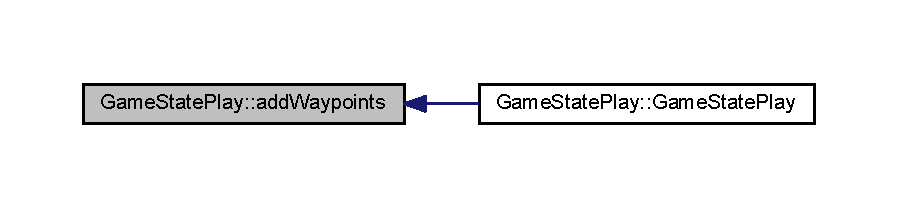
\includegraphics[width=350pt]{class_game_state_play_aee1a80f02dd69d8f06c041020eb4447e_icgraph}
\end{center}
\end{figure}


\hypertarget{class_game_state_play_a79237473ceeb26b94f641d0bf66c1ec0}{\index{Game\+State\+Play@{Game\+State\+Play}!button\+Command\+Library@{button\+Command\+Library}}
\index{button\+Command\+Library@{button\+Command\+Library}!Game\+State\+Play@{Game\+State\+Play}}
\subsubsection[{button\+Command\+Library}]{\setlength{\rightskip}{0pt plus 5cm}void Game\+State\+Play\+::button\+Command\+Library (
\begin{DoxyParamCaption}
{}
\end{DoxyParamCaption}
)\hspace{0.3cm}{\ttfamily [private]}}}\label{class_game_state_play_a79237473ceeb26b94f641d0bf66c1ec0}


Here is the call graph for this function\+:
\nopagebreak
\begin{figure}[H]
\begin{center}
\leavevmode
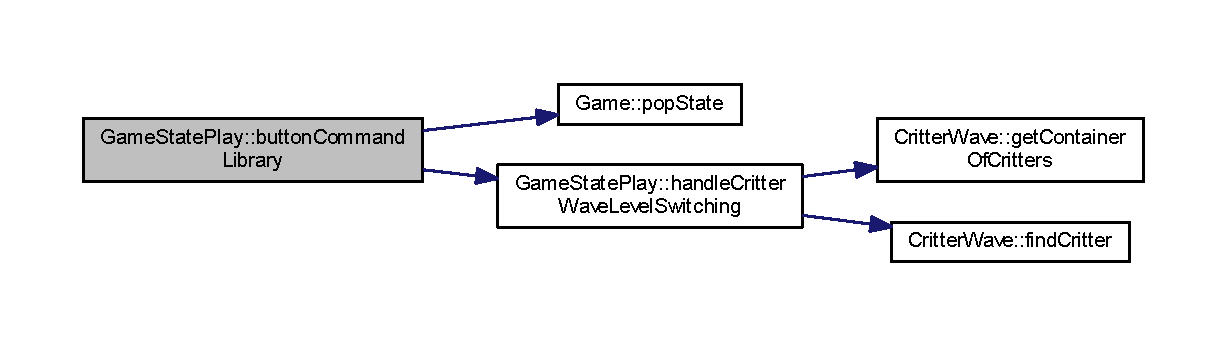
\includegraphics[width=350pt]{class_game_state_play_a79237473ceeb26b94f641d0bf66c1ec0_cgraph}
\end{center}
\end{figure}




Here is the caller graph for this function\+:\nopagebreak
\begin{figure}[H]
\begin{center}
\leavevmode
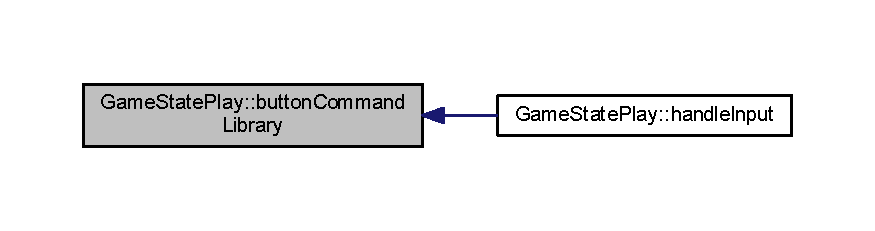
\includegraphics[width=350pt]{class_game_state_play_a79237473ceeb26b94f641d0bf66c1ec0_icgraph}
\end{center}
\end{figure}


\hypertarget{class_game_state_play_ac82134049ed6dd0aaa929e200f7185d5}{\index{Game\+State\+Play@{Game\+State\+Play}!check\+If\+At\+End\+Tile@{check\+If\+At\+End\+Tile}}
\index{check\+If\+At\+End\+Tile@{check\+If\+At\+End\+Tile}!Game\+State\+Play@{Game\+State\+Play}}
\subsubsection[{check\+If\+At\+End\+Tile}]{\setlength{\rightskip}{0pt plus 5cm}bool Game\+State\+Play\+::check\+If\+At\+End\+Tile (
\begin{DoxyParamCaption}
\item[{{\bf Critter} $\ast$}]{critter}
\end{DoxyParamCaption}
)\hspace{0.3cm}{\ttfamily [private]}}}\label{class_game_state_play_ac82134049ed6dd0aaa929e200f7185d5}


Here is the call graph for this function\+:
\nopagebreak
\begin{figure}[H]
\begin{center}
\leavevmode
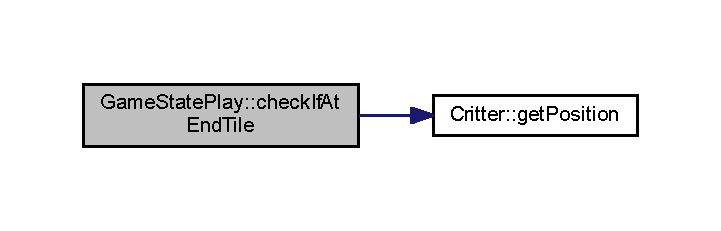
\includegraphics[width=350pt]{class_game_state_play_ac82134049ed6dd0aaa929e200f7185d5_cgraph}
\end{center}
\end{figure}




Here is the caller graph for this function\+:\nopagebreak
\begin{figure}[H]
\begin{center}
\leavevmode
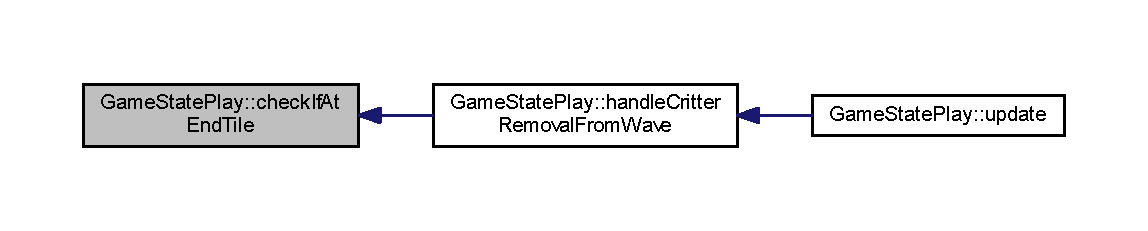
\includegraphics[width=350pt]{class_game_state_play_ac82134049ed6dd0aaa929e200f7185d5_icgraph}
\end{center}
\end{figure}


\hypertarget{class_game_state_play_a63a3ba0c891afd8ec126806bab4f315a}{\index{Game\+State\+Play@{Game\+State\+Play}!draw@{draw}}
\index{draw@{draw}!Game\+State\+Play@{Game\+State\+Play}}
\subsubsection[{draw}]{\setlength{\rightskip}{0pt plus 5cm}void Game\+State\+Play\+::draw (
\begin{DoxyParamCaption}
\item[{const float}]{delta\+\_\+time}
\end{DoxyParamCaption}
)\hspace{0.3cm}{\ttfamily [virtual]}}}\label{class_game_state_play_a63a3ba0c891afd8ec126806bab4f315a}


Draws game to the render window. 


\begin{DoxyParams}{Parameters}
{\em delta\+\_\+time} & Elapsed time during the game. \\
\hline
\end{DoxyParams}
\begin{DoxyReturn}{Returns}
Void.
\end{DoxyReturn}
This function sets the view to be drawn to the window, and draws everything related to state. 

Implements \hyperlink{class_game_state_a55a6a68aabdf7054ea0e6ddbf24902df}{Game\+State}.



Here is the call graph for this function\+:
\nopagebreak
\begin{figure}[H]
\begin{center}
\leavevmode
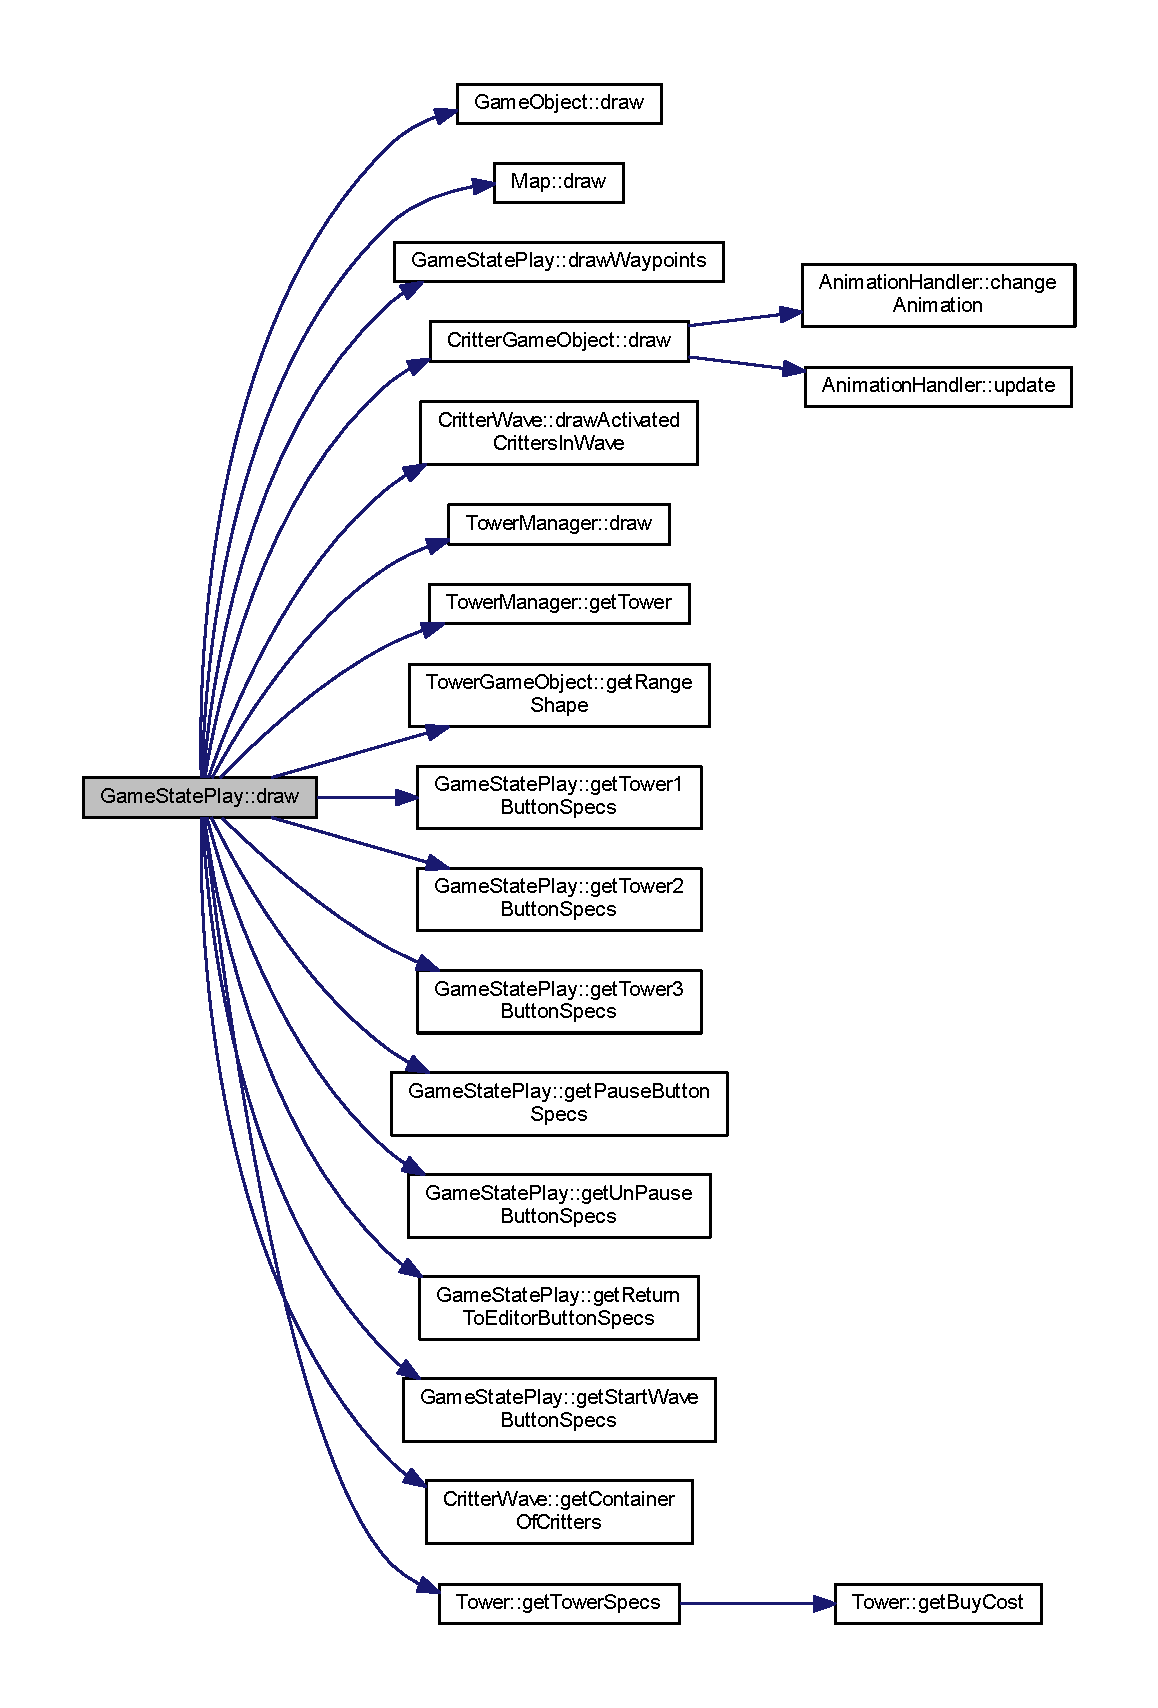
\includegraphics[width=350pt]{class_game_state_play_a63a3ba0c891afd8ec126806bab4f315a_cgraph}
\end{center}
\end{figure}




Here is the caller graph for this function\+:\nopagebreak
\begin{figure}[H]
\begin{center}
\leavevmode
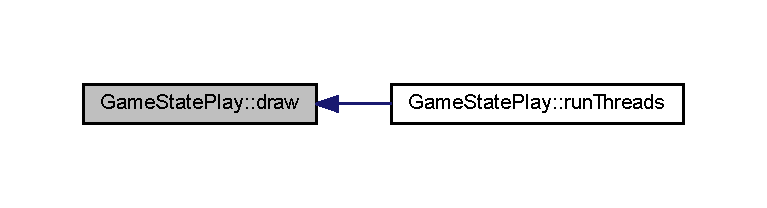
\includegraphics[width=350pt]{class_game_state_play_a63a3ba0c891afd8ec126806bab4f315a_icgraph}
\end{center}
\end{figure}


\hypertarget{class_game_state_play_a28fee46c0b9d0248ed319976be94494a}{\index{Game\+State\+Play@{Game\+State\+Play}!draw\+Waypoints@{draw\+Waypoints}}
\index{draw\+Waypoints@{draw\+Waypoints}!Game\+State\+Play@{Game\+State\+Play}}
\subsubsection[{draw\+Waypoints}]{\setlength{\rightskip}{0pt plus 5cm}void Game\+State\+Play\+::draw\+Waypoints (
\begin{DoxyParamCaption}
\item[{std\+::vector$<$ {\bf Waypoint} $>$}]{waypoints, }
\item[{sf\+::\+Render\+Window \&}]{game\+\_\+window}
\end{DoxyParamCaption}
)\hspace{0.3cm}{\ttfamily [private]}}}\label{class_game_state_play_a28fee46c0b9d0248ed319976be94494a}


Draw all waypoints. 

\begin{DoxyReturn}{Returns}
Void. 
\end{DoxyReturn}


Here is the caller graph for this function\+:\nopagebreak
\begin{figure}[H]
\begin{center}
\leavevmode
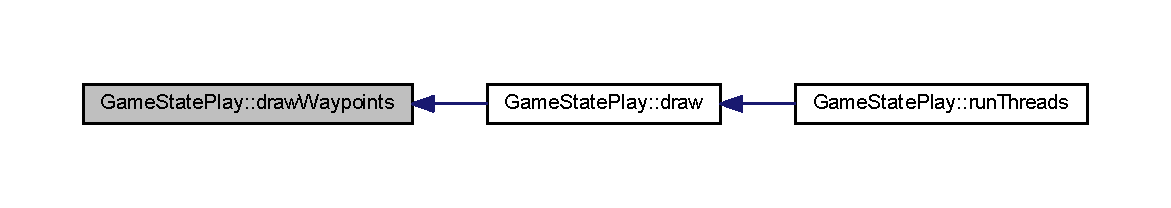
\includegraphics[width=350pt]{class_game_state_play_a28fee46c0b9d0248ed319976be94494a_icgraph}
\end{center}
\end{figure}


\hypertarget{class_game_state_play_a36f7d1ee2a500290e224a50f679ba3ff}{\index{Game\+State\+Play@{Game\+State\+Play}!get\+Current\+Critter\+Wave@{get\+Current\+Critter\+Wave}}
\index{get\+Current\+Critter\+Wave@{get\+Current\+Critter\+Wave}!Game\+State\+Play@{Game\+State\+Play}}
\subsubsection[{get\+Current\+Critter\+Wave}]{\setlength{\rightskip}{0pt plus 5cm}{\bf Critter\+Wave} $\ast$ Game\+State\+Play\+::get\+Current\+Critter\+Wave (
\begin{DoxyParamCaption}
{}
\end{DoxyParamCaption}
)}}\label{class_game_state_play_a36f7d1ee2a500290e224a50f679ba3ff}
\hypertarget{class_game_state_play_a84292b8af5919f8da3b54c1d1dba5cfd}{\index{Game\+State\+Play@{Game\+State\+Play}!get\+Pause\+Button\+Specs@{get\+Pause\+Button\+Specs}}
\index{get\+Pause\+Button\+Specs@{get\+Pause\+Button\+Specs}!Game\+State\+Play@{Game\+State\+Play}}
\subsubsection[{get\+Pause\+Button\+Specs}]{\setlength{\rightskip}{0pt plus 5cm}std\+::string Game\+State\+Play\+::get\+Pause\+Button\+Specs (
\begin{DoxyParamCaption}
{}
\end{DoxyParamCaption}
)\hspace{0.3cm}{\ttfamily [static]}, {\ttfamily [private]}}}\label{class_game_state_play_a84292b8af5919f8da3b54c1d1dba5cfd}


Here is the caller graph for this function\+:
\nopagebreak
\begin{figure}[H]
\begin{center}
\leavevmode
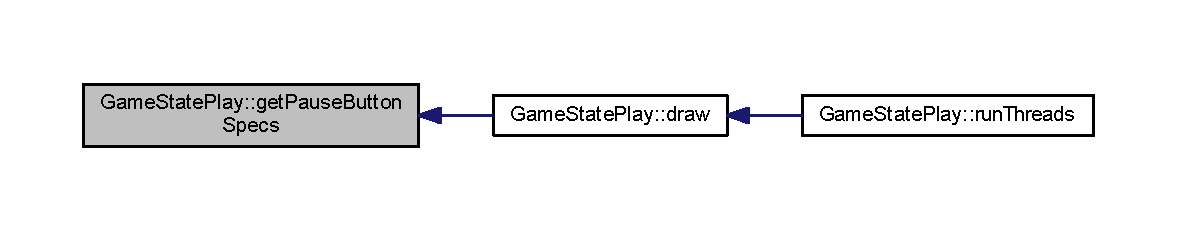
\includegraphics[width=350pt]{class_game_state_play_a84292b8af5919f8da3b54c1d1dba5cfd_icgraph}
\end{center}
\end{figure}


\hypertarget{class_game_state_play_aed4df6e7af126ba32ac06eb5dd79694d}{\index{Game\+State\+Play@{Game\+State\+Play}!get\+Return\+To\+Editor\+Button\+Specs@{get\+Return\+To\+Editor\+Button\+Specs}}
\index{get\+Return\+To\+Editor\+Button\+Specs@{get\+Return\+To\+Editor\+Button\+Specs}!Game\+State\+Play@{Game\+State\+Play}}
\subsubsection[{get\+Return\+To\+Editor\+Button\+Specs}]{\setlength{\rightskip}{0pt plus 5cm}std\+::string Game\+State\+Play\+::get\+Return\+To\+Editor\+Button\+Specs (
\begin{DoxyParamCaption}
{}
\end{DoxyParamCaption}
)\hspace{0.3cm}{\ttfamily [static]}, {\ttfamily [private]}}}\label{class_game_state_play_aed4df6e7af126ba32ac06eb5dd79694d}


Here is the caller graph for this function\+:
\nopagebreak
\begin{figure}[H]
\begin{center}
\leavevmode
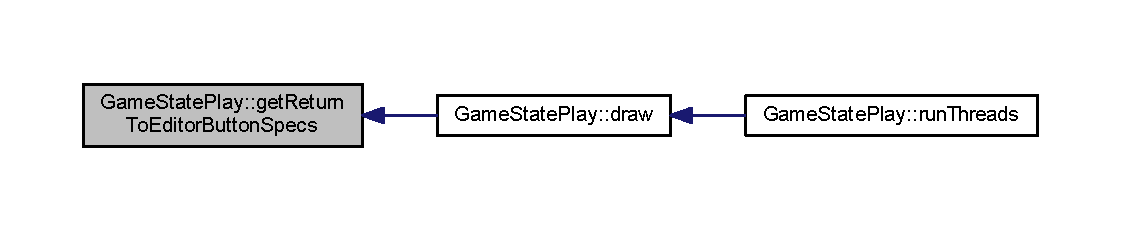
\includegraphics[width=350pt]{class_game_state_play_aed4df6e7af126ba32ac06eb5dd79694d_icgraph}
\end{center}
\end{figure}


\hypertarget{class_game_state_play_a6ebd21112217871afe2e0160f6eb0753}{\index{Game\+State\+Play@{Game\+State\+Play}!get\+Starting\+Waypoint@{get\+Starting\+Waypoint}}
\index{get\+Starting\+Waypoint@{get\+Starting\+Waypoint}!Game\+State\+Play@{Game\+State\+Play}}
\subsubsection[{get\+Starting\+Waypoint}]{\setlength{\rightskip}{0pt plus 5cm}{\bf Waypoint} $\ast$ Game\+State\+Play\+::get\+Starting\+Waypoint (
\begin{DoxyParamCaption}
{}
\end{DoxyParamCaption}
)}}\label{class_game_state_play_a6ebd21112217871afe2e0160f6eb0753}


Get starting waypoint. 

\begin{DoxyReturn}{Returns}
Vector containing \hyperlink{class_waypoint}{Waypoint} pointers. 
\end{DoxyReturn}


Here is the caller graph for this function\+:\nopagebreak
\begin{figure}[H]
\begin{center}
\leavevmode
\includegraphics[width=350pt]{class_game_state_play_a6ebd21112217871afe2e0160f6eb0753_icgraph}
\end{center}
\end{figure}


\hypertarget{class_game_state_play_ace72b0eb76edd4a7e02ab12454f9f5b7}{\index{Game\+State\+Play@{Game\+State\+Play}!get\+Start\+Wave\+Button\+Specs@{get\+Start\+Wave\+Button\+Specs}}
\index{get\+Start\+Wave\+Button\+Specs@{get\+Start\+Wave\+Button\+Specs}!Game\+State\+Play@{Game\+State\+Play}}
\subsubsection[{get\+Start\+Wave\+Button\+Specs}]{\setlength{\rightskip}{0pt plus 5cm}std\+::string Game\+State\+Play\+::get\+Start\+Wave\+Button\+Specs (
\begin{DoxyParamCaption}
{}
\end{DoxyParamCaption}
)\hspace{0.3cm}{\ttfamily [static]}, {\ttfamily [private]}}}\label{class_game_state_play_ace72b0eb76edd4a7e02ab12454f9f5b7}


Here is the caller graph for this function\+:
\nopagebreak
\begin{figure}[H]
\begin{center}
\leavevmode
\includegraphics[width=350pt]{class_game_state_play_ace72b0eb76edd4a7e02ab12454f9f5b7_icgraph}
\end{center}
\end{figure}


\hypertarget{class_game_state_play_a11c1d1976d85631c84a8db18b1458637}{\index{Game\+State\+Play@{Game\+State\+Play}!get\+Tower1\+Button\+Specs@{get\+Tower1\+Button\+Specs}}
\index{get\+Tower1\+Button\+Specs@{get\+Tower1\+Button\+Specs}!Game\+State\+Play@{Game\+State\+Play}}
\subsubsection[{get\+Tower1\+Button\+Specs}]{\setlength{\rightskip}{0pt plus 5cm}std\+::string Game\+State\+Play\+::get\+Tower1\+Button\+Specs (
\begin{DoxyParamCaption}
{}
\end{DoxyParamCaption}
)\hspace{0.3cm}{\ttfamily [static]}, {\ttfamily [private]}}}\label{class_game_state_play_a11c1d1976d85631c84a8db18b1458637}


Here is the caller graph for this function\+:
\nopagebreak
\begin{figure}[H]
\begin{center}
\leavevmode
\includegraphics[width=350pt]{class_game_state_play_a11c1d1976d85631c84a8db18b1458637_icgraph}
\end{center}
\end{figure}


\hypertarget{class_game_state_play_a0b9e886dc6a80b52f559441c7a3455d8}{\index{Game\+State\+Play@{Game\+State\+Play}!get\+Tower2\+Button\+Specs@{get\+Tower2\+Button\+Specs}}
\index{get\+Tower2\+Button\+Specs@{get\+Tower2\+Button\+Specs}!Game\+State\+Play@{Game\+State\+Play}}
\subsubsection[{get\+Tower2\+Button\+Specs}]{\setlength{\rightskip}{0pt plus 5cm}std\+::string Game\+State\+Play\+::get\+Tower2\+Button\+Specs (
\begin{DoxyParamCaption}
{}
\end{DoxyParamCaption}
)\hspace{0.3cm}{\ttfamily [static]}, {\ttfamily [private]}}}\label{class_game_state_play_a0b9e886dc6a80b52f559441c7a3455d8}


Here is the caller graph for this function\+:
\nopagebreak
\begin{figure}[H]
\begin{center}
\leavevmode
\includegraphics[width=350pt]{class_game_state_play_a0b9e886dc6a80b52f559441c7a3455d8_icgraph}
\end{center}
\end{figure}


\hypertarget{class_game_state_play_a0c79cb57b169ec8c0dc08c49451ebfc1}{\index{Game\+State\+Play@{Game\+State\+Play}!get\+Tower3\+Button\+Specs@{get\+Tower3\+Button\+Specs}}
\index{get\+Tower3\+Button\+Specs@{get\+Tower3\+Button\+Specs}!Game\+State\+Play@{Game\+State\+Play}}
\subsubsection[{get\+Tower3\+Button\+Specs}]{\setlength{\rightskip}{0pt plus 5cm}std\+::string Game\+State\+Play\+::get\+Tower3\+Button\+Specs (
\begin{DoxyParamCaption}
{}
\end{DoxyParamCaption}
)\hspace{0.3cm}{\ttfamily [static]}, {\ttfamily [private]}}}\label{class_game_state_play_a0c79cb57b169ec8c0dc08c49451ebfc1}


Here is the caller graph for this function\+:
\nopagebreak
\begin{figure}[H]
\begin{center}
\leavevmode
\includegraphics[width=350pt]{class_game_state_play_a0c79cb57b169ec8c0dc08c49451ebfc1_icgraph}
\end{center}
\end{figure}


\hypertarget{class_game_state_play_a93771d14333ebc475f2428d3c1a3c3d3}{\index{Game\+State\+Play@{Game\+State\+Play}!get\+Un\+Pause\+Button\+Specs@{get\+Un\+Pause\+Button\+Specs}}
\index{get\+Un\+Pause\+Button\+Specs@{get\+Un\+Pause\+Button\+Specs}!Game\+State\+Play@{Game\+State\+Play}}
\subsubsection[{get\+Un\+Pause\+Button\+Specs}]{\setlength{\rightskip}{0pt plus 5cm}std\+::string Game\+State\+Play\+::get\+Un\+Pause\+Button\+Specs (
\begin{DoxyParamCaption}
{}
\end{DoxyParamCaption}
)\hspace{0.3cm}{\ttfamily [static]}, {\ttfamily [private]}}}\label{class_game_state_play_a93771d14333ebc475f2428d3c1a3c3d3}


Here is the caller graph for this function\+:
\nopagebreak
\begin{figure}[H]
\begin{center}
\leavevmode
\includegraphics[width=350pt]{class_game_state_play_a93771d14333ebc475f2428d3c1a3c3d3_icgraph}
\end{center}
\end{figure}


\hypertarget{class_game_state_play_aae84ae33a68caa8bf05a4a2a49a2b41d}{\index{Game\+State\+Play@{Game\+State\+Play}!get\+Waypoints\+From\+Map\+Path@{get\+Waypoints\+From\+Map\+Path}}
\index{get\+Waypoints\+From\+Map\+Path@{get\+Waypoints\+From\+Map\+Path}!Game\+State\+Play@{Game\+State\+Play}}
\subsubsection[{get\+Waypoints\+From\+Map\+Path}]{\setlength{\rightskip}{0pt plus 5cm}std\+::vector$<$ sf\+::\+Vector2f $>$ Game\+State\+Play\+::get\+Waypoints\+From\+Map\+Path (
\begin{DoxyParamCaption}
{}
\end{DoxyParamCaption}
)\hspace{0.3cm}{\ttfamily [private]}}}\label{class_game_state_play_aae84ae33a68caa8bf05a4a2a49a2b41d}


Create waypoint vector from the map's path. 

\begin{DoxyReturn}{Returns}
Vector containing positions. 
\end{DoxyReturn}


Here is the call graph for this function\+:\nopagebreak
\begin{figure}[H]
\begin{center}
\leavevmode
\includegraphics[width=350pt]{class_game_state_play_aae84ae33a68caa8bf05a4a2a49a2b41d_cgraph}
\end{center}
\end{figure}




Here is the caller graph for this function\+:\nopagebreak
\begin{figure}[H]
\begin{center}
\leavevmode
\includegraphics[width=350pt]{class_game_state_play_aae84ae33a68caa8bf05a4a2a49a2b41d_icgraph}
\end{center}
\end{figure}


\hypertarget{class_game_state_play_a2278751d53b50beb97c809db26f1b9b6}{\index{Game\+State\+Play@{Game\+State\+Play}!handle\+Critter\+Removal\+From\+Wave@{handle\+Critter\+Removal\+From\+Wave}}
\index{handle\+Critter\+Removal\+From\+Wave@{handle\+Critter\+Removal\+From\+Wave}!Game\+State\+Play@{Game\+State\+Play}}
\subsubsection[{handle\+Critter\+Removal\+From\+Wave}]{\setlength{\rightskip}{0pt plus 5cm}void Game\+State\+Play\+::handle\+Critter\+Removal\+From\+Wave (
\begin{DoxyParamCaption}
{}
\end{DoxyParamCaption}
)\hspace{0.3cm}{\ttfamily [private]}}}\label{class_game_state_play_a2278751d53b50beb97c809db26f1b9b6}


Here is the call graph for this function\+:
\nopagebreak
\begin{figure}[H]
\begin{center}
\leavevmode
\includegraphics[width=350pt]{class_game_state_play_a2278751d53b50beb97c809db26f1b9b6_cgraph}
\end{center}
\end{figure}




Here is the caller graph for this function\+:\nopagebreak
\begin{figure}[H]
\begin{center}
\leavevmode
\includegraphics[width=350pt]{class_game_state_play_a2278751d53b50beb97c809db26f1b9b6_icgraph}
\end{center}
\end{figure}


\hypertarget{class_game_state_play_a2eda31c4d98a8440c6eba38604aa2a79}{\index{Game\+State\+Play@{Game\+State\+Play}!handle\+Critter\+Wave\+Level\+Switching@{handle\+Critter\+Wave\+Level\+Switching}}
\index{handle\+Critter\+Wave\+Level\+Switching@{handle\+Critter\+Wave\+Level\+Switching}!Game\+State\+Play@{Game\+State\+Play}}
\subsubsection[{handle\+Critter\+Wave\+Level\+Switching}]{\setlength{\rightskip}{0pt plus 5cm}void Game\+State\+Play\+::handle\+Critter\+Wave\+Level\+Switching (
\begin{DoxyParamCaption}
{}
\end{DoxyParamCaption}
)\hspace{0.3cm}{\ttfamily [private]}}}\label{class_game_state_play_a2eda31c4d98a8440c6eba38604aa2a79}


Here is the call graph for this function\+:\nopagebreak
\begin{figure}[H]
\begin{center}
\leavevmode
\includegraphics[width=350pt]{class_game_state_play_a2eda31c4d98a8440c6eba38604aa2a79_cgraph}
\end{center}
\end{figure}




Here is the caller graph for this function\+:\nopagebreak
\begin{figure}[H]
\begin{center}
\leavevmode
\includegraphics[width=350pt]{class_game_state_play_a2eda31c4d98a8440c6eba38604aa2a79_icgraph}
\end{center}
\end{figure}


\hypertarget{class_game_state_play_aec5f72cea0e80d1d83b9cbe155a65ce9}{\index{Game\+State\+Play@{Game\+State\+Play}!handle\+Game\+Over@{handle\+Game\+Over}}
\index{handle\+Game\+Over@{handle\+Game\+Over}!Game\+State\+Play@{Game\+State\+Play}}
\subsubsection[{handle\+Game\+Over}]{\setlength{\rightskip}{0pt plus 5cm}void Game\+State\+Play\+::handle\+Game\+Over (
\begin{DoxyParamCaption}
{}
\end{DoxyParamCaption}
)}}\label{class_game_state_play_aec5f72cea0e80d1d83b9cbe155a65ce9}


Here is the call graph for this function\+:\nopagebreak
\begin{figure}[H]
\begin{center}
\leavevmode
\includegraphics[width=350pt]{class_game_state_play_aec5f72cea0e80d1d83b9cbe155a65ce9_cgraph}
\end{center}
\end{figure}




Here is the caller graph for this function\+:\nopagebreak
\begin{figure}[H]
\begin{center}
\leavevmode
\includegraphics[width=350pt]{class_game_state_play_aec5f72cea0e80d1d83b9cbe155a65ce9_icgraph}
\end{center}
\end{figure}


\hypertarget{class_game_state_play_ae9acc781e1fdbc931784ba3892c469ce}{\index{Game\+State\+Play@{Game\+State\+Play}!handle\+Input@{handle\+Input}}
\index{handle\+Input@{handle\+Input}!Game\+State\+Play@{Game\+State\+Play}}
\subsubsection[{handle\+Input}]{\setlength{\rightskip}{0pt plus 5cm}void Game\+State\+Play\+::handle\+Input (
\begin{DoxyParamCaption}
{}
\end{DoxyParamCaption}
)\hspace{0.3cm}{\ttfamily [virtual]}}}\label{class_game_state_play_ae9acc781e1fdbc931784ba3892c469ce}


Handles player input. 

\begin{DoxyReturn}{Returns}
Void. 
\end{DoxyReturn}
Close the window 

Implements \hyperlink{class_game_state_a970b55edd5a1da31ea0f7113e2c1f85a}{Game\+State}.



Here is the call graph for this function\+:
\nopagebreak
\begin{figure}[H]
\begin{center}
\leavevmode
\includegraphics[height=550pt]{class_game_state_play_ae9acc781e1fdbc931784ba3892c469ce_cgraph}
\end{center}
\end{figure}


\hypertarget{class_game_state_play_a3a6947bfe8be3d1974094acb8362eda9}{\index{Game\+State\+Play@{Game\+State\+Play}!initialize\+Button\+Map@{initialize\+Button\+Map}}
\index{initialize\+Button\+Map@{initialize\+Button\+Map}!Game\+State\+Play@{Game\+State\+Play}}
\subsubsection[{initialize\+Button\+Map}]{\setlength{\rightskip}{0pt plus 5cm}void Game\+State\+Play\+::initialize\+Button\+Map (
\begin{DoxyParamCaption}
{}
\end{DoxyParamCaption}
)\hspace{0.3cm}{\ttfamily [private]}}}\label{class_game_state_play_a3a6947bfe8be3d1974094acb8362eda9}


Here is the call graph for this function\+:\nopagebreak
\begin{figure}[H]
\begin{center}
\leavevmode
\includegraphics[width=350pt]{class_game_state_play_a3a6947bfe8be3d1974094acb8362eda9_cgraph}
\end{center}
\end{figure}




Here is the caller graph for this function\+:\nopagebreak
\begin{figure}[H]
\begin{center}
\leavevmode
\includegraphics[width=350pt]{class_game_state_play_a3a6947bfe8be3d1974094acb8362eda9_icgraph}
\end{center}
\end{figure}


\hypertarget{class_game_state_play_ae812a7447027abe5fcc2f79bf3e35ad8}{\index{Game\+State\+Play@{Game\+State\+Play}!move\+Activated\+Critters@{move\+Activated\+Critters}}
\index{move\+Activated\+Critters@{move\+Activated\+Critters}!Game\+State\+Play@{Game\+State\+Play}}
\subsubsection[{move\+Activated\+Critters}]{\setlength{\rightskip}{0pt plus 5cm}void Game\+State\+Play\+::move\+Activated\+Critters (
\begin{DoxyParamCaption}
\item[{const float}]{delta\+\_\+time}
\end{DoxyParamCaption}
)\hspace{0.3cm}{\ttfamily [private]}}}\label{class_game_state_play_ae812a7447027abe5fcc2f79bf3e35ad8}


Here is the call graph for this function\+:
\nopagebreak
\begin{figure}[H]
\begin{center}
\leavevmode
\includegraphics[width=350pt]{class_game_state_play_ae812a7447027abe5fcc2f79bf3e35ad8_cgraph}
\end{center}
\end{figure}




Here is the caller graph for this function\+:\nopagebreak
\begin{figure}[H]
\begin{center}
\leavevmode
\includegraphics[width=350pt]{class_game_state_play_ae812a7447027abe5fcc2f79bf3e35ad8_icgraph}
\end{center}
\end{figure}


\hypertarget{class_game_state_play_a0d6ff2e65992c5fb29f180c6b1eb9435}{\index{Game\+State\+Play@{Game\+State\+Play}!move\+Critter@{move\+Critter}}
\index{move\+Critter@{move\+Critter}!Game\+State\+Play@{Game\+State\+Play}}
\subsubsection[{move\+Critter}]{\setlength{\rightskip}{0pt plus 5cm}void Game\+State\+Play\+::move\+Critter (
\begin{DoxyParamCaption}
\item[{{\bf Critter} $\ast$}]{critter, }
\item[{const float}]{delta\+\_\+time}
\end{DoxyParamCaption}
)\hspace{0.3cm}{\ttfamily [private]}}}\label{class_game_state_play_a0d6ff2e65992c5fb29f180c6b1eb9435}


Here is the call graph for this function\+:
\nopagebreak
\begin{figure}[H]
\begin{center}
\leavevmode
\includegraphics[width=350pt]{class_game_state_play_a0d6ff2e65992c5fb29f180c6b1eb9435_cgraph}
\end{center}
\end{figure}




Here is the caller graph for this function\+:\nopagebreak
\begin{figure}[H]
\begin{center}
\leavevmode
\includegraphics[width=350pt]{class_game_state_play_a0d6ff2e65992c5fb29f180c6b1eb9435_icgraph}
\end{center}
\end{figure}


\hypertarget{class_game_state_play_a5076f9d4d81b1b9dc4e71c627f40a9d2}{\index{Game\+State\+Play@{Game\+State\+Play}!register\+Observer@{register\+Observer}}
\index{register\+Observer@{register\+Observer}!Game\+State\+Play@{Game\+State\+Play}}
\subsubsection[{register\+Observer}]{\setlength{\rightskip}{0pt plus 5cm}void Game\+State\+Play\+::register\+Observer (
\begin{DoxyParamCaption}
\item[{{\bf Tower} $\ast$}]{tower}
\end{DoxyParamCaption}
)}}\label{class_game_state_play_a5076f9d4d81b1b9dc4e71c627f40a9d2}
\hypertarget{class_game_state_play_ab41594c10b04429a3126d4a8085de82d}{\index{Game\+State\+Play@{Game\+State\+Play}!run\+Threads@{run\+Threads}}
\index{run\+Threads@{run\+Threads}!Game\+State\+Play@{Game\+State\+Play}}
\subsubsection[{run\+Threads}]{\setlength{\rightskip}{0pt plus 5cm}void Game\+State\+Play\+::run\+Threads (
\begin{DoxyParamCaption}
{}
\end{DoxyParamCaption}
)\hspace{0.3cm}{\ttfamily [virtual]}}}\label{class_game_state_play_ab41594c10b04429a3126d4a8085de82d}


Implements \hyperlink{class_game_state_a98cd49f1d8fd9fc3e79d607a238ba518}{Game\+State}.



Here is the call graph for this function\+:
\nopagebreak
\begin{figure}[H]
\begin{center}
\leavevmode
\includegraphics[width=350pt]{class_game_state_play_ab41594c10b04429a3126d4a8085de82d_cgraph}
\end{center}
\end{figure}


\hypertarget{class_game_state_play_a6047cbdce7daa2092d95bf786db5267a}{\index{Game\+State\+Play@{Game\+State\+Play}!set\+Critter\+Wave\+Levels@{set\+Critter\+Wave\+Levels}}
\index{set\+Critter\+Wave\+Levels@{set\+Critter\+Wave\+Levels}!Game\+State\+Play@{Game\+State\+Play}}
\subsubsection[{set\+Critter\+Wave\+Levels}]{\setlength{\rightskip}{0pt plus 5cm}void Game\+State\+Play\+::set\+Critter\+Wave\+Levels (
\begin{DoxyParamCaption}
\item[{{\bf Waypoint} $\ast$}]{starting\+\_\+waypoint}
\end{DoxyParamCaption}
)\hspace{0.3cm}{\ttfamily [private]}}}\label{class_game_state_play_a6047cbdce7daa2092d95bf786db5267a}


Here is the call graph for this function\+:\nopagebreak
\begin{figure}[H]
\begin{center}
\leavevmode
\includegraphics[width=350pt]{class_game_state_play_a6047cbdce7daa2092d95bf786db5267a_cgraph}
\end{center}
\end{figure}




Here is the caller graph for this function\+:\nopagebreak
\begin{figure}[H]
\begin{center}
\leavevmode
\includegraphics[width=350pt]{class_game_state_play_a6047cbdce7daa2092d95bf786db5267a_icgraph}
\end{center}
\end{figure}


\hypertarget{class_game_state_play_ab33de76aa28534d14aa1d79bed43aa17}{\index{Game\+State\+Play@{Game\+State\+Play}!tower\+Command\+Library@{tower\+Command\+Library}}
\index{tower\+Command\+Library@{tower\+Command\+Library}!Game\+State\+Play@{Game\+State\+Play}}
\subsubsection[{tower\+Command\+Library}]{\setlength{\rightskip}{0pt plus 5cm}void Game\+State\+Play\+::tower\+Command\+Library (
\begin{DoxyParamCaption}
\item[{const int}]{tile\+X, }
\item[{const int}]{tile\+Y}
\end{DoxyParamCaption}
)\hspace{0.3cm}{\ttfamily [private]}}}\label{class_game_state_play_ab33de76aa28534d14aa1d79bed43aa17}


Here is the call graph for this function\+:
\nopagebreak
\begin{figure}[H]
\begin{center}
\leavevmode
\includegraphics[width=350pt]{class_game_state_play_ab33de76aa28534d14aa1d79bed43aa17_cgraph}
\end{center}
\end{figure}




Here is the caller graph for this function\+:\nopagebreak
\begin{figure}[H]
\begin{center}
\leavevmode
\includegraphics[width=350pt]{class_game_state_play_ab33de76aa28534d14aa1d79bed43aa17_icgraph}
\end{center}
\end{figure}


\hypertarget{class_game_state_play_a2faf041a447ddf86726658455560abb8}{\index{Game\+State\+Play@{Game\+State\+Play}!update@{update}}
\index{update@{update}!Game\+State\+Play@{Game\+State\+Play}}
\subsubsection[{update}]{\setlength{\rightskip}{0pt plus 5cm}void Game\+State\+Play\+::update (
\begin{DoxyParamCaption}
\item[{const float}]{delta\+\_\+time}
\end{DoxyParamCaption}
)\hspace{0.3cm}{\ttfamily [virtual]}}}\label{class_game_state_play_a2faf041a447ddf86726658455560abb8}


Updates game changes. 


\begin{DoxyParams}{Parameters}
{\em delta\+\_\+time} & Elapsed time during the game. \\
\hline
\end{DoxyParams}
\begin{DoxyReturn}{Returns}
Void. 
\end{DoxyReturn}


Implements \hyperlink{class_game_state_ad331d02d3989271b8cbc88fcb1448959}{Game\+State}.



Here is the call graph for this function\+:
\nopagebreak
\begin{figure}[H]
\begin{center}
\leavevmode
\includegraphics[width=350pt]{class_game_state_play_a2faf041a447ddf86726658455560abb8_cgraph}
\end{center}
\end{figure}




\subsection{Member Data Documentation}
\hypertarget{class_game_state_play_a3f05ff560a8dbeb5a1922e23c6bbff72}{\index{Game\+State\+Play@{Game\+State\+Play}!\+\_\+game\+\_\+object\+\_\+manager@{\+\_\+game\+\_\+object\+\_\+manager}}
\index{\+\_\+game\+\_\+object\+\_\+manager@{\+\_\+game\+\_\+object\+\_\+manager}!Game\+State\+Play@{Game\+State\+Play}}
\subsubsection[{\+\_\+game\+\_\+object\+\_\+manager}]{\setlength{\rightskip}{0pt plus 5cm}{\bf Game\+Object\+Manager} Game\+State\+Play\+::\+\_\+game\+\_\+object\+\_\+manager\hspace{0.3cm}{\ttfamily [static]}, {\ttfamily [private]}}}\label{class_game_state_play_a3f05ff560a8dbeb5a1922e23c6bbff72}
\hypertarget{class_game_state_play_a9513cfeac2178d83e23ba6f9291fba8c}{\index{Game\+State\+Play@{Game\+State\+Play}!\+\_\+game\+View@{\+\_\+game\+View}}
\index{\+\_\+game\+View@{\+\_\+game\+View}!Game\+State\+Play@{Game\+State\+Play}}
\subsubsection[{\+\_\+game\+View}]{\setlength{\rightskip}{0pt plus 5cm}sf\+::\+View Game\+State\+Play\+::\+\_\+game\+View\hspace{0.3cm}{\ttfamily [private]}}}\label{class_game_state_play_a9513cfeac2178d83e23ba6f9291fba8c}


Camera view for the gameplay displayed to the window. 

\hypertarget{class_game_state_play_affee804e287fd1968fe8c5b0a303b05d}{\index{Game\+State\+Play@{Game\+State\+Play}!\+\_\+gui\+View@{\+\_\+gui\+View}}
\index{\+\_\+gui\+View@{\+\_\+gui\+View}!Game\+State\+Play@{Game\+State\+Play}}
\subsubsection[{\+\_\+gui\+View}]{\setlength{\rightskip}{0pt plus 5cm}sf\+::\+View Game\+State\+Play\+::\+\_\+gui\+View\hspace{0.3cm}{\ttfamily [private]}}}\label{class_game_state_play_affee804e287fd1968fe8c5b0a303b05d}


Camera view for the H\+U\+D displayed to the window. 

\hypertarget{class_game_state_play_ace195ef46750d243d3bbaf2abaaf6e2e}{\index{Game\+State\+Play@{Game\+State\+Play}!blacky@{blacky}}
\index{blacky@{blacky}!Game\+State\+Play@{Game\+State\+Play}}
\subsubsection[{blacky}]{\setlength{\rightskip}{0pt plus 5cm}{\bf Black\+Cat}$\ast$ Game\+State\+Play\+::blacky}}\label{class_game_state_play_ace195ef46750d243d3bbaf2abaaf6e2e}
\hypertarget{class_game_state_play_ab0755d9a7eb5708a840d82bbdc7eb9f2}{\index{Game\+State\+Play@{Game\+State\+Play}!button\+Map@{button\+Map}}
\index{button\+Map@{button\+Map}!Game\+State\+Play@{Game\+State\+Play}}
\subsubsection[{button\+Map}]{\setlength{\rightskip}{0pt plus 5cm}std\+::map$<$string,{\bf Game\+Object}$>$ Game\+State\+Play\+::button\+Map\hspace{0.3cm}{\ttfamily [private]}}}\label{class_game_state_play_ab0755d9a7eb5708a840d82bbdc7eb9f2}
\hypertarget{class_game_state_play_a65d1a4d74f886ce3de872c1ffbb63d57}{\index{Game\+State\+Play@{Game\+State\+Play}!button\+Specs@{button\+Specs}}
\index{button\+Specs@{button\+Specs}!Game\+State\+Play@{Game\+State\+Play}}
\subsubsection[{button\+Specs}]{\setlength{\rightskip}{0pt plus 5cm}sf\+::\+Text Game\+State\+Play\+::button\+Specs\hspace{0.3cm}{\ttfamily [private]}}}\label{class_game_state_play_a65d1a4d74f886ce3de872c1ffbb63d57}
\hypertarget{class_game_state_play_a7ca10b4aceefc0e2732ec427c5b5b5c5}{\index{Game\+State\+Play@{Game\+State\+Play}!critter\+Health@{critter\+Health}}
\index{critter\+Health@{critter\+Health}!Game\+State\+Play@{Game\+State\+Play}}
\subsubsection[{critter\+Health}]{\setlength{\rightskip}{0pt plus 5cm}std\+::map$<$int,sf\+::\+Text$>$ Game\+State\+Play\+::critter\+Health\hspace{0.3cm}{\ttfamily [private]}}}\label{class_game_state_play_a7ca10b4aceefc0e2732ec427c5b5b5c5}
\hypertarget{class_game_state_play_a1667ea17be43ded7176a9dc28d99a8e1}{\index{Game\+State\+Play@{Game\+State\+Play}!critter\+Specs@{critter\+Specs}}
\index{critter\+Specs@{critter\+Specs}!Game\+State\+Play@{Game\+State\+Play}}
\subsubsection[{critter\+Specs}]{\setlength{\rightskip}{0pt plus 5cm}sf\+::\+Text Game\+State\+Play\+::critter\+Specs\hspace{0.3cm}{\ttfamily [private]}}}\label{class_game_state_play_a1667ea17be43ded7176a9dc28d99a8e1}
\hypertarget{class_game_state_play_a64cd6841a6f7139ff7e3747e4159654c}{\index{Game\+State\+Play@{Game\+State\+Play}!current\+\_\+wave@{current\+\_\+wave}}
\index{current\+\_\+wave@{current\+\_\+wave}!Game\+State\+Play@{Game\+State\+Play}}
\subsubsection[{current\+\_\+wave}]{\setlength{\rightskip}{0pt plus 5cm}{\bf Critter\+Wave}$\ast$ Game\+State\+Play\+::current\+\_\+wave\hspace{0.3cm}{\ttfamily [private]}}}\label{class_game_state_play_a64cd6841a6f7139ff7e3747e4159654c}
\hypertarget{class_game_state_play_a14914e609fd8b83324b3fc47343ec19a}{\index{Game\+State\+Play@{Game\+State\+Play}!current\+\_\+waypoints@{current\+\_\+waypoints}}
\index{current\+\_\+waypoints@{current\+\_\+waypoints}!Game\+State\+Play@{Game\+State\+Play}}
\subsubsection[{current\+\_\+waypoints}]{\setlength{\rightskip}{0pt plus 5cm}std\+::vector$<${\bf Waypoint}$>$ Game\+State\+Play\+::current\+\_\+waypoints\hspace{0.3cm}{\ttfamily [private]}}}\label{class_game_state_play_a14914e609fd8b83324b3fc47343ec19a}
\hypertarget{class_game_state_play_aa0948c192d3ef1adb6eaaeade8521733}{\index{Game\+State\+Play@{Game\+State\+Play}!delay\+\_\+count@{delay\+\_\+count}}
\index{delay\+\_\+count@{delay\+\_\+count}!Game\+State\+Play@{Game\+State\+Play}}
\subsubsection[{delay\+\_\+count}]{\setlength{\rightskip}{0pt plus 5cm}int Game\+State\+Play\+::delay\+\_\+count}}\label{class_game_state_play_aa0948c192d3ef1adb6eaaeade8521733}
\hypertarget{class_game_state_play_aac5b1d9de4ab0ad2445d97a588cb3168}{\index{Game\+State\+Play@{Game\+State\+Play}!draw\+Thread@{draw\+Thread}}
\index{draw\+Thread@{draw\+Thread}!Game\+State\+Play@{Game\+State\+Play}}
\subsubsection[{draw\+Thread}]{\setlength{\rightskip}{0pt plus 5cm}std\+::thread Game\+State\+Play\+::draw\+Thread}}\label{class_game_state_play_aac5b1d9de4ab0ad2445d97a588cb3168}
\hypertarget{class_game_state_play_a2c0118859e607a1ef2aa008f1b94b7f8}{\index{Game\+State\+Play@{Game\+State\+Play}!effect\+Damage@{effect\+Damage}}
\index{effect\+Damage@{effect\+Damage}!Game\+State\+Play@{Game\+State\+Play}}
\subsubsection[{effect\+Damage}]{\setlength{\rightskip}{0pt plus 5cm}std\+::map$<$int,sf\+::\+Text$>$ Game\+State\+Play\+::effect\+Damage\hspace{0.3cm}{\ttfamily [private]}}}\label{class_game_state_play_a2c0118859e607a1ef2aa008f1b94b7f8}
\hypertarget{class_game_state_play_a672216db210bc2dca82196badc7c20e9}{\index{Game\+State\+Play@{Game\+State\+Play}!effect\+Damage\+Clock@{effect\+Damage\+Clock}}
\index{effect\+Damage\+Clock@{effect\+Damage\+Clock}!Game\+State\+Play@{Game\+State\+Play}}
\subsubsection[{effect\+Damage\+Clock}]{\setlength{\rightskip}{0pt plus 5cm}std\+::map$<$int,sf\+::\+Clock$>$ Game\+State\+Play\+::effect\+Damage\+Clock\hspace{0.3cm}{\ttfamily [private]}}}\label{class_game_state_play_a672216db210bc2dca82196badc7c20e9}
\hypertarget{class_game_state_play_a9d324dec79041681951cf84349507e7f}{\index{Game\+State\+Play@{Game\+State\+Play}!effect\+Damage\+Time@{effect\+Damage\+Time}}
\index{effect\+Damage\+Time@{effect\+Damage\+Time}!Game\+State\+Play@{Game\+State\+Play}}
\subsubsection[{effect\+Damage\+Time}]{\setlength{\rightskip}{0pt plus 5cm}sf\+::\+Time Game\+State\+Play\+::effect\+Damage\+Time\hspace{0.3cm}{\ttfamily [private]}}}\label{class_game_state_play_a9d324dec79041681951cf84349507e7f}
\hypertarget{class_game_state_play_a0e613be489b2c61857676303a15ce3cc}{\index{Game\+State\+Play@{Game\+State\+Play}!end\+Of\+Waves@{end\+Of\+Waves}}
\index{end\+Of\+Waves@{end\+Of\+Waves}!Game\+State\+Play@{Game\+State\+Play}}
\subsubsection[{end\+Of\+Waves}]{\setlength{\rightskip}{0pt plus 5cm}bool Game\+State\+Play\+::end\+Of\+Waves}}\label{class_game_state_play_a0e613be489b2c61857676303a15ce3cc}
\hypertarget{class_game_state_play_a6b8fba9f1816c183dc546ccbe8fc04cc}{\index{Game\+State\+Play@{Game\+State\+Play}!fastest@{fastest}}
\index{fastest@{fastest}!Game\+State\+Play@{Game\+State\+Play}}
\subsubsection[{fastest}]{\setlength{\rightskip}{0pt plus 5cm}sf\+::\+Text Game\+State\+Play\+::fastest\hspace{0.3cm}{\ttfamily [private]}}}\label{class_game_state_play_a6b8fba9f1816c183dc546ccbe8fc04cc}
\hypertarget{class_game_state_play_af37399cc10da66842740622a891489e0}{\index{Game\+State\+Play@{Game\+State\+Play}!field\+Tower\+Selector@{field\+Tower\+Selector}}
\index{field\+Tower\+Selector@{field\+Tower\+Selector}!Game\+State\+Play@{Game\+State\+Play}}
\subsubsection[{field\+Tower\+Selector}]{\setlength{\rightskip}{0pt plus 5cm}{\bf Tower}$\ast$ Game\+State\+Play\+::field\+Tower\+Selector\hspace{0.3cm}{\ttfamily [private]}}}\label{class_game_state_play_af37399cc10da66842740622a891489e0}
\hypertarget{class_game_state_play_a59cc893637827eb0d9ee902262548980}{\index{Game\+State\+Play@{Game\+State\+Play}!first\+Start@{first\+Start}}
\index{first\+Start@{first\+Start}!Game\+State\+Play@{Game\+State\+Play}}
\subsubsection[{first\+Start}]{\setlength{\rightskip}{0pt plus 5cm}bool Game\+State\+Play\+::first\+Start}}\label{class_game_state_play_a59cc893637827eb0d9ee902262548980}
\hypertarget{class_game_state_play_a333494e6c4a8ae4a285635776c3b486e}{\index{Game\+State\+Play@{Game\+State\+Play}!font@{font}}
\index{font@{font}!Game\+State\+Play@{Game\+State\+Play}}
\subsubsection[{font}]{\setlength{\rightskip}{0pt plus 5cm}sf\+::\+Font Game\+State\+Play\+::font\hspace{0.3cm}{\ttfamily [private]}}}\label{class_game_state_play_a333494e6c4a8ae4a285635776c3b486e}
\hypertarget{class_game_state_play_af65d40be0eb5748b1d80186cefd3cc71}{\index{Game\+State\+Play@{Game\+State\+Play}!health\+Clock@{health\+Clock}}
\index{health\+Clock@{health\+Clock}!Game\+State\+Play@{Game\+State\+Play}}
\subsubsection[{health\+Clock}]{\setlength{\rightskip}{0pt plus 5cm}std\+::map$<$int,sf\+::\+Clock$>$ Game\+State\+Play\+::health\+Clock\hspace{0.3cm}{\ttfamily [private]}}}\label{class_game_state_play_af65d40be0eb5748b1d80186cefd3cc71}
\hypertarget{class_game_state_play_a4a2fd0f59504ad64f5d8b871cbf3cd35}{\index{Game\+State\+Play@{Game\+State\+Play}!health\+Time@{health\+Time}}
\index{health\+Time@{health\+Time}!Game\+State\+Play@{Game\+State\+Play}}
\subsubsection[{health\+Time}]{\setlength{\rightskip}{0pt plus 5cm}sf\+::\+Time Game\+State\+Play\+::health\+Time\hspace{0.3cm}{\ttfamily [private]}}}\label{class_game_state_play_a4a2fd0f59504ad64f5d8b871cbf3cd35}
\hypertarget{class_game_state_play_a153cd0b94e19f3c0fab378c716678f60}{\index{Game\+State\+Play@{Game\+State\+Play}!interface\+Backdrop@{interface\+Backdrop}}
\index{interface\+Backdrop@{interface\+Backdrop}!Game\+State\+Play@{Game\+State\+Play}}
\subsubsection[{interface\+Backdrop}]{\setlength{\rightskip}{0pt plus 5cm}{\bf Game\+Object} Game\+State\+Play\+::interface\+Backdrop\hspace{0.3cm}{\ttfamily [private]}}}\label{class_game_state_play_a153cd0b94e19f3c0fab378c716678f60}
\hypertarget{class_game_state_play_ad6c5af538edc9f5b2fd3ba0c0f95e89d}{\index{Game\+State\+Play@{Game\+State\+Play}!last\+\_\+activated\+\_\+critter@{last\+\_\+activated\+\_\+critter}}
\index{last\+\_\+activated\+\_\+critter@{last\+\_\+activated\+\_\+critter}!Game\+State\+Play@{Game\+State\+Play}}
\subsubsection[{last\+\_\+activated\+\_\+critter}]{\setlength{\rightskip}{0pt plus 5cm}{\bf Critter}$\ast$ Game\+State\+Play\+::last\+\_\+activated\+\_\+critter}}\label{class_game_state_play_ad6c5af538edc9f5b2fd3ba0c0f95e89d}
\hypertarget{class_game_state_play_a68ba25d35cbc05415be9173aac2ce4c1}{\index{Game\+State\+Play@{Game\+State\+Play}!least\+H@{least\+H}}
\index{least\+H@{least\+H}!Game\+State\+Play@{Game\+State\+Play}}
\subsubsection[{least\+H}]{\setlength{\rightskip}{0pt plus 5cm}sf\+::\+Text Game\+State\+Play\+::least\+H\hspace{0.3cm}{\ttfamily [private]}}}\label{class_game_state_play_a68ba25d35cbc05415be9173aac2ce4c1}
\hypertarget{class_game_state_play_aef4648e9978d2b031365686fa5221038}{\index{Game\+State\+Play@{Game\+State\+Play}!local\+Position@{local\+Position}}
\index{local\+Position@{local\+Position}!Game\+State\+Play@{Game\+State\+Play}}
\subsubsection[{local\+Position}]{\setlength{\rightskip}{0pt plus 5cm}sf\+::\+Vector2i Game\+State\+Play\+::local\+Position\hspace{0.3cm}{\ttfamily [private]}}}\label{class_game_state_play_aef4648e9978d2b031365686fa5221038}
\hypertarget{class_game_state_play_a1114fc8f3e15f5f46ab4361dad37ad0b}{\index{Game\+State\+Play@{Game\+State\+Play}!map\+Backdrop@{map\+Backdrop}}
\index{map\+Backdrop@{map\+Backdrop}!Game\+State\+Play@{Game\+State\+Play}}
\subsubsection[{map\+Backdrop}]{\setlength{\rightskip}{0pt plus 5cm}{\bf Game\+Object} Game\+State\+Play\+::map\+Backdrop\hspace{0.3cm}{\ttfamily [private]}}}\label{class_game_state_play_a1114fc8f3e15f5f46ab4361dad37ad0b}
\hypertarget{class_game_state_play_a90934640484bd6417007e112d8034a50}{\index{Game\+State\+Play@{Game\+State\+Play}!mew@{mew}}
\index{mew@{mew}!Game\+State\+Play@{Game\+State\+Play}}
\subsubsection[{mew}]{\setlength{\rightskip}{0pt plus 5cm}{\bf White\+Cat}$\ast$ Game\+State\+Play\+::mew}}\label{class_game_state_play_a90934640484bd6417007e112d8034a50}
\hypertarget{class_game_state_play_a2d77b920db04a5a69e86625200631dd7}{\index{Game\+State\+Play@{Game\+State\+Play}!most\+Coins@{most\+Coins}}
\index{most\+Coins@{most\+Coins}!Game\+State\+Play@{Game\+State\+Play}}
\subsubsection[{most\+Coins}]{\setlength{\rightskip}{0pt plus 5cm}sf\+::\+Text Game\+State\+Play\+::most\+Coins\hspace{0.3cm}{\ttfamily [private]}}}\label{class_game_state_play_a2d77b920db04a5a69e86625200631dd7}
\hypertarget{class_game_state_play_a1ff2a6f5c9983a5240afa2aa94c3d034}{\index{Game\+State\+Play@{Game\+State\+Play}!most\+H@{most\+H}}
\index{most\+H@{most\+H}!Game\+State\+Play@{Game\+State\+Play}}
\subsubsection[{most\+H}]{\setlength{\rightskip}{0pt plus 5cm}sf\+::\+Text Game\+State\+Play\+::most\+H\hspace{0.3cm}{\ttfamily [private]}}}\label{class_game_state_play_a1ff2a6f5c9983a5240afa2aa94c3d034}
\hypertarget{class_game_state_play_a4ca301f18fc6be19a8465721a6c3bb1f}{\index{Game\+State\+Play@{Game\+State\+Play}!nearest\+End@{nearest\+End}}
\index{nearest\+End@{nearest\+End}!Game\+State\+Play@{Game\+State\+Play}}
\subsubsection[{nearest\+End}]{\setlength{\rightskip}{0pt plus 5cm}sf\+::\+Text Game\+State\+Play\+::nearest\+End\hspace{0.3cm}{\ttfamily [private]}}}\label{class_game_state_play_a4ca301f18fc6be19a8465721a6c3bb1f}
\hypertarget{class_game_state_play_ae1ee7931ef89e141f54ad6588759ea6f}{\index{Game\+State\+Play@{Game\+State\+Play}!nearest\+Tower@{nearest\+Tower}}
\index{nearest\+Tower@{nearest\+Tower}!Game\+State\+Play@{Game\+State\+Play}}
\subsubsection[{nearest\+Tower}]{\setlength{\rightskip}{0pt plus 5cm}sf\+::\+Text Game\+State\+Play\+::nearest\+Tower\hspace{0.3cm}{\ttfamily [private]}}}\label{class_game_state_play_ae1ee7931ef89e141f54ad6588759ea6f}
\hypertarget{class_game_state_play_afee193abc64a41d61a08db7d6d5b507d}{\index{Game\+State\+Play@{Game\+State\+Play}!next\+Wave\+Specs@{next\+Wave\+Specs}}
\index{next\+Wave\+Specs@{next\+Wave\+Specs}!Game\+State\+Play@{Game\+State\+Play}}
\subsubsection[{next\+Wave\+Specs}]{\setlength{\rightskip}{0pt plus 5cm}sf\+::\+Text Game\+State\+Play\+::next\+Wave\+Specs\hspace{0.3cm}{\ttfamily [private]}}}\label{class_game_state_play_afee193abc64a41d61a08db7d6d5b507d}
\hypertarget{class_game_state_play_a5e7f3929ab226b4ad0fb627d3c779f84}{\index{Game\+State\+Play@{Game\+State\+Play}!player\+Specs@{player\+Specs}}
\index{player\+Specs@{player\+Specs}!Game\+State\+Play@{Game\+State\+Play}}
\subsubsection[{player\+Specs}]{\setlength{\rightskip}{0pt plus 5cm}sf\+::\+Text Game\+State\+Play\+::player\+Specs\hspace{0.3cm}{\ttfamily [private]}}}\label{class_game_state_play_a5e7f3929ab226b4ad0fb627d3c779f84}
\hypertarget{class_game_state_play_a4ac9c1b314dfbfe0082728eacfc401fc}{\index{Game\+State\+Play@{Game\+State\+Play}!range@{range}}
\index{range@{range}!Game\+State\+Play@{Game\+State\+Play}}
\subsubsection[{range}]{\setlength{\rightskip}{0pt plus 5cm}sf\+::\+Circle\+Shape Game\+State\+Play\+::range\hspace{0.3cm}{\ttfamily [private]}}}\label{class_game_state_play_a4ac9c1b314dfbfe0082728eacfc401fc}
\hypertarget{class_game_state_play_a6f5a18b6d0597c0f6c4d26b4df873ee6}{\index{Game\+State\+Play@{Game\+State\+Play}!return\+To\+Menu@{return\+To\+Menu}}
\index{return\+To\+Menu@{return\+To\+Menu}!Game\+State\+Play@{Game\+State\+Play}}
\subsubsection[{return\+To\+Menu}]{\setlength{\rightskip}{0pt plus 5cm}bool Game\+State\+Play\+::return\+To\+Menu\hspace{0.3cm}{\ttfamily [private]}}}\label{class_game_state_play_a6f5a18b6d0597c0f6c4d26b4df873ee6}
\hypertarget{class_game_state_play_ac8809caa817213fe1b78749b3b19ad6f}{\index{Game\+State\+Play@{Game\+State\+Play}!selected\+Tower\+Specs@{selected\+Tower\+Specs}}
\index{selected\+Tower\+Specs@{selected\+Tower\+Specs}!Game\+State\+Play@{Game\+State\+Play}}
\subsubsection[{selected\+Tower\+Specs}]{\setlength{\rightskip}{0pt plus 5cm}sf\+::\+Text Game\+State\+Play\+::selected\+Tower\+Specs\hspace{0.3cm}{\ttfamily [private]}}}\label{class_game_state_play_ac8809caa817213fe1b78749b3b19ad6f}
\hypertarget{class_game_state_play_a406124f1525e8555fb264c743298d7b9}{\index{Game\+State\+Play@{Game\+State\+Play}!show\+\_\+waypoints@{show\+\_\+waypoints}}
\index{show\+\_\+waypoints@{show\+\_\+waypoints}!Game\+State\+Play@{Game\+State\+Play}}
\subsubsection[{show\+\_\+waypoints}]{\setlength{\rightskip}{0pt plus 5cm}bool Game\+State\+Play\+::show\+\_\+waypoints}}\label{class_game_state_play_a406124f1525e8555fb264c743298d7b9}
\hypertarget{class_game_state_play_aa5a191ff7adb99b88d5c967f44880264}{\index{Game\+State\+Play@{Game\+State\+Play}!slowest@{slowest}}
\index{slowest@{slowest}!Game\+State\+Play@{Game\+State\+Play}}
\subsubsection[{slowest}]{\setlength{\rightskip}{0pt plus 5cm}sf\+::\+Text Game\+State\+Play\+::slowest\hspace{0.3cm}{\ttfamily [private]}}}\label{class_game_state_play_aa5a191ff7adb99b88d5c967f44880264}
\hypertarget{class_game_state_play_a19bbd6c5ddab619c2fed65c1a368395d}{\index{Game\+State\+Play@{Game\+State\+Play}!strongest@{strongest}}
\index{strongest@{strongest}!Game\+State\+Play@{Game\+State\+Play}}
\subsubsection[{strongest}]{\setlength{\rightskip}{0pt plus 5cm}sf\+::\+Text Game\+State\+Play\+::strongest\hspace{0.3cm}{\ttfamily [private]}}}\label{class_game_state_play_a19bbd6c5ddab619c2fed65c1a368395d}
\hypertarget{class_game_state_play_a6c82bd77433f30b20a88e19ab37a7f96}{\index{Game\+State\+Play@{Game\+State\+Play}!tile\+X@{tile\+X}}
\index{tile\+X@{tile\+X}!Game\+State\+Play@{Game\+State\+Play}}
\subsubsection[{tile\+X}]{\setlength{\rightskip}{0pt plus 5cm}int Game\+State\+Play\+::tile\+X\hspace{0.3cm}{\ttfamily [private]}}}\label{class_game_state_play_a6c82bd77433f30b20a88e19ab37a7f96}
\hypertarget{class_game_state_play_ae34c6aa315832bd457df59720345534e}{\index{Game\+State\+Play@{Game\+State\+Play}!tile\+Y@{tile\+Y}}
\index{tile\+Y@{tile\+Y}!Game\+State\+Play@{Game\+State\+Play}}
\subsubsection[{tile\+Y}]{\setlength{\rightskip}{0pt plus 5cm}int Game\+State\+Play\+::tile\+Y\hspace{0.3cm}{\ttfamily [private]}}}\label{class_game_state_play_ae34c6aa315832bd457df59720345534e}
\hypertarget{class_game_state_play_a951af277d5a8a7fca23fe3240be847c9}{\index{Game\+State\+Play@{Game\+State\+Play}!tower\+\_\+manager@{tower\+\_\+manager}}
\index{tower\+\_\+manager@{tower\+\_\+manager}!Game\+State\+Play@{Game\+State\+Play}}
\subsubsection[{tower\+\_\+manager}]{\setlength{\rightskip}{0pt plus 5cm}{\bf Tower\+Manager} \& Game\+State\+Play\+::tower\+\_\+manager = {\bf Tower\+Manager\+::get\+Instance}()\hspace{0.3cm}{\ttfamily [static]}, {\ttfamily [private]}}}\label{class_game_state_play_a951af277d5a8a7fca23fe3240be847c9}
\hypertarget{class_game_state_play_acfd6271509da5b9cec7ed2904b3ad33a}{\index{Game\+State\+Play@{Game\+State\+Play}!tower\+Selector@{tower\+Selector}}
\index{tower\+Selector@{tower\+Selector}!Game\+State\+Play@{Game\+State\+Play}}
\subsubsection[{tower\+Selector}]{\setlength{\rightskip}{0pt plus 5cm}std\+::string Game\+State\+Play\+::tower\+Selector\hspace{0.3cm}{\ttfamily [private]}}}\label{class_game_state_play_acfd6271509da5b9cec7ed2904b3ad33a}
\hypertarget{class_game_state_play_add98cf58c2cc6af809cade72be6c6c0a}{\index{Game\+State\+Play@{Game\+State\+Play}!tower\+Specs@{tower\+Specs}}
\index{tower\+Specs@{tower\+Specs}!Game\+State\+Play@{Game\+State\+Play}}
\subsubsection[{tower\+Specs}]{\setlength{\rightskip}{0pt plus 5cm}sf\+::\+Text Game\+State\+Play\+::tower\+Specs\hspace{0.3cm}{\ttfamily [private]}}}\label{class_game_state_play_add98cf58c2cc6af809cade72be6c6c0a}
\hypertarget{class_game_state_play_a97b5c39127688b4c5ddb147572f77290}{\index{Game\+State\+Play@{Game\+State\+Play}!wave\+\_\+levels@{wave\+\_\+levels}}
\index{wave\+\_\+levels@{wave\+\_\+levels}!Game\+State\+Play@{Game\+State\+Play}}
\subsubsection[{wave\+\_\+levels}]{\setlength{\rightskip}{0pt plus 5cm}std\+::vector$<${\bf Critter\+Wave}$\ast$$>$ Game\+State\+Play\+::wave\+\_\+levels\hspace{0.3cm}{\ttfamily [private]}}}\label{class_game_state_play_a97b5c39127688b4c5ddb147572f77290}
\hypertarget{class_game_state_play_a61669dc94331d0302f3a0f5792304049}{\index{Game\+State\+Play@{Game\+State\+Play}!wave\+Specs@{wave\+Specs}}
\index{wave\+Specs@{wave\+Specs}!Game\+State\+Play@{Game\+State\+Play}}
\subsubsection[{wave\+Specs}]{\setlength{\rightskip}{0pt plus 5cm}sf\+::\+Text Game\+State\+Play\+::wave\+Specs\hspace{0.3cm}{\ttfamily [private]}}}\label{class_game_state_play_a61669dc94331d0302f3a0f5792304049}
\hypertarget{class_game_state_play_aa528568bfe4f5fcc79605557c6d0d12d}{\index{Game\+State\+Play@{Game\+State\+Play}!weakest@{weakest}}
\index{weakest@{weakest}!Game\+State\+Play@{Game\+State\+Play}}
\subsubsection[{weakest}]{\setlength{\rightskip}{0pt plus 5cm}sf\+::\+Text Game\+State\+Play\+::weakest\hspace{0.3cm}{\ttfamily [private]}}}\label{class_game_state_play_aa528568bfe4f5fcc79605557c6d0d12d}


The documentation for this class was generated from the following files\+:\begin{DoxyCompactItemize}
\item 
jamms/\+Tower\+Defense/\+Tower\+Defense/include/game\+States/\hyperlink{_game_state_play_8h}{Game\+State\+Play.\+h}\item 
jamms/\+Tower\+Defense/\+Tower\+Defense/src/game\+States/\hyperlink{_game_state_play_8cpp}{Game\+State\+Play.\+cpp}\end{DoxyCompactItemize}

\hypertarget{class_game_state_start}{\section{Game\+State\+Start Class Reference}
\label{class_game_state_start}\index{Game\+State\+Start@{Game\+State\+Start}}
}


\hyperlink{class_game}{Game} state that represents the game start, including the main game menu.  




{\ttfamily \#include $<$Game\+State\+Start.\+h$>$}



Inheritance diagram for Game\+State\+Start\+:
\nopagebreak
\begin{figure}[H]
\begin{center}
\leavevmode
\includegraphics[width=208pt]{class_game_state_start__inherit__graph}
\end{center}
\end{figure}


Collaboration diagram for Game\+State\+Start\+:
\nopagebreak
\begin{figure}[H]
\begin{center}
\leavevmode
\includegraphics[width=208pt]{class_game_state_start__coll__graph}
\end{center}
\end{figure}
\subsection*{Public Member Functions}
\begin{DoxyCompactItemize}
\item 
\hyperlink{class_game_state_start_a2477272c214e48d260bda72150c21ef8}{Game\+State\+Start} (\hyperlink{class_game}{Game} $\ast$\hyperlink{class_game_state_a355a79415b9ef63c2aec1448a99f6e71}{game})
\begin{DoxyCompactList}\small\item\em Constructor that takes in a pointer to the \hyperlink{class_game}{Game} that created them. \end{DoxyCompactList}\item 
virtual void \hyperlink{class_game_state_start_a0969e5227b6f2eaabd53ee69f32a37e7}{draw} (const float delta\+\_\+time)
\begin{DoxyCompactList}\small\item\em Draws game to the render window. \end{DoxyCompactList}\item 
virtual void \hyperlink{class_game_state_start_afbfe6831f8f9a14456840a98c7b5ef9c}{update} (const float delta\+\_\+time)
\begin{DoxyCompactList}\small\item\em Updates game changes. \end{DoxyCompactList}\item 
virtual void \hyperlink{class_game_state_start_afa9da08e1a51b4914ee436e7f1c4f6e6}{handle\+Input} ()
\begin{DoxyCompactList}\small\item\em Handles player input. \end{DoxyCompactList}\end{DoxyCompactItemize}
\subsection*{Private Member Functions}
\begin{DoxyCompactItemize}
\item 
void \hyperlink{class_game_state_start_abf9604839c31d8b48f3cdccb79f370e5}{load\+Main\+Menu} ()
\begin{DoxyCompactList}\small\item\em Function that transitions to the \hyperlink{class_game_state_main_menu}{Game\+State\+Main\+Menu} state. \end{DoxyCompactList}\item 
sf\+::\+Sprite \hyperlink{class_game_state_start_aca967324121e7e404a2f411102f186ac}{get\+Splash\+Screen\+Sprite} ()
\begin{DoxyCompactList}\small\item\em Load texture and create Start\+Screen sprite. \end{DoxyCompactList}\end{DoxyCompactItemize}
\subsection*{Private Attributes}
\begin{DoxyCompactItemize}
\item 
sf\+::\+View \hyperlink{class_game_state_start_a9e9f769aa982160e124621cc4ceade62}{\+\_\+view}
\begin{DoxyCompactList}\small\item\em Camera view for the \hyperlink{class_game_state}{Game\+State} displayed to the window. \end{DoxyCompactList}\end{DoxyCompactItemize}
\subsection*{Additional Inherited Members}


\subsection{Detailed Description}
\hyperlink{class_game}{Game} state that represents the game start, including the main game menu. 

\subsection{Constructor \& Destructor Documentation}
\hypertarget{class_game_state_start_a2477272c214e48d260bda72150c21ef8}{\index{Game\+State\+Start@{Game\+State\+Start}!Game\+State\+Start@{Game\+State\+Start}}
\index{Game\+State\+Start@{Game\+State\+Start}!Game\+State\+Start@{Game\+State\+Start}}
\subsubsection[{Game\+State\+Start}]{\setlength{\rightskip}{0pt plus 5cm}Game\+State\+Start\+::\+Game\+State\+Start (
\begin{DoxyParamCaption}
\item[{{\bf Game} $\ast$}]{game}
\end{DoxyParamCaption}
)}}\label{class_game_state_start_a2477272c214e48d260bda72150c21ef8}


Constructor that takes in a pointer to the \hyperlink{class_game}{Game} that created them. 


\begin{DoxyParams}{Parameters}
{\em game} & Pointer to game.\\
\hline
\end{DoxyParams}
The constructor sets the view to the size of the window and centers the view on the center of the window. 

\subsection{Member Function Documentation}
\hypertarget{class_game_state_start_a0969e5227b6f2eaabd53ee69f32a37e7}{\index{Game\+State\+Start@{Game\+State\+Start}!draw@{draw}}
\index{draw@{draw}!Game\+State\+Start@{Game\+State\+Start}}
\subsubsection[{draw}]{\setlength{\rightskip}{0pt plus 5cm}void Game\+State\+Start\+::draw (
\begin{DoxyParamCaption}
\item[{const float}]{delta\+\_\+time}
\end{DoxyParamCaption}
)\hspace{0.3cm}{\ttfamily [virtual]}}}\label{class_game_state_start_a0969e5227b6f2eaabd53ee69f32a37e7}


Draws game to the render window. 


\begin{DoxyParams}{Parameters}
{\em delta\+\_\+time} & Elapsed time during the game. \\
\hline
\end{DoxyParams}
\begin{DoxyReturn}{Returns}
Void.
\end{DoxyReturn}
This function sets the view to be drawn to the window and also calls a function to draw the splash screen. 

Implements \hyperlink{class_game_state_a55a6a68aabdf7054ea0e6ddbf24902df}{Game\+State}.



Here is the call graph for this function\+:
\nopagebreak
\begin{figure}[H]
\begin{center}
\leavevmode
\includegraphics[width=350pt]{class_game_state_start_a0969e5227b6f2eaabd53ee69f32a37e7_cgraph}
\end{center}
\end{figure}


\hypertarget{class_game_state_start_aca967324121e7e404a2f411102f186ac}{\index{Game\+State\+Start@{Game\+State\+Start}!get\+Splash\+Screen\+Sprite@{get\+Splash\+Screen\+Sprite}}
\index{get\+Splash\+Screen\+Sprite@{get\+Splash\+Screen\+Sprite}!Game\+State\+Start@{Game\+State\+Start}}
\subsubsection[{get\+Splash\+Screen\+Sprite}]{\setlength{\rightskip}{0pt plus 5cm}sf\+::\+Sprite Game\+State\+Start\+::get\+Splash\+Screen\+Sprite (
\begin{DoxyParamCaption}
{}
\end{DoxyParamCaption}
)\hspace{0.3cm}{\ttfamily [private]}}}\label{class_game_state_start_aca967324121e7e404a2f411102f186ac}


Load texture and create Start\+Screen sprite. 

\begin{DoxyReturn}{Returns}
Void. 
\end{DoxyReturn}


Here is the call graph for this function\+:
\nopagebreak
\begin{figure}[H]
\begin{center}
\leavevmode
\includegraphics[width=350pt]{class_game_state_start_aca967324121e7e404a2f411102f186ac_cgraph}
\end{center}
\end{figure}




Here is the caller graph for this function\+:
\nopagebreak
\begin{figure}[H]
\begin{center}
\leavevmode
\includegraphics[width=350pt]{class_game_state_start_aca967324121e7e404a2f411102f186ac_icgraph}
\end{center}
\end{figure}


\hypertarget{class_game_state_start_afa9da08e1a51b4914ee436e7f1c4f6e6}{\index{Game\+State\+Start@{Game\+State\+Start}!handle\+Input@{handle\+Input}}
\index{handle\+Input@{handle\+Input}!Game\+State\+Start@{Game\+State\+Start}}
\subsubsection[{handle\+Input}]{\setlength{\rightskip}{0pt plus 5cm}void Game\+State\+Start\+::handle\+Input (
\begin{DoxyParamCaption}
{}
\end{DoxyParamCaption}
)\hspace{0.3cm}{\ttfamily [virtual]}}}\label{class_game_state_start_afa9da08e1a51b4914ee436e7f1c4f6e6}


Handles player input. 

\begin{DoxyReturn}{Returns}
Void. 
\end{DoxyReturn}
Close the window

Start the game 

Implements \hyperlink{class_game_state_a970b55edd5a1da31ea0f7113e2c1f85a}{Game\+State}.



Here is the call graph for this function\+:
\nopagebreak
\begin{figure}[H]
\begin{center}
\leavevmode
\includegraphics[width=350pt]{class_game_state_start_afa9da08e1a51b4914ee436e7f1c4f6e6_cgraph}
\end{center}
\end{figure}


\hypertarget{class_game_state_start_abf9604839c31d8b48f3cdccb79f370e5}{\index{Game\+State\+Start@{Game\+State\+Start}!load\+Main\+Menu@{load\+Main\+Menu}}
\index{load\+Main\+Menu@{load\+Main\+Menu}!Game\+State\+Start@{Game\+State\+Start}}
\subsubsection[{load\+Main\+Menu}]{\setlength{\rightskip}{0pt plus 5cm}void Game\+State\+Start\+::load\+Main\+Menu (
\begin{DoxyParamCaption}
{}
\end{DoxyParamCaption}
)\hspace{0.3cm}{\ttfamily [private]}}}\label{class_game_state_start_abf9604839c31d8b48f3cdccb79f370e5}


Function that transitions to the \hyperlink{class_game_state_main_menu}{Game\+State\+Main\+Menu} state. 

\begin{DoxyReturn}{Returns}
Void.
\end{DoxyReturn}
Add the \hyperlink{class_game_state_main_menu}{Game\+State\+Main\+Menu} state to the game 

Here is the call graph for this function\+:
\nopagebreak
\begin{figure}[H]
\begin{center}
\leavevmode
\includegraphics[width=350pt]{class_game_state_start_abf9604839c31d8b48f3cdccb79f370e5_cgraph}
\end{center}
\end{figure}




Here is the caller graph for this function\+:
\nopagebreak
\begin{figure}[H]
\begin{center}
\leavevmode
\includegraphics[width=350pt]{class_game_state_start_abf9604839c31d8b48f3cdccb79f370e5_icgraph}
\end{center}
\end{figure}


\hypertarget{class_game_state_start_afbfe6831f8f9a14456840a98c7b5ef9c}{\index{Game\+State\+Start@{Game\+State\+Start}!update@{update}}
\index{update@{update}!Game\+State\+Start@{Game\+State\+Start}}
\subsubsection[{update}]{\setlength{\rightskip}{0pt plus 5cm}void Game\+State\+Start\+::update (
\begin{DoxyParamCaption}
\item[{const float}]{delta\+\_\+time}
\end{DoxyParamCaption}
)\hspace{0.3cm}{\ttfamily [virtual]}}}\label{class_game_state_start_afbfe6831f8f9a14456840a98c7b5ef9c}


Updates game changes. 


\begin{DoxyParams}{Parameters}
{\em delta\+\_\+time} & Elapsed time during the game. \\
\hline
\end{DoxyParams}
\begin{DoxyReturn}{Returns}
Void. 
\end{DoxyReturn}


Implements \hyperlink{class_game_state_ad331d02d3989271b8cbc88fcb1448959}{Game\+State}.



\subsection{Member Data Documentation}
\hypertarget{class_game_state_start_a9e9f769aa982160e124621cc4ceade62}{\index{Game\+State\+Start@{Game\+State\+Start}!\+\_\+view@{\+\_\+view}}
\index{\+\_\+view@{\+\_\+view}!Game\+State\+Start@{Game\+State\+Start}}
\subsubsection[{\+\_\+view}]{\setlength{\rightskip}{0pt plus 5cm}sf\+::\+View Game\+State\+Start\+::\+\_\+view\hspace{0.3cm}{\ttfamily [private]}}}\label{class_game_state_start_a9e9f769aa982160e124621cc4ceade62}


Camera view for the \hyperlink{class_game_state}{Game\+State} displayed to the window. 



The documentation for this class was generated from the following files\+:\begin{DoxyCompactItemize}
\item 
jamms/\+Tower\+Defense/\+Tower\+Defense/include/game\+States/\hyperlink{_game_state_start_8h}{Game\+State\+Start.\+h}\item 
jamms/\+Tower\+Defense/\+Tower\+Defense/src/game\+States/\hyperlink{_game_state_start_8cpp}{Game\+State\+Start.\+cpp}\end{DoxyCompactItemize}

\hypertarget{class_main_menu}{\section{Main\+Menu Class Reference}
\label{class_main_menu}\index{Main\+Menu@{Main\+Menu}}
}


{\ttfamily \#include $<$Main\+Menu.\+h$>$}



Inheritance diagram for Main\+Menu\+:
\nopagebreak
\begin{figure}[H]
\begin{center}
\leavevmode
\includegraphics[width=223pt]{class_main_menu__inherit__graph}
\end{center}
\end{figure}


Collaboration diagram for Main\+Menu\+:
\nopagebreak
\begin{figure}[H]
\begin{center}
\leavevmode
\includegraphics[width=223pt]{class_main_menu__coll__graph}
\end{center}
\end{figure}
\subsection*{Public Member Functions}
\begin{DoxyCompactItemize}
\item 
\hyperlink{class_menu_a2d708ce8df47ab5feaea1ba559a938d3}{Menu\+::\+Menu\+Action} \hyperlink{class_main_menu_a4d84c0a0b817cbff4faf67274dadcc1c}{show} (sf\+::\+Render\+Window \&window)
\item 
\hyperlink{class_menu_a2d708ce8df47ab5feaea1ba559a938d3}{Menu\+::\+Menu\+Action} \hyperlink{class_main_menu_abd67ffc73f5719df8411465cdedcde89}{Menu\+::get\+Menu\+Response} (sf\+::\+Render\+Window \&window)
\end{DoxyCompactItemize}
\subsection*{Additional Inherited Members}


\subsection{Member Function Documentation}
\hypertarget{class_main_menu_abd67ffc73f5719df8411465cdedcde89}{\index{Main\+Menu@{Main\+Menu}!Menu\+::get\+Menu\+Response@{Menu\+::get\+Menu\+Response}}
\index{Menu\+::get\+Menu\+Response@{Menu\+::get\+Menu\+Response}!Main\+Menu@{Main\+Menu}}
\subsubsection[{Menu\+::get\+Menu\+Response}]{\setlength{\rightskip}{0pt plus 5cm}{\bf Menu\+::\+Menu\+Action} Main\+Menu\+::\+Menu\+::get\+Menu\+Response (
\begin{DoxyParamCaption}
\item[{sf\+::\+Render\+Window \&}]{window}
\end{DoxyParamCaption}
)}}\label{class_main_menu_abd67ffc73f5719df8411465cdedcde89}
\hypertarget{class_main_menu_a4d84c0a0b817cbff4faf67274dadcc1c}{\index{Main\+Menu@{Main\+Menu}!show@{show}}
\index{show@{show}!Main\+Menu@{Main\+Menu}}
\subsubsection[{show}]{\setlength{\rightskip}{0pt plus 5cm}{\bf Main\+Menu\+::\+Menu\+Action} Main\+Menu\+::show (
\begin{DoxyParamCaption}
\item[{sf\+::\+Render\+Window \&}]{window}
\end{DoxyParamCaption}
)\hspace{0.3cm}{\ttfamily [virtual]}}}\label{class_main_menu_a4d84c0a0b817cbff4faf67274dadcc1c}


Implements \hyperlink{class_menu_a36605c91aee63d4be6a85b3911a7725b}{Menu}.



Here is the call graph for this function\+:
\nopagebreak
\begin{figure}[H]
\begin{center}
\leavevmode
\includegraphics[width=349pt]{class_main_menu_a4d84c0a0b817cbff4faf67274dadcc1c_cgraph}
\end{center}
\end{figure}




Here is the caller graph for this function\+:
\nopagebreak
\begin{figure}[H]
\begin{center}
\leavevmode
\includegraphics[width=343pt]{class_main_menu_a4d84c0a0b817cbff4faf67274dadcc1c_icgraph}
\end{center}
\end{figure}




The documentation for this class was generated from the following files\+:\begin{DoxyCompactItemize}
\item 
jamms/\+Tower\+Defense/\+Tower\+Defense/include/views/\hyperlink{_main_menu_8h}{Main\+Menu.\+h}\item 
jamms/\+Tower\+Defense/\+Tower\+Defense/src/views/\hyperlink{_main_menu_8cpp}{Main\+Menu.\+cpp}\end{DoxyCompactItemize}

\hypertarget{class_menu}{\section{Menu Class Reference}
\label{class_menu}\index{Menu@{Menu}}
}


{\ttfamily \#include $<$Menu.\+h$>$}



Inheritance diagram for Menu\+:
\nopagebreak
\begin{figure}[H]
\begin{center}
\leavevmode
\includegraphics[width=223pt]{class_menu__inherit__graph}
\end{center}
\end{figure}


Collaboration diagram for Menu\+:
\nopagebreak
\begin{figure}[H]
\begin{center}
\leavevmode
\includegraphics[width=192pt]{class_menu__coll__graph}
\end{center}
\end{figure}
\subsection*{Classes}
\begin{DoxyCompactItemize}
\item 
struct \hyperlink{struct_menu_1_1_menu_item}{Menu\+Item}
\end{DoxyCompactItemize}
\subsection*{Public Types}
\begin{DoxyCompactItemize}
\item 
enum \hyperlink{class_menu_a2d708ce8df47ab5feaea1ba559a938d3}{Menu\+Action} \{ \hyperlink{class_menu_a2d708ce8df47ab5feaea1ba559a938d3aedbb0d5fcacdbd60784bd600d7f17763}{N\+O\+T\+H\+I\+N\+G}, 
\hyperlink{class_menu_a2d708ce8df47ab5feaea1ba559a938d3a129e33044e6ab0f6de510d66761d4626}{P\+L\+A\+Y}, 
\hyperlink{class_menu_a2d708ce8df47ab5feaea1ba559a938d3aeb6dc9b046b3581da0ce2c13dd6a329f}{E\+X\+I\+T}
 \}
\end{DoxyCompactItemize}
\subsection*{Public Member Functions}
\begin{DoxyCompactItemize}
\item 
virtual \hyperlink{class_menu_a2d708ce8df47ab5feaea1ba559a938d3}{Menu\+Action} \hyperlink{class_menu_a36605c91aee63d4be6a85b3911a7725b}{show} (sf\+::\+Render\+Window \&window)=0
\end{DoxyCompactItemize}
\subsection*{Protected Member Functions}
\begin{DoxyCompactItemize}
\item 
virtual \hyperlink{class_menu_a2d708ce8df47ab5feaea1ba559a938d3}{Menu\+Action} \hyperlink{class_menu_a445fe4244dc401a85ab8bbaf61373443}{get\+Menu\+Response} (sf\+::\+Render\+Window \&window)=0
\item 
\hyperlink{class_menu_a2d708ce8df47ab5feaea1ba559a938d3}{Menu\+Action} \hyperlink{class_menu_af033e3349e72729ea1b046c0724664d6}{handle\+Click} (int x, int y)
\end{DoxyCompactItemize}
\subsection*{Protected Attributes}
\begin{DoxyCompactItemize}
\item 
std\+::list$<$ \hyperlink{struct_menu_1_1_menu_item}{Menu\+Item} $>$ \hyperlink{class_menu_af5da4e94ca3f406ad7bce76f60b2455d}{\+\_\+menu\+\_\+items}
\end{DoxyCompactItemize}


\subsection{Member Enumeration Documentation}
\hypertarget{class_menu_a2d708ce8df47ab5feaea1ba559a938d3}{\index{Menu@{Menu}!Menu\+Action@{Menu\+Action}}
\index{Menu\+Action@{Menu\+Action}!Menu@{Menu}}
\subsubsection[{Menu\+Action}]{\setlength{\rightskip}{0pt plus 5cm}enum {\bf Menu\+::\+Menu\+Action}}}\label{class_menu_a2d708ce8df47ab5feaea1ba559a938d3}
\begin{Desc}
\item[Enumerator]\par
\begin{description}
\index{N\+O\+T\+H\+I\+N\+G@{N\+O\+T\+H\+I\+N\+G}!Menu@{Menu}}\index{Menu@{Menu}!N\+O\+T\+H\+I\+N\+G@{N\+O\+T\+H\+I\+N\+G}}\item[{\em 
\hypertarget{class_menu_a2d708ce8df47ab5feaea1ba559a938d3aedbb0d5fcacdbd60784bd600d7f17763}{N\+O\+T\+H\+I\+N\+G}\label{class_menu_a2d708ce8df47ab5feaea1ba559a938d3aedbb0d5fcacdbd60784bd600d7f17763}
}]\index{P\+L\+A\+Y@{P\+L\+A\+Y}!Menu@{Menu}}\index{Menu@{Menu}!P\+L\+A\+Y@{P\+L\+A\+Y}}\item[{\em 
\hypertarget{class_menu_a2d708ce8df47ab5feaea1ba559a938d3a129e33044e6ab0f6de510d66761d4626}{P\+L\+A\+Y}\label{class_menu_a2d708ce8df47ab5feaea1ba559a938d3a129e33044e6ab0f6de510d66761d4626}
}]\index{E\+X\+I\+T@{E\+X\+I\+T}!Menu@{Menu}}\index{Menu@{Menu}!E\+X\+I\+T@{E\+X\+I\+T}}\item[{\em 
\hypertarget{class_menu_a2d708ce8df47ab5feaea1ba559a938d3aeb6dc9b046b3581da0ce2c13dd6a329f}{E\+X\+I\+T}\label{class_menu_a2d708ce8df47ab5feaea1ba559a938d3aeb6dc9b046b3581da0ce2c13dd6a329f}
}]\end{description}
\end{Desc}


\subsection{Member Function Documentation}
\hypertarget{class_menu_a445fe4244dc401a85ab8bbaf61373443}{\index{Menu@{Menu}!get\+Menu\+Response@{get\+Menu\+Response}}
\index{get\+Menu\+Response@{get\+Menu\+Response}!Menu@{Menu}}
\subsubsection[{get\+Menu\+Response}]{\setlength{\rightskip}{0pt plus 5cm}virtual {\bf Menu\+Action} Menu\+::get\+Menu\+Response (
\begin{DoxyParamCaption}
\item[{sf\+::\+Render\+Window \&}]{window}
\end{DoxyParamCaption}
)\hspace{0.3cm}{\ttfamily [protected]}, {\ttfamily [pure virtual]}}}\label{class_menu_a445fe4244dc401a85ab8bbaf61373443}


Here is the caller graph for this function\+:
\nopagebreak
\begin{figure}[H]
\begin{center}
\leavevmode
\includegraphics[width=350pt]{class_menu_a445fe4244dc401a85ab8bbaf61373443_icgraph}
\end{center}
\end{figure}


\hypertarget{class_menu_af033e3349e72729ea1b046c0724664d6}{\index{Menu@{Menu}!handle\+Click@{handle\+Click}}
\index{handle\+Click@{handle\+Click}!Menu@{Menu}}
\subsubsection[{handle\+Click}]{\setlength{\rightskip}{0pt plus 5cm}{\bf Menu\+::\+Menu\+Action} Menu\+::handle\+Click (
\begin{DoxyParamCaption}
\item[{int}]{x, }
\item[{int}]{y}
\end{DoxyParamCaption}
)\hspace{0.3cm}{\ttfamily [protected]}}}\label{class_menu_af033e3349e72729ea1b046c0724664d6}
\hypertarget{class_menu_a36605c91aee63d4be6a85b3911a7725b}{\index{Menu@{Menu}!show@{show}}
\index{show@{show}!Menu@{Menu}}
\subsubsection[{show}]{\setlength{\rightskip}{0pt plus 5cm}virtual {\bf Menu\+Action} Menu\+::show (
\begin{DoxyParamCaption}
\item[{sf\+::\+Render\+Window \&}]{window}
\end{DoxyParamCaption}
)\hspace{0.3cm}{\ttfamily [pure virtual]}}}\label{class_menu_a36605c91aee63d4be6a85b3911a7725b}


Implemented in \hyperlink{class_main_menu_a4d84c0a0b817cbff4faf67274dadcc1c}{Main\+Menu}.



\subsection{Member Data Documentation}
\hypertarget{class_menu_af5da4e94ca3f406ad7bce76f60b2455d}{\index{Menu@{Menu}!\+\_\+menu\+\_\+items@{\+\_\+menu\+\_\+items}}
\index{\+\_\+menu\+\_\+items@{\+\_\+menu\+\_\+items}!Menu@{Menu}}
\subsubsection[{\+\_\+menu\+\_\+items}]{\setlength{\rightskip}{0pt plus 5cm}std\+::list$<${\bf Menu\+Item}$>$ Menu\+::\+\_\+menu\+\_\+items\hspace{0.3cm}{\ttfamily [protected]}}}\label{class_menu_af5da4e94ca3f406ad7bce76f60b2455d}


The documentation for this class was generated from the following files\+:\begin{DoxyCompactItemize}
\item 
jamms/\+Tower\+Defense/\+Tower\+Defense/include/views/\hyperlink{_menu_8h}{Menu.\+h}\item 
jamms/\+Tower\+Defense/\+Tower\+Defense/src/views/\hyperlink{_menu_8cpp}{Menu.\+cpp}\end{DoxyCompactItemize}

\hypertarget{struct_menu_1_1_menu_item}{\section{Menu\+:\+:Menu\+Item Struct Reference}
\label{struct_menu_1_1_menu_item}\index{Menu\+::\+Menu\+Item@{Menu\+::\+Menu\+Item}}
}


{\ttfamily \#include $<$Menu.\+h$>$}



Collaboration diagram for Menu\+:\+:Menu\+Item\+:
\nopagebreak
\begin{figure}[H]
\begin{center}
\leavevmode
\includegraphics[width=169pt]{struct_menu_1_1_menu_item__coll__graph}
\end{center}
\end{figure}
\subsection*{Public Attributes}
\begin{DoxyCompactItemize}
\item 
sf\+::\+Int\+Rect \hyperlink{struct_menu_1_1_menu_item_ae1998c7b6dad5e12faa131248eb750e3}{rect}
\item 
\hyperlink{class_menu_a2d708ce8df47ab5feaea1ba559a938d3}{Menu\+Action} \hyperlink{struct_menu_1_1_menu_item_a59b62e6cbc3ecae51b46e787b56179f9}{action}
\end{DoxyCompactItemize}


\subsection{Member Data Documentation}
\hypertarget{struct_menu_1_1_menu_item_a59b62e6cbc3ecae51b46e787b56179f9}{\index{Menu\+::\+Menu\+Item@{Menu\+::\+Menu\+Item}!action@{action}}
\index{action@{action}!Menu\+::\+Menu\+Item@{Menu\+::\+Menu\+Item}}
\subsubsection[{action}]{\setlength{\rightskip}{0pt plus 5cm}{\bf Menu\+Action} Menu\+::\+Menu\+Item\+::action}}\label{struct_menu_1_1_menu_item_a59b62e6cbc3ecae51b46e787b56179f9}
\hypertarget{struct_menu_1_1_menu_item_ae1998c7b6dad5e12faa131248eb750e3}{\index{Menu\+::\+Menu\+Item@{Menu\+::\+Menu\+Item}!rect@{rect}}
\index{rect@{rect}!Menu\+::\+Menu\+Item@{Menu\+::\+Menu\+Item}}
\subsubsection[{rect}]{\setlength{\rightskip}{0pt plus 5cm}sf\+::\+Int\+Rect Menu\+::\+Menu\+Item\+::rect}}\label{struct_menu_1_1_menu_item_ae1998c7b6dad5e12faa131248eb750e3}


The documentation for this struct was generated from the following file\+:\begin{DoxyCompactItemize}
\item 
jamms/\+Tower\+Defense/\+Tower\+Defense/include/views/\hyperlink{_menu_8h}{Menu.\+h}\end{DoxyCompactItemize}

\hypertarget{class_texture_manager}{\section{Texture\+Manager Class Reference}
\label{class_texture_manager}\index{Texture\+Manager@{Texture\+Manager}}
}


Manages all the textures in the application.  




{\ttfamily \#include $<$Texture\+Manager.\+h$>$}



Collaboration diagram for Texture\+Manager\+:\nopagebreak
\begin{figure}[H]
\begin{center}
\leavevmode
\includegraphics[width=195pt]{class_texture_manager__coll__graph}
\end{center}
\end{figure}
\subsection*{Public Member Functions}
\begin{DoxyCompactItemize}
\item 
const sf\+::\+Texture \& \hyperlink{class_texture_manager_aa631660b783d448a29b1096c64fe65e4}{load\+Texture} (const std\+::string \&file\+\_\+name)
\begin{DoxyCompactList}\small\item\em Returns the instance of a texture loaded by the file name. \end{DoxyCompactList}\item 
bool \hyperlink{class_texture_manager_a8a77e473313f9c07df6b76eafa5b5bd2}{unload\+Texture} (const std\+::string \&file\+\_\+name)
\begin{DoxyCompactList}\small\item\em Removes the instance of a texture given by the file name. \end{DoxyCompactList}\item 
const bool \hyperlink{class_texture_manager_a8ec1c28bde7e07f64d3e155add36c0df}{is\+Previously\+Loaded} (const std\+::string \&file\+\_\+name)
\begin{DoxyCompactList}\small\item\em Returns true if texture was previously loaded, false otherwise. \end{DoxyCompactList}\end{DoxyCompactItemize}
\subsection*{Static Public Member Functions}
\begin{DoxyCompactItemize}
\item 
static \hyperlink{class_texture_manager}{Texture\+Manager} \& \hyperlink{class_texture_manager_a0a6bc63e2f6fa7e1d0aee5b24cfa089a}{get\+Instance} ()
\begin{DoxyCompactList}\small\item\em Returns the only instance of a \hyperlink{class_texture_manager}{Texture\+Manager} object. \end{DoxyCompactList}\end{DoxyCompactItemize}
\subsection*{Private Member Functions}
\begin{DoxyCompactItemize}
\item 
\hyperlink{class_texture_manager_ad76abb178b37cedf4514eb0154349935}{Texture\+Manager} ()
\begin{DoxyCompactList}\small\item\em Privatized constructor for singleton implementation of the class. \end{DoxyCompactList}\item 
\hyperlink{class_texture_manager_a001d6d74674961db79987e3222682576}{$\sim$\+Texture\+Manager} ()
\begin{DoxyCompactList}\small\item\em Privatized destructor for singleton implementation of the class. \end{DoxyCompactList}\item 
\hyperlink{class_texture_manager_a66ddaf848b4dd3f75e3c311af536ebe4}{Texture\+Manager} (\hyperlink{class_texture_manager}{Texture\+Manager} const \&)
\begin{DoxyCompactList}\small\item\em Overloaded constructor that is not implemented. \end{DoxyCompactList}\item 
void \hyperlink{class_texture_manager_ac39a48038aa63007dd02f0c53ecc77eb}{operator=} (\hyperlink{class_texture_manager}{Texture\+Manager} const \&)
\begin{DoxyCompactList}\small\item\em Operator overload that is not implemented. \end{DoxyCompactList}\end{DoxyCompactItemize}
\subsection*{Private Attributes}
\begin{DoxyCompactItemize}
\item 
std\+::map$<$ std\+::string, \\*
sf\+::\+Texture $\ast$ $>$ \hyperlink{class_texture_manager_a78bfaa7b400c1229762b49af63913752}{\+\_\+m\+\_\+texture\+\_\+map}
\begin{DoxyCompactList}\small\item\em \hyperlink{class_map}{Map} of textures belonging to the class. \end{DoxyCompactList}\end{DoxyCompactItemize}


\subsection{Detailed Description}
Manages all the textures in the application. 

\hyperlink{class_texture_manager}{Texture\+Manager} is a singleton class that holds the sole instance of a map of all the textures in the application. The purpose of this class is to ensure each texture is loaded only once. 

\subsection{Constructor \& Destructor Documentation}
\hypertarget{class_texture_manager_ad76abb178b37cedf4514eb0154349935}{\index{Texture\+Manager@{Texture\+Manager}!Texture\+Manager@{Texture\+Manager}}
\index{Texture\+Manager@{Texture\+Manager}!Texture\+Manager@{Texture\+Manager}}
\subsubsection[{Texture\+Manager}]{\setlength{\rightskip}{0pt plus 5cm}Texture\+Manager\+::\+Texture\+Manager (
\begin{DoxyParamCaption}
{}
\end{DoxyParamCaption}
)\hspace{0.3cm}{\ttfamily [inline]}, {\ttfamily [private]}}}\label{class_texture_manager_ad76abb178b37cedf4514eb0154349935}


Privatized constructor for singleton implementation of the class. 

\hypertarget{class_texture_manager_a001d6d74674961db79987e3222682576}{\index{Texture\+Manager@{Texture\+Manager}!````~Texture\+Manager@{$\sim$\+Texture\+Manager}}
\index{````~Texture\+Manager@{$\sim$\+Texture\+Manager}!Texture\+Manager@{Texture\+Manager}}
\subsubsection[{$\sim$\+Texture\+Manager}]{\setlength{\rightskip}{0pt plus 5cm}Texture\+Manager\+::$\sim$\+Texture\+Manager (
\begin{DoxyParamCaption}
{}
\end{DoxyParamCaption}
)\hspace{0.3cm}{\ttfamily [inline]}, {\ttfamily [private]}}}\label{class_texture_manager_a001d6d74674961db79987e3222682576}


Privatized destructor for singleton implementation of the class. 

\hypertarget{class_texture_manager_a66ddaf848b4dd3f75e3c311af536ebe4}{\index{Texture\+Manager@{Texture\+Manager}!Texture\+Manager@{Texture\+Manager}}
\index{Texture\+Manager@{Texture\+Manager}!Texture\+Manager@{Texture\+Manager}}
\subsubsection[{Texture\+Manager}]{\setlength{\rightskip}{0pt plus 5cm}Texture\+Manager\+::\+Texture\+Manager (
\begin{DoxyParamCaption}
\item[{{\bf Texture\+Manager} const \&}]{}
\end{DoxyParamCaption}
)\hspace{0.3cm}{\ttfamily [private]}}}\label{class_texture_manager_a66ddaf848b4dd3f75e3c311af536ebe4}


Overloaded constructor that is not implemented. 



\subsection{Member Function Documentation}
\hypertarget{class_texture_manager_a0a6bc63e2f6fa7e1d0aee5b24cfa089a}{\index{Texture\+Manager@{Texture\+Manager}!get\+Instance@{get\+Instance}}
\index{get\+Instance@{get\+Instance}!Texture\+Manager@{Texture\+Manager}}
\subsubsection[{get\+Instance}]{\setlength{\rightskip}{0pt plus 5cm}static {\bf Texture\+Manager}\& Texture\+Manager\+::get\+Instance (
\begin{DoxyParamCaption}
{}
\end{DoxyParamCaption}
)\hspace{0.3cm}{\ttfamily [inline]}, {\ttfamily [static]}}}\label{class_texture_manager_a0a6bc63e2f6fa7e1d0aee5b24cfa089a}


Returns the only instance of a \hyperlink{class_texture_manager}{Texture\+Manager} object. 

\begin{DoxyReturn}{Returns}
The instance of \hyperlink{class_texture_manager}{Texture\+Manager} object. 
\end{DoxyReturn}


Here is the caller graph for this function\+:
\nopagebreak
\begin{figure}[H]
\begin{center}
\leavevmode
\includegraphics[height=550pt]{class_texture_manager_a0a6bc63e2f6fa7e1d0aee5b24cfa089a_icgraph}
\end{center}
\end{figure}


\hypertarget{class_texture_manager_a8ec1c28bde7e07f64d3e155add36c0df}{\index{Texture\+Manager@{Texture\+Manager}!is\+Previously\+Loaded@{is\+Previously\+Loaded}}
\index{is\+Previously\+Loaded@{is\+Previously\+Loaded}!Texture\+Manager@{Texture\+Manager}}
\subsubsection[{is\+Previously\+Loaded}]{\setlength{\rightskip}{0pt plus 5cm}const bool Texture\+Manager\+::is\+Previously\+Loaded (
\begin{DoxyParamCaption}
\item[{const std\+::string \&}]{file\+\_\+name}
\end{DoxyParamCaption}
)}}\label{class_texture_manager_a8ec1c28bde7e07f64d3e155add36c0df}


Returns true if texture was previously loaded, false otherwise. 


\begin{DoxyParams}{Parameters}
{\em file\+\_\+name} & The file name of the texture that is being loaded. \\
\hline
\end{DoxyParams}
\begin{DoxyReturn}{Returns}
A boolean that indicates whether the texture was previously loaded into the \hyperlink{class_texture_manager}{Texture\+Manager} map.
\end{DoxyReturn}
\hyperlink{class_texture_manager_a8ec1c28bde7e07f64d3e155add36c0df}{is\+Previously\+Loaded()} looks for the given file name in the map of textures shared across the application. If the file name is found, that means the texture has been previously loaded and the function returns true. If the texture has not previously loaded, it returns false. 

Here is the caller graph for this function\+:\nopagebreak
\begin{figure}[H]
\begin{center}
\leavevmode
\includegraphics[width=350pt]{class_texture_manager_a8ec1c28bde7e07f64d3e155add36c0df_icgraph}
\end{center}
\end{figure}


\hypertarget{class_texture_manager_aa631660b783d448a29b1096c64fe65e4}{\index{Texture\+Manager@{Texture\+Manager}!load\+Texture@{load\+Texture}}
\index{load\+Texture@{load\+Texture}!Texture\+Manager@{Texture\+Manager}}
\subsubsection[{load\+Texture}]{\setlength{\rightskip}{0pt plus 5cm}const sf\+::\+Texture \& Texture\+Manager\+::load\+Texture (
\begin{DoxyParamCaption}
\item[{const std\+::string \&}]{file\+\_\+name}
\end{DoxyParamCaption}
)}}\label{class_texture_manager_aa631660b783d448a29b1096c64fe65e4}


Returns the instance of a texture loaded by the file name. 


\begin{DoxyParams}{Parameters}
{\em file\+\_\+name} & The file name of the texture that is being loaded. \\
\hline
\end{DoxyParams}
\begin{DoxyReturn}{Returns}
A reference to the texture being loaded.
\end{DoxyReturn}
\hyperlink{class_texture_manager_aa631660b783d448a29b1096c64fe65e4}{load\+Texture()} looks for the given file name string in the map of textures shared across the application. If the file name is found, that means the texture has been previously loaded and the function returns a reference to the texture. If the file name is not found, the texture is loaded, added to the map of textures and a reference to it is returned. Note\+: Adding 'bool smooth = true' as a parameter enables texture smoothing. 

Here is the caller graph for this function\+:
\nopagebreak
\begin{figure}[H]
\begin{center}
\leavevmode
\includegraphics[height=550pt]{class_texture_manager_aa631660b783d448a29b1096c64fe65e4_icgraph}
\end{center}
\end{figure}


\hypertarget{class_texture_manager_ac39a48038aa63007dd02f0c53ecc77eb}{\index{Texture\+Manager@{Texture\+Manager}!operator=@{operator=}}
\index{operator=@{operator=}!Texture\+Manager@{Texture\+Manager}}
\subsubsection[{operator=}]{\setlength{\rightskip}{0pt plus 5cm}void Texture\+Manager\+::operator= (
\begin{DoxyParamCaption}
\item[{{\bf Texture\+Manager} const \&}]{}
\end{DoxyParamCaption}
)\hspace{0.3cm}{\ttfamily [private]}}}\label{class_texture_manager_ac39a48038aa63007dd02f0c53ecc77eb}


Operator overload that is not implemented. 

\begin{DoxyReturn}{Returns}
Void. 
\end{DoxyReturn}
\hypertarget{class_texture_manager_a8a77e473313f9c07df6b76eafa5b5bd2}{\index{Texture\+Manager@{Texture\+Manager}!unload\+Texture@{unload\+Texture}}
\index{unload\+Texture@{unload\+Texture}!Texture\+Manager@{Texture\+Manager}}
\subsubsection[{unload\+Texture}]{\setlength{\rightskip}{0pt plus 5cm}bool Texture\+Manager\+::unload\+Texture (
\begin{DoxyParamCaption}
\item[{const std\+::string \&}]{file\+\_\+name}
\end{DoxyParamCaption}
)}}\label{class_texture_manager_a8a77e473313f9c07df6b76eafa5b5bd2}


Removes the instance of a texture given by the file name. 


\begin{DoxyParams}{Parameters}
{\em file\+\_\+name} & The file name of the texture that is being unloaded. \\
\hline
\end{DoxyParams}
\begin{DoxyReturn}{Returns}
A boolean that indicates whether the texture is unloaded.
\end{DoxyReturn}
\hyperlink{class_texture_manager_aa631660b783d448a29b1096c64fe65e4}{load\+Texture()} looks for the given file name string in the map of textures shared across the application. If the file name is found, the texture reference is removed from the map and the function returns true. If the file name is not found or can't be removed, the function returns false. 

Here is the caller graph for this function\+:\nopagebreak
\begin{figure}[H]
\begin{center}
\leavevmode
\includegraphics[width=350pt]{class_texture_manager_a8a77e473313f9c07df6b76eafa5b5bd2_icgraph}
\end{center}
\end{figure}




\subsection{Member Data Documentation}
\hypertarget{class_texture_manager_a78bfaa7b400c1229762b49af63913752}{\index{Texture\+Manager@{Texture\+Manager}!\+\_\+m\+\_\+texture\+\_\+map@{\+\_\+m\+\_\+texture\+\_\+map}}
\index{\+\_\+m\+\_\+texture\+\_\+map@{\+\_\+m\+\_\+texture\+\_\+map}!Texture\+Manager@{Texture\+Manager}}
\subsubsection[{\+\_\+m\+\_\+texture\+\_\+map}]{\setlength{\rightskip}{0pt plus 5cm}std\+::map$<$std\+::string, sf\+::\+Texture$\ast$$>$ Texture\+Manager\+::\+\_\+m\+\_\+texture\+\_\+map\hspace{0.3cm}{\ttfamily [private]}}}\label{class_texture_manager_a78bfaa7b400c1229762b49af63913752}


\hyperlink{class_map}{Map} of textures belonging to the class. 



The documentation for this class was generated from the following files\+:\begin{DoxyCompactItemize}
\item 
jamms/\+Tower\+Defense/\+Tower\+Defense/include/managers/\hyperlink{_texture_manager_8h}{Texture\+Manager.\+h}\item 
jamms/\+Tower\+Defense/\+Tower\+Defense/src/managers/\hyperlink{_texture_manager_8cpp}{Texture\+Manager.\+cpp}\end{DoxyCompactItemize}

\hypertarget{class_texture_manager_test}{\section{Texture\+Manager\+Test Class Reference}
\label{class_texture_manager_test}\index{Texture\+Manager\+Test@{Texture\+Manager\+Test}}
}


This class contains the tests for the \hyperlink{class_texture_manager}{Texture\+Manager} class.  




{\ttfamily \#include $<$Texture\+Manager\+Test.\+h$>$}



Inheritance diagram for Texture\+Manager\+Test\+:
\nopagebreak
\begin{figure}[H]
\begin{center}
\leavevmode
\includegraphics[width=190pt]{class_texture_manager_test__inherit__graph}
\end{center}
\end{figure}


Collaboration diagram for Texture\+Manager\+Test\+:
\nopagebreak
\begin{figure}[H]
\begin{center}
\leavevmode
\includegraphics[width=190pt]{class_texture_manager_test__coll__graph}
\end{center}
\end{figure}
\subsection*{Public Member Functions}
\begin{DoxyCompactItemize}
\item 
void \hyperlink{class_texture_manager_test_a5078a038ffcab670837423f08cee3a64}{test\+Load\+Texture} ()
\begin{DoxyCompactList}\small\item\em Test for load\+Texture() to see if a texture was correctly added to the \hyperlink{class_texture_manager}{Texture\+Manager} map. \end{DoxyCompactList}\item 
void \hyperlink{class_texture_manager_test_adcea36cb8961f391b772da37416a3c76}{test\+Unload\+Texture} ()
\begin{DoxyCompactList}\small\item\em Test for unload\+Texture() to see if a texture was correctly removed to the \hyperlink{class_texture_manager}{Texture\+Manager} map. \end{DoxyCompactList}\end{DoxyCompactItemize}


\subsection{Detailed Description}
This class contains the tests for the \hyperlink{class_texture_manager}{Texture\+Manager} class. 

\subsection{Member Function Documentation}
\hypertarget{class_texture_manager_test_a5078a038ffcab670837423f08cee3a64}{\index{Texture\+Manager\+Test@{Texture\+Manager\+Test}!test\+Load\+Texture@{test\+Load\+Texture}}
\index{test\+Load\+Texture@{test\+Load\+Texture}!Texture\+Manager\+Test@{Texture\+Manager\+Test}}
\subsubsection[{test\+Load\+Texture}]{\setlength{\rightskip}{0pt plus 5cm}void Texture\+Manager\+Test\+::test\+Load\+Texture (
\begin{DoxyParamCaption}
{}
\end{DoxyParamCaption}
)}}\label{class_texture_manager_test_a5078a038ffcab670837423f08cee3a64}


Test for load\+Texture() to see if a texture was correctly added to the \hyperlink{class_texture_manager}{Texture\+Manager} map. 

Set up test suite add populate it with tests\begin{DoxyReturn}{Returns}
void. 
\end{DoxyReturn}


Here is the call graph for this function\+:
\nopagebreak
\begin{figure}[H]
\begin{center}
\leavevmode
\includegraphics[width=350pt]{class_texture_manager_test_a5078a038ffcab670837423f08cee3a64_cgraph}
\end{center}
\end{figure}


\hypertarget{class_texture_manager_test_adcea36cb8961f391b772da37416a3c76}{\index{Texture\+Manager\+Test@{Texture\+Manager\+Test}!test\+Unload\+Texture@{test\+Unload\+Texture}}
\index{test\+Unload\+Texture@{test\+Unload\+Texture}!Texture\+Manager\+Test@{Texture\+Manager\+Test}}
\subsubsection[{test\+Unload\+Texture}]{\setlength{\rightskip}{0pt plus 5cm}void Texture\+Manager\+Test\+::test\+Unload\+Texture (
\begin{DoxyParamCaption}
{}
\end{DoxyParamCaption}
)}}\label{class_texture_manager_test_adcea36cb8961f391b772da37416a3c76}


Test for unload\+Texture() to see if a texture was correctly removed to the \hyperlink{class_texture_manager}{Texture\+Manager} map. 

\begin{DoxyReturn}{Returns}
void. 
\end{DoxyReturn}


Here is the call graph for this function\+:
\nopagebreak
\begin{figure}[H]
\begin{center}
\leavevmode
\includegraphics[width=350pt]{class_texture_manager_test_adcea36cb8961f391b772da37416a3c76_cgraph}
\end{center}
\end{figure}




The documentation for this class was generated from the following files\+:\begin{DoxyCompactItemize}
\item 
jamms/\+Tower\+Defense/\+Tower\+Defense/include/test/\hyperlink{_texture_manager_test_8h}{Texture\+Manager\+Test.\+h}\item 
jamms/\+Tower\+Defense/\+Tower\+Defense/test/\hyperlink{_texture_manager_test_8cpp}{Texture\+Manager\+Test.\+cpp}\end{DoxyCompactItemize}

\chapter{File Documentation}
\hypertarget{_game_8h}{\section{jamms/\+Tower\+Defense/\+Tower\+Defense/include/\+Game.h File Reference}
\label{_game_8h}\index{jamms/\+Tower\+Defense/\+Tower\+Defense/include/\+Game.\+h@{jamms/\+Tower\+Defense/\+Tower\+Defense/include/\+Game.\+h}}
}


File containing the \hyperlink{class_game}{Game} class.  


{\ttfamily \#include $<$S\+F\+M\+L/\+Window.\+hpp$>$}\\*
{\ttfamily \#include $<$S\+F\+M\+L/\+Graphics.\+hpp$>$}\\*
{\ttfamily \#include $<$stack$>$}\\*
Include dependency graph for Game.\+h\+:
\nopagebreak
\begin{figure}[H]
\begin{center}
\leavevmode
\includegraphics[width=350pt]{_game_8h__incl}
\end{center}
\end{figure}
This graph shows which files directly or indirectly include this file\+:
\nopagebreak
\begin{figure}[H]
\begin{center}
\leavevmode
\includegraphics[width=350pt]{_game_8h__dep__incl}
\end{center}
\end{figure}
\subsection*{Classes}
\begin{DoxyCompactItemize}
\item 
class \hyperlink{class_game}{Game}
\begin{DoxyCompactList}\small\item\em Creates a \hyperlink{class_game}{Game}. \hyperlink{class_game}{Game} is a \hyperlink{class_game_state}{Game\+State} manager that handles the changing of the states and info storage in every game state. \end{DoxyCompactList}\end{DoxyCompactItemize}


\subsection{Detailed Description}
File containing the \hyperlink{class_game}{Game} class. 

The purpose of this file is to implement a class that handles the game states in the application.

\begin{DoxyAuthor}{Author}
Stephanie Li 
\end{DoxyAuthor}

\hypertarget{_game_object_8h}{\section{jamms/\+Tower\+Defense/\+Tower\+Defense/include/game\+Objects/\+Game\+Object.h File Reference}
\label{_game_object_8h}\index{jamms/\+Tower\+Defense/\+Tower\+Defense/include/game\+Objects/\+Game\+Object.\+h@{jamms/\+Tower\+Defense/\+Tower\+Defense/include/game\+Objects/\+Game\+Object.\+h}}
}


File containing the \hyperlink{class_game_object}{Game\+Object} class.  


{\ttfamily \#include $<$S\+F\+M\+L/\+Window.\+hpp$>$}\\*
{\ttfamily \#include $<$S\+F\+M\+L/\+Graphics.\+hpp$>$}\\*
{\ttfamily \#include $<$string$>$}\\*
{\ttfamily \#include $<$managers/\+Texture\+Manager.\+h$>$}\\*
{\ttfamily \#include $<$utils/\+Console\+Color.\+h$>$}\\*
Include dependency graph for Game\+Object.\+h\+:
\nopagebreak
\begin{figure}[H]
\begin{center}
\leavevmode
\includegraphics[width=350pt]{_game_object_8h__incl}
\end{center}
\end{figure}
This graph shows which files directly or indirectly include this file\+:
\nopagebreak
\begin{figure}[H]
\begin{center}
\leavevmode
\includegraphics[width=350pt]{_game_object_8h__dep__incl}
\end{center}
\end{figure}
\subsection*{Classes}
\begin{DoxyCompactItemize}
\item 
class \hyperlink{class_game_object}{Game\+Object}
\begin{DoxyCompactList}\small\item\em Creates a \hyperlink{class_game_object}{Game\+Object}. \hyperlink{class_game_object}{Game\+Object} is a class that creates all objects seen in the application. Each \hyperlink{class_game_object}{Game\+Object} instance creates a sprite at a specified position. Game\+Objects can then be drawn to the render window. \end{DoxyCompactList}\end{DoxyCompactItemize}


\subsection{Detailed Description}
File containing the \hyperlink{class_game_object}{Game\+Object} class. 

The purpose of this file is to implement a class that represents a displayed game object in the application.

\begin{DoxyAuthor}{Author}
Stephanie Li 
\end{DoxyAuthor}

\hypertarget{_game_state_8h}{\section{jamms/\+Tower\+Defense/\+Tower\+Defense/include/game\+States/\+Game\+State.h File Reference}
\label{_game_state_8h}\index{jamms/\+Tower\+Defense/\+Tower\+Defense/include/game\+States/\+Game\+State.\+h@{jamms/\+Tower\+Defense/\+Tower\+Defense/include/game\+States/\+Game\+State.\+h}}
}


File containing the \hyperlink{class_game_state}{Game\+State} class.  


{\ttfamily \#include $<$Game.\+h$>$}\\*
Include dependency graph for Game\+State.\+h\+:\nopagebreak
\begin{figure}[H]
\begin{center}
\leavevmode
\includegraphics[width=350pt]{_game_state_8h__incl}
\end{center}
\end{figure}
This graph shows which files directly or indirectly include this file\+:\nopagebreak
\begin{figure}[H]
\begin{center}
\leavevmode
\includegraphics[width=350pt]{_game_state_8h__dep__incl}
\end{center}
\end{figure}
\subsection*{Classes}
\begin{DoxyCompactItemize}
\item 
class \hyperlink{class_game_state}{Game\+State}
\begin{DoxyCompactList}\small\item\em \hyperlink{class_game_state}{Game\+State} virtual base class. \hyperlink{class_game_state}{Game\+State} is an interface for states within the game. \end{DoxyCompactList}\end{DoxyCompactItemize}


\subsection{Detailed Description}
File containing the \hyperlink{class_game_state}{Game\+State} class. 

The purpose of this file is to implement an interface that represents a game state in the application.

\begin{DoxyAuthor}{Author}
Stephanie Li 
\end{DoxyAuthor}

\hypertarget{_game_state_main_menu_8h}{\section{jamms/\+Tower\+Defense/\+Tower\+Defense/include/game\+States/\+Game\+State\+Main\+Menu.h File Reference}
\label{_game_state_main_menu_8h}\index{jamms/\+Tower\+Defense/\+Tower\+Defense/include/game\+States/\+Game\+State\+Main\+Menu.\+h@{jamms/\+Tower\+Defense/\+Tower\+Defense/include/game\+States/\+Game\+State\+Main\+Menu.\+h}}
}


File containing the \hyperlink{class_game_state_main_menu}{Game\+State\+Main\+Menu} class.  


{\ttfamily \#include $<$S\+F\+M\+L/\+Graphics.\+hpp$>$}\\*
{\ttfamily \#include $<$game\+States/\+Game\+State.\+h$>$}\\*
{\ttfamily \#include $<$game\+States/\+Game\+State\+Play.\+h$>$}\\*
{\ttfamily \#include $<$managers/\+Texture\+Manager.\+h$>$}\\*
{\ttfamily \#include $<$views/\+Main\+Menu.\+h$>$}\\*
Include dependency graph for Game\+State\+Main\+Menu.\+h\+:
\nopagebreak
\begin{figure}[H]
\begin{center}
\leavevmode
\includegraphics[width=350pt]{_game_state_main_menu_8h__incl}
\end{center}
\end{figure}
This graph shows which files directly or indirectly include this file\+:
\nopagebreak
\begin{figure}[H]
\begin{center}
\leavevmode
\includegraphics[width=350pt]{_game_state_main_menu_8h__dep__incl}
\end{center}
\end{figure}
\subsection*{Classes}
\begin{DoxyCompactItemize}
\item 
class \hyperlink{class_game_state_main_menu}{Game\+State\+Main\+Menu}
\begin{DoxyCompactList}\small\item\em \hyperlink{class_game}{Game} state that represents the game start, including the main game menu. \end{DoxyCompactList}\end{DoxyCompactItemize}


\subsection{Detailed Description}
File containing the \hyperlink{class_game_state_main_menu}{Game\+State\+Main\+Menu} class. 

The purpose of this file is to implement a class that is a concrete game state representing the \char`\"{}\+Main Menu\char`\"{} state.

\begin{DoxyAuthor}{Author}
Stephanie Li 
\end{DoxyAuthor}

\hypertarget{_game_state_play_8h}{\section{jamms/\+Tower\+Defense/\+Tower\+Defense/include/game\+States/\+Game\+State\+Play.h File Reference}
\label{_game_state_play_8h}\index{jamms/\+Tower\+Defense/\+Tower\+Defense/include/game\+States/\+Game\+State\+Play.\+h@{jamms/\+Tower\+Defense/\+Tower\+Defense/include/game\+States/\+Game\+State\+Play.\+h}}
}


File containing the \hyperlink{class_game_state_start}{Game\+State\+Start} class.  


{\ttfamily \#include $<$S\+F\+M\+L/\+Graphics.\+hpp$>$}\\*
{\ttfamily \#include $<$game\+States/\+Game\+State.\+h$>$}\\*
{\ttfamily \#include $<$managers/\+Game\+Object\+Manager.\+h$>$}\\*
Include dependency graph for Game\+State\+Play.\+h\+:
\nopagebreak
\begin{figure}[H]
\begin{center}
\leavevmode
\includegraphics[width=350pt]{_game_state_play_8h__incl}
\end{center}
\end{figure}
This graph shows which files directly or indirectly include this file\+:
\nopagebreak
\begin{figure}[H]
\begin{center}
\leavevmode
\includegraphics[width=350pt]{_game_state_play_8h__dep__incl}
\end{center}
\end{figure}
\subsection*{Classes}
\begin{DoxyCompactItemize}
\item 
class \hyperlink{class_game_state_play}{Game\+State\+Play}
\begin{DoxyCompactList}\small\item\em \hyperlink{class_game}{Game} state that represents the gameplay. \end{DoxyCompactList}\end{DoxyCompactItemize}


\subsection{Detailed Description}
File containing the \hyperlink{class_game_state_start}{Game\+State\+Start} class. 

The purpose of this file is to implement a class that is a concrete game state representing the \char`\"{}play\char`\"{} state.

\begin{DoxyAuthor}{Author}
Stephanie Li 
\end{DoxyAuthor}

\hypertarget{_game_state_start_8h}{\section{jamms/\+Tower\+Defense/\+Tower\+Defense/include/game\+States/\+Game\+State\+Start.h File Reference}
\label{_game_state_start_8h}\index{jamms/\+Tower\+Defense/\+Tower\+Defense/include/game\+States/\+Game\+State\+Start.\+h@{jamms/\+Tower\+Defense/\+Tower\+Defense/include/game\+States/\+Game\+State\+Start.\+h}}
}


File containing the \hyperlink{class_game_state_start}{Game\+State\+Start} class.  


{\ttfamily \#include $<$S\+F\+M\+L/\+Graphics.\+hpp$>$}\\*
{\ttfamily \#include $<$game\+States/\+Game\+State.\+h$>$}\\*
{\ttfamily \#include $<$game\+States/\+Game\+State\+Main\+Menu.\+h$>$}\\*
{\ttfamily \#include $<$managers/\+Texture\+Manager.\+h$>$}\\*
Include dependency graph for Game\+State\+Start.\+h\+:
\nopagebreak
\begin{figure}[H]
\begin{center}
\leavevmode
\includegraphics[width=350pt]{_game_state_start_8h__incl}
\end{center}
\end{figure}
This graph shows which files directly or indirectly include this file\+:\nopagebreak
\begin{figure}[H]
\begin{center}
\leavevmode
\includegraphics[width=350pt]{_game_state_start_8h__dep__incl}
\end{center}
\end{figure}
\subsection*{Classes}
\begin{DoxyCompactItemize}
\item 
class \hyperlink{class_game_state_start}{Game\+State\+Start}
\begin{DoxyCompactList}\small\item\em \hyperlink{class_game}{Game} state that represents the game start, including the main game menu. \end{DoxyCompactList}\end{DoxyCompactItemize}


\subsection{Detailed Description}
File containing the \hyperlink{class_game_state_start}{Game\+State\+Start} class. 

The purpose of this file is to implement a class that is a concrete game state representing the \char`\"{}start\char`\"{} state.

\begin{DoxyAuthor}{Author}
Stephanie Li 
\end{DoxyAuthor}

\hypertarget{_game_object_manager_8h}{\section{jamms/\+Tower\+Defense/\+Tower\+Defense/include/managers/\+Game\+Object\+Manager.h File Reference}
\label{_game_object_manager_8h}\index{jamms/\+Tower\+Defense/\+Tower\+Defense/include/managers/\+Game\+Object\+Manager.\+h@{jamms/\+Tower\+Defense/\+Tower\+Defense/include/managers/\+Game\+Object\+Manager.\+h}}
}
{\ttfamily \#include $<$game\+Objects/\+Game\+Object.\+h$>$}\\*
Include dependency graph for Game\+Object\+Manager.\+h\+:
\nopagebreak
\begin{figure}[H]
\begin{center}
\leavevmode
\includegraphics[width=350pt]{_game_object_manager_8h__incl}
\end{center}
\end{figure}
This graph shows which files directly or indirectly include this file\+:
\nopagebreak
\begin{figure}[H]
\begin{center}
\leavevmode
\includegraphics[width=350pt]{_game_object_manager_8h__dep__incl}
\end{center}
\end{figure}
\subsection*{Classes}
\begin{DoxyCompactItemize}
\item 
class \hyperlink{class_game_object_manager}{Game\+Object\+Manager}
\item 
struct \hyperlink{struct_game_object_manager_1_1_game_object_deallocator}{Game\+Object\+Manager\+::\+Game\+Object\+Deallocator}
\end{DoxyCompactItemize}

\hypertarget{_texture_manager_8h}{\section{jamms/\+Tower\+Defense/\+Tower\+Defense/include/managers/\+Texture\+Manager.h File Reference}
\label{_texture_manager_8h}\index{jamms/\+Tower\+Defense/\+Tower\+Defense/include/managers/\+Texture\+Manager.\+h@{jamms/\+Tower\+Defense/\+Tower\+Defense/include/managers/\+Texture\+Manager.\+h}}
}


File containing the \hyperlink{class_texture_manager}{Texture\+Manager} class.  


{\ttfamily \#include $<$S\+F\+M\+L/\+Graphics.\+hpp$>$}\\*
{\ttfamily \#include $<$map$>$}\\*
{\ttfamily \#include $<$string$>$}\\*
{\ttfamily \#include $<$iostream$>$}\\*
Include dependency graph for Texture\+Manager.\+h\+:
\nopagebreak
\begin{figure}[H]
\begin{center}
\leavevmode
\includegraphics[width=350pt]{_texture_manager_8h__incl}
\end{center}
\end{figure}
This graph shows which files directly or indirectly include this file\+:
\nopagebreak
\begin{figure}[H]
\begin{center}
\leavevmode
\includegraphics[width=350pt]{_texture_manager_8h__dep__incl}
\end{center}
\end{figure}
\subsection*{Classes}
\begin{DoxyCompactItemize}
\item 
class \hyperlink{class_texture_manager}{Texture\+Manager}
\begin{DoxyCompactList}\small\item\em Manages all the textures in the application. \end{DoxyCompactList}\end{DoxyCompactItemize}


\subsection{Detailed Description}
File containing the \hyperlink{class_texture_manager}{Texture\+Manager} class. 

The purpose of this file is to implement a class that ensures each texture is loaded only once.

\begin{DoxyAuthor}{Author}
Stephanie Li 
\end{DoxyAuthor}

\hypertarget{_texture_manager_test_8h}{\section{jamms/\+Tower\+Defense/\+Tower\+Defense/include/test/\+Texture\+Manager\+Test.h File Reference}
\label{_texture_manager_test_8h}\index{jamms/\+Tower\+Defense/\+Tower\+Defense/include/test/\+Texture\+Manager\+Test.\+h@{jamms/\+Tower\+Defense/\+Tower\+Defense/include/test/\+Texture\+Manager\+Test.\+h}}
}


File containing the tests for the \hyperlink{class_texture_manager}{Texture\+Manager} class.  


{\ttfamily \#include $<$cppunit/extensions/\+Helper\+Macros.\+h$>$}\\*
{\ttfamily \#include $<$S\+F\+M\+L/\+Graphics.\+hpp$>$}\\*
{\ttfamily \#include $<$map$>$}\\*
{\ttfamily \#include $<$string$>$}\\*
{\ttfamily \#include $<$managers/\+Texture\+Manager.\+h$>$}\\*
Include dependency graph for Texture\+Manager\+Test.\+h\+:\nopagebreak
\begin{figure}[H]
\begin{center}
\leavevmode
\includegraphics[width=350pt]{_texture_manager_test_8h__incl}
\end{center}
\end{figure}
This graph shows which files directly or indirectly include this file\+:\nopagebreak
\begin{figure}[H]
\begin{center}
\leavevmode
\includegraphics[width=216pt]{_texture_manager_test_8h__dep__incl}
\end{center}
\end{figure}
\subsection*{Classes}
\begin{DoxyCompactItemize}
\item 
class \hyperlink{class_texture_manager_test}{Texture\+Manager\+Test}
\begin{DoxyCompactList}\small\item\em This class contains the tests for the \hyperlink{class_texture_manager}{Texture\+Manager} class. \end{DoxyCompactList}\end{DoxyCompactItemize}


\subsection{Detailed Description}
File containing the tests for the \hyperlink{class_texture_manager}{Texture\+Manager} class. 

The purpose of this file is to implement a class that tests the \hyperlink{class_texture_manager}{Texture\+Manager} class.

\begin{DoxyAuthor}{Author}
Stephanie Li 
\end{DoxyAuthor}

\hypertarget{_main_menu_8h}{\section{jamms/\+Tower\+Defense/\+Tower\+Defense/include/views/\+Main\+Menu.h File Reference}
\label{_main_menu_8h}\index{jamms/\+Tower\+Defense/\+Tower\+Defense/include/views/\+Main\+Menu.\+h@{jamms/\+Tower\+Defense/\+Tower\+Defense/include/views/\+Main\+Menu.\+h}}
}
{\ttfamily \#include $<$S\+F\+M\+L/\+Window.\+hpp$>$}\\*
{\ttfamily \#include $<$S\+F\+M\+L/\+Graphics.\+hpp$>$}\\*
{\ttfamily \#include $<$views/\+Menu.\+h$>$}\\*
{\ttfamily \#include $<$list$>$}\\*
{\ttfamily \#include $<$managers/\+Texture\+Manager.\+h$>$}\\*
Include dependency graph for Main\+Menu.\+h\+:\nopagebreak
\begin{figure}[H]
\begin{center}
\leavevmode
\includegraphics[width=350pt]{_main_menu_8h__incl}
\end{center}
\end{figure}
This graph shows which files directly or indirectly include this file\+:\nopagebreak
\begin{figure}[H]
\begin{center}
\leavevmode
\includegraphics[width=350pt]{_main_menu_8h__dep__incl}
\end{center}
\end{figure}
\subsection*{Classes}
\begin{DoxyCompactItemize}
\item 
class \hyperlink{class_main_menu}{Main\+Menu}
\end{DoxyCompactItemize}

\hypertarget{_menu_8h}{\section{jamms/\+Tower\+Defense/\+Tower\+Defense/include/views/\+Menu.h File Reference}
\label{_menu_8h}\index{jamms/\+Tower\+Defense/\+Tower\+Defense/include/views/\+Menu.\+h@{jamms/\+Tower\+Defense/\+Tower\+Defense/include/views/\+Menu.\+h}}
}
{\ttfamily \#include $<$S\+F\+M\+L/\+Window.\+hpp$>$}\\*
{\ttfamily \#include $<$S\+F\+M\+L/\+Graphics.\+hpp$>$}\\*
{\ttfamily \#include $<$list$>$}\\*
{\ttfamily \#include $<$managers/\+Texture\+Manager.\+h$>$}\\*
Include dependency graph for Menu.\+h\+:
\nopagebreak
\begin{figure}[H]
\begin{center}
\leavevmode
\includegraphics[width=350pt]{_menu_8h__incl}
\end{center}
\end{figure}
This graph shows which files directly or indirectly include this file\+:
\nopagebreak
\begin{figure}[H]
\begin{center}
\leavevmode
\includegraphics[width=350pt]{_menu_8h__dep__incl}
\end{center}
\end{figure}
\subsection*{Classes}
\begin{DoxyCompactItemize}
\item 
class \hyperlink{class_menu}{Menu}
\item 
struct \hyperlink{struct_menu_1_1_menu_item}{Menu\+::\+Menu\+Item}
\end{DoxyCompactItemize}

\hypertarget{_game_8cpp}{\section{jamms/\+Tower\+Defense/\+Tower\+Defense/src/\+Game.cpp File Reference}
\label{_game_8cpp}\index{jamms/\+Tower\+Defense/\+Tower\+Defense/src/\+Game.\+cpp@{jamms/\+Tower\+Defense/\+Tower\+Defense/src/\+Game.\+cpp}}
}
{\ttfamily \#include $<$Game.\+h$>$}\\*
{\ttfamily \#include $<$game\+States/\+Game\+State.\+h$>$}\\*
Include dependency graph for Game.\+cpp\+:
\nopagebreak
\begin{figure}[H]
\begin{center}
\leavevmode
\includegraphics[width=350pt]{_game_8cpp__incl}
\end{center}
\end{figure}

\hypertarget{_game_object_8cpp}{\section{jamms/\+Tower\+Defense/\+Tower\+Defense/src/game\+Objects/\+Game\+Object.cpp File Reference}
\label{_game_object_8cpp}\index{jamms/\+Tower\+Defense/\+Tower\+Defense/src/game\+Objects/\+Game\+Object.\+cpp@{jamms/\+Tower\+Defense/\+Tower\+Defense/src/game\+Objects/\+Game\+Object.\+cpp}}
}
{\ttfamily \#include $<$game\+Objects/\+Game\+Object.\+h$>$}\\*
Include dependency graph for Game\+Object.\+cpp\+:\nopagebreak
\begin{figure}[H]
\begin{center}
\leavevmode
\includegraphics[width=350pt]{_game_object_8cpp__incl}
\end{center}
\end{figure}

\hypertarget{_game_state_main_menu_8cpp}{\section{jamms/\+Tower\+Defense/\+Tower\+Defense/src/game\+States/\+Game\+State\+Main\+Menu.cpp File Reference}
\label{_game_state_main_menu_8cpp}\index{jamms/\+Tower\+Defense/\+Tower\+Defense/src/game\+States/\+Game\+State\+Main\+Menu.\+cpp@{jamms/\+Tower\+Defense/\+Tower\+Defense/src/game\+States/\+Game\+State\+Main\+Menu.\+cpp}}
}
{\ttfamily \#include $<$game\+States/\+Game\+State\+Main\+Menu.\+h$>$}\\*
Include dependency graph for Game\+State\+Main\+Menu.\+cpp\+:\nopagebreak
\begin{figure}[H]
\begin{center}
\leavevmode
\includegraphics[width=350pt]{_game_state_main_menu_8cpp__incl}
\end{center}
\end{figure}

\hypertarget{_game_state_play_8cpp}{\section{jamms/\+Tower\+Defense/\+Tower\+Defense/src/game\+States/\+Game\+State\+Play.cpp File Reference}
\label{_game_state_play_8cpp}\index{jamms/\+Tower\+Defense/\+Tower\+Defense/src/game\+States/\+Game\+State\+Play.\+cpp@{jamms/\+Tower\+Defense/\+Tower\+Defense/src/game\+States/\+Game\+State\+Play.\+cpp}}
}
{\ttfamily \#include $<$game\+States/\+Game\+State\+Play.\+h$>$}\\*
Include dependency graph for Game\+State\+Play.\+cpp\+:\nopagebreak
\begin{figure}[H]
\begin{center}
\leavevmode
\includegraphics[width=350pt]{_game_state_play_8cpp__incl}
\end{center}
\end{figure}

\hypertarget{_game_state_start_8cpp}{\section{jamms/\+Tower\+Defense/\+Tower\+Defense/src/game\+States/\+Game\+State\+Start.cpp File Reference}
\label{_game_state_start_8cpp}\index{jamms/\+Tower\+Defense/\+Tower\+Defense/src/game\+States/\+Game\+State\+Start.\+cpp@{jamms/\+Tower\+Defense/\+Tower\+Defense/src/game\+States/\+Game\+State\+Start.\+cpp}}
}
{\ttfamily \#include $<$game\+States/\+Game\+State\+Start.\+h$>$}\\*
Include dependency graph for Game\+State\+Start.\+cpp\+:\nopagebreak
\begin{figure}[H]
\begin{center}
\leavevmode
\includegraphics[width=350pt]{_game_state_start_8cpp__incl}
\end{center}
\end{figure}

\hypertarget{_main_8cpp}{\section{jamms/\+Tower\+Defense/\+Tower\+Defense/src/\+Main.cpp File Reference}
\label{_main_8cpp}\index{jamms/\+Tower\+Defense/\+Tower\+Defense/src/\+Main.\+cpp@{jamms/\+Tower\+Defense/\+Tower\+Defense/src/\+Main.\+cpp}}
}
{\ttfamily \#include $<$cppunit/\+Compiler\+Outputter.\+h$>$}\\*
{\ttfamily \#include $<$cppunit/extensions/\+Test\+Factory\+Registry.\+h$>$}\\*
{\ttfamily \#include $<$cppunit/ui/text/\+Test\+Runner.\+h$>$}\\*
{\ttfamily \#include $<$S\+F\+M\+L/\+Graphics.\+hpp$>$}\\*
{\ttfamily \#include $<$Game.\+h$>$}\\*
{\ttfamily \#include $<$game\+States/\+Game\+State\+Start.\+h$>$}\\*
{\ttfamily \#include $<$game\+States/\+Game\+State\+Play.\+h$>$}\\*
{\ttfamily \#include $<$thread$>$}\\*
Include dependency graph for Main.\+cpp\+:
\nopagebreak
\begin{figure}[H]
\begin{center}
\leavevmode
\includegraphics[width=350pt]{_main_8cpp__incl}
\end{center}
\end{figure}
\subsection*{Functions}
\begin{DoxyCompactItemize}
\item 
int \hyperlink{_main_8cpp_aa306ac815a7115856bc4c6c8f3376df5}{handle\+Game\+Mode} ()
\item 
int \hyperlink{_main_8cpp_a17c71e8de8c58645dd41431d716ac739}{main} (int argc, char $\ast$$\ast$argv\mbox{[}$\,$\mbox{]})
\end{DoxyCompactItemize}


\subsection{Function Documentation}
\hypertarget{_main_8cpp_aa306ac815a7115856bc4c6c8f3376df5}{\index{Main.\+cpp@{Main.\+cpp}!handle\+Game\+Mode@{handle\+Game\+Mode}}
\index{handle\+Game\+Mode@{handle\+Game\+Mode}!Main.\+cpp@{Main.\+cpp}}
\subsubsection[{handle\+Game\+Mode}]{\setlength{\rightskip}{0pt plus 5cm}int handle\+Game\+Mode (
\begin{DoxyParamCaption}
{}
\end{DoxyParamCaption}
)}}\label{_main_8cpp_aa306ac815a7115856bc4c6c8f3376df5}


Here is the call graph for this function\+:
\nopagebreak
\begin{figure}[H]
\begin{center}
\leavevmode
\includegraphics[width=350pt]{_main_8cpp_aa306ac815a7115856bc4c6c8f3376df5_cgraph}
\end{center}
\end{figure}




Here is the caller graph for this function\+:
\nopagebreak
\begin{figure}[H]
\begin{center}
\leavevmode
\includegraphics[width=249pt]{_main_8cpp_aa306ac815a7115856bc4c6c8f3376df5_icgraph}
\end{center}
\end{figure}


\hypertarget{_main_8cpp_a17c71e8de8c58645dd41431d716ac739}{\index{Main.\+cpp@{Main.\+cpp}!main@{main}}
\index{main@{main}!Main.\+cpp@{Main.\+cpp}}
\subsubsection[{main}]{\setlength{\rightskip}{0pt plus 5cm}int main (
\begin{DoxyParamCaption}
\item[{int}]{argc, }
\item[{char $\ast$$\ast$}]{argv\mbox{[}$\,$\mbox{]}}
\end{DoxyParamCaption}
)}}\label{_main_8cpp_a17c71e8de8c58645dd41431d716ac739}


Here is the call graph for this function\+:
\nopagebreak
\begin{figure}[H]
\begin{center}
\leavevmode
\includegraphics[width=350pt]{_main_8cpp_a17c71e8de8c58645dd41431d716ac739_cgraph}
\end{center}
\end{figure}



\hypertarget{_game_object_manager_8cpp}{\section{jamms/\+Tower\+Defense/\+Tower\+Defense/src/managers/\+Game\+Object\+Manager.cpp File Reference}
\label{_game_object_manager_8cpp}\index{jamms/\+Tower\+Defense/\+Tower\+Defense/src/managers/\+Game\+Object\+Manager.\+cpp@{jamms/\+Tower\+Defense/\+Tower\+Defense/src/managers/\+Game\+Object\+Manager.\+cpp}}
}
{\ttfamily \#include $<$managers/\+Game\+Object\+Manager.\+h$>$}\\*
Include dependency graph for Game\+Object\+Manager.\+cpp\+:
\nopagebreak
\begin{figure}[H]
\begin{center}
\leavevmode
\includegraphics[width=350pt]{_game_object_manager_8cpp__incl}
\end{center}
\end{figure}

\hypertarget{_texture_manager_8cpp}{\section{jamms/\+Tower\+Defense/\+Tower\+Defense/src/managers/\+Texture\+Manager.cpp File Reference}
\label{_texture_manager_8cpp}\index{jamms/\+Tower\+Defense/\+Tower\+Defense/src/managers/\+Texture\+Manager.\+cpp@{jamms/\+Tower\+Defense/\+Tower\+Defense/src/managers/\+Texture\+Manager.\+cpp}}
}
{\ttfamily \#include $<$managers/\+Texture\+Manager.\+h$>$}\\*
Include dependency graph for Texture\+Manager.\+cpp\+:
\nopagebreak
\begin{figure}[H]
\begin{center}
\leavevmode
\includegraphics[width=350pt]{_texture_manager_8cpp__incl}
\end{center}
\end{figure}

\hypertarget{_main_menu_8cpp}{\section{jamms/\+Tower\+Defense/\+Tower\+Defense/src/views/\+Main\+Menu.cpp File Reference}
\label{_main_menu_8cpp}\index{jamms/\+Tower\+Defense/\+Tower\+Defense/src/views/\+Main\+Menu.\+cpp@{jamms/\+Tower\+Defense/\+Tower\+Defense/src/views/\+Main\+Menu.\+cpp}}
}
{\ttfamily \#include $<$views/\+Main\+Menu.\+h$>$}\\*
Include dependency graph for Main\+Menu.\+cpp\+:\nopagebreak
\begin{figure}[H]
\begin{center}
\leavevmode
\includegraphics[width=350pt]{_main_menu_8cpp__incl}
\end{center}
\end{figure}

\hypertarget{_menu_8cpp}{\section{jamms/\+Tower\+Defense/\+Tower\+Defense/src/views/\+Menu.cpp File Reference}
\label{_menu_8cpp}\index{jamms/\+Tower\+Defense/\+Tower\+Defense/src/views/\+Menu.\+cpp@{jamms/\+Tower\+Defense/\+Tower\+Defense/src/views/\+Menu.\+cpp}}
}
{\ttfamily \#include $<$views/\+Menu.\+h$>$}\\*
Include dependency graph for Menu.\+cpp\+:
\nopagebreak
\begin{figure}[H]
\begin{center}
\leavevmode
\includegraphics[width=350pt]{_menu_8cpp__incl}
\end{center}
\end{figure}

\hypertarget{_texture_manager_test_8cpp}{\section{jamms/\+Tower\+Defense/\+Tower\+Defense/test/\+Texture\+Manager\+Test.cpp File Reference}
\label{_texture_manager_test_8cpp}\index{jamms/\+Tower\+Defense/\+Tower\+Defense/test/\+Texture\+Manager\+Test.\+cpp@{jamms/\+Tower\+Defense/\+Tower\+Defense/test/\+Texture\+Manager\+Test.\+cpp}}
}
{\ttfamily \#include $<$test/\+Texture\+Manager\+Test.\+h$>$}\\*
Include dependency graph for Texture\+Manager\+Test.\+cpp\+:\nopagebreak
\begin{figure}[H]
\begin{center}
\leavevmode
\includegraphics[width=350pt]{_texture_manager_test_8cpp__incl}
\end{center}
\end{figure}
\subsection*{Functions}
\begin{DoxyCompactItemize}
\item 
\hyperlink{_texture_manager_test_8cpp_abb0834fb542fe9632ccdb734c14a4b06}{C\+P\+P\+U\+N\+I\+T\+\_\+\+T\+E\+S\+T\+\_\+\+S\+U\+I\+T\+E\+\_\+\+R\+E\+G\+I\+S\+T\+R\+A\+T\+I\+O\+N} (\hyperlink{class_texture_manager_test}{Texture\+Manager\+Test})
\end{DoxyCompactItemize}


\subsection{Function Documentation}
\hypertarget{_texture_manager_test_8cpp_abb0834fb542fe9632ccdb734c14a4b06}{\index{Texture\+Manager\+Test.\+cpp@{Texture\+Manager\+Test.\+cpp}!C\+P\+P\+U\+N\+I\+T\+\_\+\+T\+E\+S\+T\+\_\+\+S\+U\+I\+T\+E\+\_\+\+R\+E\+G\+I\+S\+T\+R\+A\+T\+I\+O\+N@{C\+P\+P\+U\+N\+I\+T\+\_\+\+T\+E\+S\+T\+\_\+\+S\+U\+I\+T\+E\+\_\+\+R\+E\+G\+I\+S\+T\+R\+A\+T\+I\+O\+N}}
\index{C\+P\+P\+U\+N\+I\+T\+\_\+\+T\+E\+S\+T\+\_\+\+S\+U\+I\+T\+E\+\_\+\+R\+E\+G\+I\+S\+T\+R\+A\+T\+I\+O\+N@{C\+P\+P\+U\+N\+I\+T\+\_\+\+T\+E\+S\+T\+\_\+\+S\+U\+I\+T\+E\+\_\+\+R\+E\+G\+I\+S\+T\+R\+A\+T\+I\+O\+N}!Texture\+Manager\+Test.\+cpp@{Texture\+Manager\+Test.\+cpp}}
\subsubsection[{C\+P\+P\+U\+N\+I\+T\+\_\+\+T\+E\+S\+T\+\_\+\+S\+U\+I\+T\+E\+\_\+\+R\+E\+G\+I\+S\+T\+R\+A\+T\+I\+O\+N}]{\setlength{\rightskip}{0pt plus 5cm}C\+P\+P\+U\+N\+I\+T\+\_\+\+T\+E\+S\+T\+\_\+\+S\+U\+I\+T\+E\+\_\+\+R\+E\+G\+I\+S\+T\+R\+A\+T\+I\+O\+N (
\begin{DoxyParamCaption}
\item[{{\bf Texture\+Manager\+Test}}]{}
\end{DoxyParamCaption}
)}}\label{_texture_manager_test_8cpp_abb0834fb542fe9632ccdb734c14a4b06}

%--- End generated contents ---

% Index
\newpage
\phantomsection
\addcontentsline{toc}{chapter}{Index}
\printindex

\end{document}
